%% ============================================================================
%% main.tex — Elsevier CAS (Complex Article Structure) single-column template.
%%
%% Target venue: EMSE / IPM (Elsevier). Uses cas-sc (single-column preprint).
%% Switch to cas-dc for double-column camera-ready if the venue requires it.
%%
%% Structure per Elsevier CAS convention:
%%     1. Highlights (3-5 bullets, ≤ 85 chars each)
%%     2. Title, short-title, short-authors, tnotes
%%     3. Authors with orcid + credit (inline)
%%     4. Affiliations (numeric IDs)
%%     5. Corresponding-author + footnotes
%%     6. Abstract + keywords
%%     7. Body sections
%%     8. \printcredits (auto-generated from \credit blocks above)
%%     9. Bibliography
%%    10. Author bios (optional; disabled below)
%% ============================================================================

\documentclass[a4paper,fleqn]{cas-sc}

%% Bibliography via natbib (cas-sc does not bundle it)
\usepackage[authoryear,longnamesfirst]{natbib}

%% -- Math -------------------------------------------------------------------
\usepackage{amsmath, amssymb, amsthm}
\usepackage{dsfont}         % for \mathds{1}

%% -- Algorithms -------------------------------------------------------------
\usepackage{algorithm}
\usepackage{algpseudocode}

%% -- Tables + figures + graphics --------------------------------------------
\usepackage{graphicx}
\usepackage{booktabs}
\usepackage{array}
\usepackage{multirow}
\usepackage{tikz}
\usetikzlibrary{arrows.meta, positioning, shapes.geometric, fit, backgrounds}

%% -- Hyperlinks + cleveref (after amsmath) ----------------------------------
\usepackage[hidelinks]{hyperref}
\usepackage{url}
\usepackage{cleveref}

%% -- Fonts + microtype ------------------------------------------------------
%% cas-sc's default math font has broken glyph slots for common symbols
%% (× -> İ, ~ -> í, superscript ² dropped) under every pdflatex-compatible
%% math package we tried (newtxmath, mathptmx, lmodern alone). Fix: compile
%% with LuaLaTeX + unicode-math, which loads Latin Modern Math (OpenType)
%% and replaces cas-sc's math setup entirely. Guarded via iftex so pdflatex
%% still compiles (though with broken glyphs — LuaLaTeX is the supported
%% target).
\usepackage[utf8]{inputenc}
\usepackage[T1]{fontenc}
\usepackage{lmodern}
\usepackage{textcomp}
\usepackage{microtype}
\usepackage{iftex}
\ifluatex
  \usepackage{unicode-math}
  \setmathfont{Latin Modern Math}
\fi

%% -- Float placement (prevents figures from clustering at end) --------------
\usepackage[section]{placeins}   % \FloatBarrier automatically at each \section
% If a figure still floats past its subsection, add \FloatBarrier manually.

%% -- Colors for placeholders + comments ------------------------------------
\usepackage{xcolor}
\newcommand{\PLACEHOLDER}[1]{\textcolor{red!70!black}{\textbf{[TODO: #1]}}}

\begin{document}

\let\WriteBookmarks\relax
\def\floatpagepagefraction{1}
\def\textpagefraction{.001}

%% ============================================================================
%% Short-title / short-authors (cas-sc mandatory for running heads)
%% ============================================================================
\shorttitle{Heterogeneous multi-SLM round-trip closure}
\shortauthors{Venktesh~V., Amsaprabhaa~M., Sundaram}

%% ============================================================================
%% Title + tnotes
%% ============================================================================
\title[mode=title]{Heterogeneous Multi-SLM Closure of the Docstring--Test--Code Triangle: A Cross-Stage Empirical Study}

\tnotemark[1]
\tnotetext[1]{Pre-registered replication package including the 20-cell DOE, the 5{,}890-row sweep TSV, closure-decision + test-filter algorithms with 67 unit tests, and all analysis scripts is publicly available at \url{https://github.com/balajivenky06/roundtrip-closure} under the MIT license.}

%% ============================================================================
%% Authors with orcid + credit + affiliations
%% ============================================================================
\author[1]{Balaji Venktesh~V.}[
    type=editor,
    orcid=0000-0000-0000-0000,
    ]
\cormark[1]
\ead{balaji23610040@snuchennai.edu.in}
\credit{Conceptualization, Methodology, Software, Formal analysis, Investigation, Data curation, Writing --- original draft, Writing --- review \& editing, Visualization, Project administration}

\author[1]{Amsaprabhaa~M.}[
    orcid=0000-0000-0000-0000,
    ]
\ead{amsaprabhaam@snuchennai.edu.in}
\credit{Conceptualization, Methodology, Supervision, Resources, Writing --- review \& editing, Project administration, Funding acquisition}

\author[1]{Gireesh Sundaram}[
    orcid=0000-0000-0000-0000,
    ]
\ead{gireesh23610036@snuchennai.edu.in}
\credit{Methodology, Software, Validation, Writing --- review \& editing}

\cortext[cor1]{Corresponding author.}

\affiliation[1]{organization={Department of Computer Science and Engineering, Shiv Nadar University},
                city={Chennai},
                state={Tamil Nadu},
                postcode={603110},
                country={India}}

%% ============================================================================
%% Abstract (≤ 250 words for IPM cap; EMSE more generous)
%% ============================================================================
\begin{abstract}
Do multi-stage Small-Language-Model (SLM) pipelines for software
engineering depend on which SLM sits at which stage? We report the
first cross-LLM $\times$ cross-stage evaluation of round-trip closure
on the docstring--test--code triangle, using a pre-registered 20-cell
design across six open-weight SLMs on 150 HumanEval/MBPP functions.
Closure is decided under a strict two-signal policy combining an
SE-validated metric (mutation kill rate, reference test pass rate, or
BERTScore F1) with an external judge SLM (DeepSeek-R1). Five findings
emerge. First, the H1 composition (phi-4 spec + qwen-coder test/code)
empirically dominates four of five mutation operators. Second, phi-4
in the test stage produces filter-failing tests on ${\sim}50\%$ of
samples across three cells---invisible in single-stage evaluations.
Third, BERTScore F1 is only weakly correlated per benchmark with the
judge on the docstring path ($r^2 \leq 0.045$; both benchmarks),
with a categorical disagreement flip across benchmarks
($\chi^2 = 368$, $p < 0.001$). Fourth, the three closure paths carry
non-redundant information ($F(36, 4867) = 6.47$, partial
$\eta^2 = 0.046$). Fifth, well-composed hetero cells preserve
$78$--$91\%$ of the strongest mono baseline; poorly-composed cells
collapse. A frontier-judge replay confirms weak judge--human agreement
is a general LLM-as-judge property, and a HumanEval-Mutated
decontamination re-sweep shows behavioral-path closure rates hold or
improve under function-rename + docstring-paraphrase. We derive three
design guidelines and release an open replication package with 67
unit tests.
\end{abstract}

%% ============================================================================
%% Highlights (mandatory; 3-5 bullets, ≤ 85 chars each)
%% ============================================================================
\begin{highlights}
\item First cross-LLM $\times$ cross-stage study of round-trip closure in SE pipelines
\item Pre-registered 20-cell DOE across six open-weight SLMs on HumanEval and MBPP
\item H1 (phi-4 spec + qwen-coder test/code) dominates 4 of 5 mutation operators
\item BERTScore only weakly agrees with judge equivalence on Path 3 ($r^2 \leq 0.045$ per benchmark)
\item Weak LLM-judge agreement with humans is general, not DeepSeek-R1-specific
\end{highlights}

%% ============================================================================
%% Keywords
%% ============================================================================
\begin{keywords}
Small Language Models \sep
round-trip closure \sep
unit test generation \sep
mutation testing \sep
LLM-as-judge \sep
empirical software engineering \sep
open-weight language models \sep
design of experiments
\end{keywords}

\maketitle

%% ============================================================================
%% Body sections
%% ============================================================================

\section{Introduction}

Automated software-engineering pipelines built on top of Small Language Models (SLMs) are increasingly deployed as multi-stage systems: a model generates a specification (docstring) from code, a second model generates unit tests from the specification, and a third model reconstructs code from the specification and tests. Practitioners assembling such pipelines face a concrete question with no empirically-grounded answer: \emph{should I use the same SLM for documentation, test generation, and code synthesis, or should I specialize by stage?} Existing evaluations of LLM-based software-engineering tools either report on individual stages in isolation (LLM-for-docstring-generation~\citep{Liu2024RAGSurvey}; LLM-for-test-generation~\citep{Schafer2023LLMTest, Tufano2022LLMTest}; LLM-for-code-synthesis~\citep{Chen2021HumanEval}) or evaluate self-consistency within a single LLM across multiple stages~\citep{Allamanis2024RTC, Zhang2025CodingTriangle}. \emph{No published study has measured cross-stage semantic preservation when stages are owned by different LLM families, under a software-engineering-validated defect-detection metric.} The present study addresses this gap.

\subsection{The docstring--test--code closure question}

For each Python function $f$ in a benchmark, three artifacts are canonically associated: the code $C$ (the function body), the docstring $D$ (a natural-language specification), and the reference test suite $T$ (a set of pytest cases exercising~$C$). Together these artifacts form a triangle, and each edge of the triangle can be traversed by a generative pipeline. The pipeline is said to \emph{close} the triangle on a traversal when the reconstructed artifact is semantically equivalent to the original.

We define three closure paths:
\begin{itemize}
  \item \textbf{Path 1 (}$C \to D \to T$\textbf{):} an SLM generates a docstring from the code; a second SLM generates tests from that docstring; we measure whether those tests catch defects introduced in the original code.
  \item \textbf{Path 2 (}$D \to T \to C$\textbf{):} an SLM generates tests from the original docstring; a second SLM reconstructs code from the docstring and generated tests; we measure whether the reconstructed code passes the original reference tests.
  \item \textbf{Path 3 (}$C \to T \to D$\textbf{):} an SLM generates tests from the code; a second SLM recovers a docstring from those tests; we measure whether the recovered docstring is semantically equivalent to the original.
\end{itemize}

Each path is measured by an SE-validated automated metric (mutation kill rate on Path~1, reference-test pass rate on Path~2, docstring BERTScore F1 on Path~3) paired with an external judge SLM's semantic-equivalence rating.

The central research question is whether the mapping of specific SLMs to specific stages of the pipeline matters --- and if so, in what direction, at what magnitude, and with what per-stage attribution.

\subsection{Research questions}

This paper addresses four research questions. A fifth question motivated by the same DOE — comparing open-weight closure rates to a closed-weight frontier ceiling — is outside the scope of the present study and is discussed as a limitation in Section~6 (Threats to Validity) and as future work in Section~7.

\textbf{RQ1.} When the docstring--test--code triangle is traversed by heterogeneous SLMs (different SLM families assigned to the three stages), does the closure rate differ significantly from same-family closure, after controlling for per-sample difficulty?

\textbf{RQ2.} Does mutation kill rate --- measured against the original code's reference-suite mutations --- agree with an external judge SLM's semantic-equivalence rating on each closure path? Where does the two-signal validity policy of Eq.~\ref{eq:valid1}--\ref{eq:valid3} produce disagreement, and does the disagreement structure suggest that the automated metric is capturing the intended signal?

\textbf{RQ3.} Across the $|\mathcal{M}| \times |\mathcal{S}| = 6 \times 3 = 18$ (model, stage) pairings, which stage is the closure bottleneck? Does the bottleneck attribution shift across source benchmark (HumanEval versus MBPP) or across mutation-operator family?

\textbf{RQ4.} What is the false-closure rate --- the proportion of pipelines where the automated metric threshold is satisfied but the judge SLM disagrees --- and is this rate bounded below the empirical noise floor established by the word-shuffled null cell N1?

\subsection{Contributions}

This paper makes five contributions to the empirical literature on multi-SLM software-engineering pipelines:

\begin{enumerate}
  \item \textbf{First empirical study of heterogeneous multi-SLM round-trip closure} across the docstring--test--code triangle, with a pre-registered 20-cell design of experiments spanning mono (6~cells), hetero (11~cells), and null (3~cells) strata. All 20 cells and the aligned concept note were pre-registered in the replication package approximately four weeks before the first sweep result was recorded; the pre-registration is verifiable from the timestamped version history of the released package. Our pre-registration practice follows the emerging guidance of \citet{Sallou2025PreregistrationSE} on pre-registration in empirical software engineering; the open-science replication commitments follow the community roadmap of \citet{Panichella2024OpenScienceSE}.

  \item \textbf{Pre-registered hypothesis validation at per-operator resolution.} The H1 composition (phi-4 spec + qwen-coder test/code) was pre-registered in the design-of-experiments module four weeks before the first sweep result was recorded. The registration includes an explicit per-operator prediction (phi-4 dominates predicate reasoning; qwen-coder dominates comparison operators) drawn from a prior single-stage mutation-testing analysis of LLM-generated tests. H1's empirical per-operator kill rate matches the registered prediction: H1 dominates 4 of 5 mutation operators, with the largest gain ($\Delta = +0.133$) on arithmetic operators. To our knowledge this is the first cross-stage pre-registered LLM composition validated by data at operator resolution.

  \item \textbf{The phi-4-in-test-stage pathology.} We identify a specific stage-model pairing (phi-4 as $L_{\textsf{test}}$) as producing systematically defective test suites at approximately $50\%$ of samples, replicated across three independent cells (M2 mono $= 44\%$, H2 $= 45\%$, H10 $= 55\%$). At operator resolution the pathology localises to the exact mutation families phi-4 mono itself is competitive on --- a cross-stage interaction effect invisible in single-stage evaluations.

  \item \textbf{Judge--metric disagreement decomposition.} On Path~3 (docstring--docstring closure), BERTScore F1 is statistically uncorrelated with the judge SLM's semantic-equivalence rating ($r_3 = 0.02$, $p = 0.359$, $n = 1{,}791$). Stratifying by source benchmark reveals that the disagreement flips direction: on MBPP, BERTScore over-credits equivalence in $29.2\%$ of rows; on HumanEval, BERTScore under-credits in $30.0\%$. This structural directional signature supports the specific claim that BERTScore functions as a surface-form similarity signal rather than a semantic-equivalence signal on our data.

  \item \textbf{Open replication package} including the pre-registered DOE, the full 5{,}890-row sweep TSV, the closure validity decision as a tested Python function (\texttt{closure\_decision.decide\_validity} with 43 unit tests covering all five decision reasons), the test-filter validity gate as a tested Python function (\texttt{closure\_metrics.filter\_tests\_with\_reason} with 8 unit tests covering all four filter reasons), 16 additional wiring-integration tests covering the sweep-pipeline entry points (67 tests total), all G1--G6 gap-closer scripts, 22 LaTeX tables, and 5 figures (1 TikZ framework diagram plus 4 empirical plots). The replication package is released under the MIT license.
\end{enumerate}

A sixth methodological contribution is the demonstration that open-weight SLM evaluation with pre-registered statistical rigor, transparent computational-cost accounting, and open-science reproducibility artifacts~\citep{Panichella2024OpenScienceSE} is a viable methodology for empirical software-engineering research. The six pipeline SLMs used here are all under 30~B parameters and all released with open weights; the entire 5{,}890-row sweep fit within a single-researcher Colab Pro+ monthly allowance ($\sim$530 GPU-hours across A100 and T4, an estimated $25$~kg~CO$_2$-equivalent following~\citet{Lacoste2019MLCO2Emissions} --- see Ethics statement).

\subsection{Roadmap}

The remainder of this paper is organized as follows. Section~2 reviews related work on LLM-based test and docstring generation, round-trip and consistency evaluation, LLM-as-judge protocols, and multi-agent architectural specialization. Section~3 presents the methods, including the notation (Section~3.1), the formal definition of the three closure paths (Section~3.2, Eqs.~\ref{eq:path1}--\ref{eq:path3}), the closure validity decision (Section~3.3, Eq.~\ref{eq:valid1} and Algorithm~\ref{alg:validity}), the test-filter validity gate (Section~3.4, Eq.~\ref{eq:filter} and Algorithm~\ref{alg:test_filter}), the closure metrics (Section~3.5), the 20-cell design of experiments (Section~3.6, Eq.~\ref{eq:doe}), the datasets (Section~3.7), and the statistical methodology (Section~3.8). Section~4 reports the empirical results across the four research questions with anchor tables and figures. Section~5 interprets the findings against RQ1--RQ4, characterizes the phi-4-in-test-stage pathology and the BERTScore surface-form finding, and derives three design guidelines for practitioners deploying multi-SLM SE pipelines. Section~6 details the threats to validity. Section~7 concludes with future research directions.

\section{Related Work}
\label{sec:related_work}

This work sits at the intersection of five active research threads: (1) LLM-based unit-test generation, particularly under the mutation-testing evaluation paradigm; (2) LLM-based documentation generation from source code; (3) round-trip and consistency-based evaluation of language models; (4) LLM-as-judge protocols for semantic-equivalence assessment; and (5) multi-agent architectural specialization in generative AI systems. We survey each thread in turn and position the present study.

\subsection{LLM-based unit test generation}

The dominant paradigm for automated unit-test generation prior to 2022 was \emph{search-based software testing} (SBST): tools such as EvoSuite for Java~\citep{Fraser2011EvoSuite} and Pynguin for Python~\citep{Lukasczyk2022Pynguin} treat test-suite synthesis as an optimization problem, evolving candidate tests against a coverage- or mutation-based fitness function. These tools achieve high branch coverage on self-contained functions but suffer from the \emph{regression oracle problem} (assertions encode observed return values rather than specifications) and a \emph{per-function search-budget cost} that scales poorly to large codebases.

The advent of code-generation LLMs has shifted this landscape. \citet{Schafer2023LLMTest} demonstrated that GPT-4 can produce pytest-formatted test suites that read like hand-written tests and encode specifications drawn from docstrings or function signatures. \citet{Tufano2022LLMTest} benchmarked LLM-generated tests against SBST baselines under coverage metrics. \citet{Dakhel2024MuTAP} introduce \textsc{MuTAP}, a mutation-guided approach where surviving mutants are surfaced to the LLM as prompt-repair signals; MuTAP is the closest prior to our Path-1 (mutation kill rate) metric because both use mutation testing as the acceptance oracle for LLM-generated tests. \citet{Chen2023CodeT} and follow-up test-generation frameworks like \textsc{ChatUniTest}~\citep{Xie2024ChatUniTest} and \textsc{TestPilot}~\citep{Schafer2024TestPilot} explore LLM-based test generation with self-repair and coverage-guided feedback. \citet{Liu2024RAGSurvey} survey the retrieval-augmented-generation (RAG)~\citep{Lewis2020RAG} variants for code tasks including test generation. \citet{Dou2025LLMTestSurvey} survey the LLM-test-generation field comprehensively as of 2025. These studies broadly converge on the finding that LLM-generated tests are competitive with SBST on branch coverage while requiring no per-function search budget. Recent qualitative work by \citet{Kang2025LLMHallucinationInCode} additionally quantifies hallucination modes in LLM-generated code beyond raw accuracy metrics.

Three methodological gaps recur across this literature: (i) surface-level evaluation metrics (BLEU, ROUGE, syntactic validity) do not measure whether tests catch real defects; (ii) single-LLM studies do not surface interaction effects between LLM capability and generation method; and (iii) LLM-vs-SBST comparisons rarely appear on Python-native benchmarks with mutation-testing metrics. Building on standard mutation-testing methodology~\citep{Andrews2005MutationAnalysis, Just2014MutationAnalysis}, prior work on LLM-generated tests has produced per-model per-operator capability decompositions showing that different LLMs dominate different mutation-operator families (e.g., predicate-reasoning-tuned models on comparison and boundary operators; code-specialized MoE models on arithmetic operators). The present study takes this per-operator decomposition as its DOE oracle for per-stage strengths (Section~\ref{sec:experiment_setup_doe}).

The present study extends the mutation-testing evaluation paradigm to the \emph{cross-stage} setting: mutation kill rate is used as the closure metric for Path~1 (Eq.~\ref{eq:killrate}), and the resulting per-cell kill rates are decomposed by mutation operator to test whether single-stage per-operator capabilities transfer to the multi-stage setting (Section~\ref{sec:results_per_operator}).

\subsection{LLM-based documentation generation}

Retrieval-augmented LLM docstring generation was surveyed by \citet{Liu2024RAGSurvey} and \citet{Zhang2023RAGCode}. Prior single-stage evaluations of LLM-generated docstrings established that LLM choice matters materially for documentation quality under identical retrieval and prompting conditions --- a finding that motivates but does not answer the cross-stage question addressed here.

The present study uses docstring generation as the first stage of Path~1 ($L_{\textsf{spec}}(C) \to D'$) and as the recovered artifact in Path~3 ($L_{\textsf{spec}}(T') \to D'$). Docstring quality is evaluated via BERTScore F1 on Path~3 and, more importantly, via judge SLM equivalence rating (Section~3.5.4), because Section~\ref{sec:results_judge_metric_corr} and Section~\ref{sec:discussion_rq2} show that BERTScore alone is inadequate as a semantic-equivalence signal on the docstring--docstring closure task.

\subsection{Round-trip and consistency-based evaluation of LLMs}

Four prior studies overlap with the round-trip framing adopted here. \citet{Allamanis2024RTC} introduced \emph{Round-Trip Correctness} (RTC), an unsupervised evaluation protocol for code LLMs that composes code $\to$ natural-language $\to$ code and measures whether the reconstruction is functionally equivalent to the original. RTC is a single-LLM protocol on closed-weight models (GPT-4, Codex) and uses functional test execution as the closure metric. \citet{Zhang2025CodingTriangle} introduced the \emph{Coding Triangle} framework, evaluating triangular consistency between code, specification, and tests on competitive-programming benchmarks. The Coding Triangle study is single-LLM self-consistency, uses accuracy on hidden test suites as the closure signal, and explicitly notes ``model mixtures can enhance'' as future work. \citet{Tian2024MBCT} proposed \emph{Mutation-Based Consistency Testing} (MBCT) --- but uses mutation as the \emph{attack} on the LLM's understanding (do mutations change the LLM's output?) rather than as the closure metric (do the LLM's tests detect defects that reference-suite mutations introduce?). Most recently, \citet{Marino2026SelfConsistency} extended round-trip evaluation with a self-consistency correction that remains single-LLM.

The present study advances this line of work along five orthogonal axes:

\begin{enumerate}
  \item \textbf{Heterogeneous multi-SLM closure} as a research variable. RTC, Coding Triangle, and MBCT are single-LLM protocols; we test whether cross-LLM stage assignments differ significantly from single-LLM baselines.
  \item \textbf{Mutation kill rate as the closure metric}, adopting an SE-validated defect-detection metric~\citep{Andrews2005MutationAnalysis, Just2014MutationAnalysis} rather than surface accuracy or BLEU/ROUGE.
  \item \textbf{Open-weight coverage} with pre-registered statistical rigor: six SLMs from five distinct families, all under 30~B parameters.
  \item \textbf{Per-stage bottleneck decomposition} via leave-one-stage-out ablations (N2, N3) and mixed-effects analysis (Eq.~\ref{eq:mixedlogit}) to identify which stage owns closure success.
  \item \textbf{Human validation of the closure metric} via the 60-pair five-annotator study (three author-team + two independent, all calibrated) (Section~\ref{sec:results_human_eval}), directly quantifying the judge SLM's own agreement with human consensus ($\kappa_{\textsf{quad}} = 0.074$).
\end{enumerate}

\subsection{LLM-as-judge protocols}

\citet{Zheng2023LLMJudge} introduced the LLM-as-judge paradigm for evaluating LLM outputs, arguing that a sufficiently strong judge model can substitute for human evaluation on many tasks. Subsequent studies have documented judge-model biases including position bias, verbosity bias, and self-preference bias~\citep{Panickssery2024JudgeBias, Wang2024JudgeBias}; \citet{Wei2025BiasJudge} extend this catalogue with systematic-bias mitigation strategies. \citet{Fanous2025SycEval} introduced SycEval, a benchmark quantifying sycophancy in judge models under user pressure. The Multi-Agent Debate framework of \citet{Du2023MAD} extended judging to multi-agent ensembles, though \citet{Wynn2025DebateHarm} subsequently showed that multi-agent debate can be actively harmful when debaters share underlying RLHF biases. \citet{Chen2025LLMJudgeSurvey} provide a comprehensive 2025 survey; \citet{Li2025JudgeBench} introduce a dedicated benchmark for evaluating judge LLMs against human annotators.

The present study uses DeepSeek-R1:14B as an external single-model judge for semantic-equivalence rating on all three closure paths. DeepSeek-R1 is chosen deliberately because it belongs to a family (DeepSeek) disjoint from every pipeline SLM in the DOE, avoiding self-preference bias. Section~\ref{sec:results_judge_metric_corr} reports the Pearson correlation between judge ratings and automated metrics per path; Section~\ref{sec:discussion_rq2} stratifies the disagreement by benchmark, revealing that judge--BERTScore disagreement on Path~3 flips direction across HumanEval and MBPP --- a structural signature that supports the more general claim that BERTScore is functioning as a surface-form similarity signal rather than a semantic-equivalence signal. The judge SLM's own validity is quantified in the human-evaluation addendum (Section~\ref{sec:results_human_eval}): against the majority-vote rating from five human annotators (two of whom are independent of the pipeline runners) on the 60-pair pre-registered sample, DeepSeek-R1 attains $\kappa_{\textsf{quad}} = 0.074$ (linear-weighted $\kappa = 0.081$), placing it in Landis and Koch's ``slight'' band---a direct empirical justification for the strict-AND two-signal policy that pairs the judge with an SE-validated metric on every closure decision.

\subsection{Multi-agent architectural specialization}

The design pattern of assigning distinct roles across multiple LLM instances --- rather than encoding all responsibilities in a single monolithic prompt --- has emerged as a productive research direction in adjacent problem domains. The Constitutional AI framework of \citet{Bai2022ConstitutionalAI} argues that principle-driven AI feedback can substitute for raw human preference labels in reinforcement learning. Concurrent work by \citet{Xiong2025DelphiAgent} on DelphiAgent introduces role-differentiated agents that reach consensus through iterative rounds of independent factuality judgements. \citet{Meier2025CausalDelphi} orchestrate multiple smaller specialized models for causal discovery via structured Delphi workflows. Multi-agent orchestration frameworks such as AutoGen~\citep{Wu2024AutoGen}, MetaGPT~\citep{Hong2025MetaGPT}, and DSPy~\citep{Khattab2024DSPy} provide production tooling for such role-differentiated pipelines but do not report pre-registered DOE-style evaluations of cross-LLM stage composition on SE tasks; \citet{Li2025MultiAgentBench} survey the emerging landscape.

More recent multi-agent SE work on role separation --- for example, AgentCoder~\citep{Huang2024AgentCoder}'s programmer/test-designer/test-executor triple and Dong et al.'s~\citep{Dong2024SelfCollaboration} programmer/tester/reviewer self-collaboration --- reports that role-specialised LLM pipelines outperform monolithic single-LLM baselines on code-generation benchmarks. These studies specialise LLMs by \emph{conversational role} within a single artifact-generation task, while the present study specialises by \emph{artifact-generation stage} across the multi-artifact docstring--test--code round-trip. Neither prior line reports the pre-registered DOE-style cross-stage evaluation with a defect-detection-grounded validity metric that we contribute here.

\subsection{Positioning of this work}

The present study is, to our knowledge, the first cross-LLM $\times$ cross-stage empirical evaluation of round-trip closure in a software-engineering pipeline under a defect-detection-grounded validity metric. The five distinguishing contributions relative to the surveyed literature are:

\begin{itemize}
  \item A \textbf{pre-registered 20-cell DOE} (purposive sampling from the $6^3 = 216$ full stage-model design space; not a formal fractional factorial) covering mono (6~cells), hetero (11~cells), and null (3~cells) strata, exhaustive at the mono stratum and hypothesis-driven at the hetero stratum. The DOE is committed to source before any sweep results are observed.
  \item \textbf{Mutation kill rate as the closure metric on Path~1}, with per-mutation-operator decomposition that exposes the phi-4-in-test-stage pathology at operator resolution (Section~\ref{sec:discussion_rq3}) and empirically identifies H1 (phi-4 spec + qwen-coder test/code) as the point-estimate leader on 4 of 5 operator families (Section~\ref{sec:results_per_operator}).
  \item An \textbf{external judge SLM protocol} paired with a strict two-signal validity policy (Algorithm~2), together with post-hoc categorical decomposition (Section~\ref{sec:discussion_rq2}) that turns Path~3's aggregate judge--metric non-correlation into a specific claim about BERTScore's surface-form character.
  \item \textbf{Per-stage bottleneck attribution} via the stage-contribution figure (Fig.~\ref{fig:stage_contribution}), the capability-preservation table (Table~\ref{tab:capability_preservation}), and the leave-one-stage-out null cells N2 and~N3.
  \item An \textbf{open, tested replication package} including 67-test unit coverage (51 decision-function + 16 wiring-integration tests) of the validity decision and test-filter algorithms.
\end{itemize}


%% §3 Framework (paths, validity, filter, metrics) and §4 Experiment Setup
%% (DOE, datasets, statistics, sensitivity, human-eval protocol) are separated
%% following Elsevier convention. equations_and_algorithms.tex is kept in the
%% repo as an author-facing reference sheet but NOT \input here — the
%% equations that appear in the paper live in §3 and §4.

\section{Framework}
\label{sec:framework}

The docstring--test--code closure framework consists of three components:
(i)~the \emph{docstring--test--code triangle} of artefacts associated with a
Python function, (ii)~three \emph{closure paths} that each reconstruct one
artefact from the other two via a sequence of two SLM stages, and
(iii)~a \emph{strict-AND validity policy} that pairs an SE-validated
automated metric with an external judge SLM's semantic-equivalence rating
to decide whether a reconstruction counts as closed. Figure~\ref{fig:framework}
gives the overall picture; the remainder of this section formalises each
component. The experimental instantiation of the framework (which SLMs sit
at which stages, which benchmark functions, and how statistical inference
is drawn) is deferred to Section~\ref{sec:experiment_setup}.

% Framework figure — three closure paths on the docstring–test–code triangle.
% Rendered natively in TikZ; no external image dependency.
\begin{figure*}[t]
  \centering
  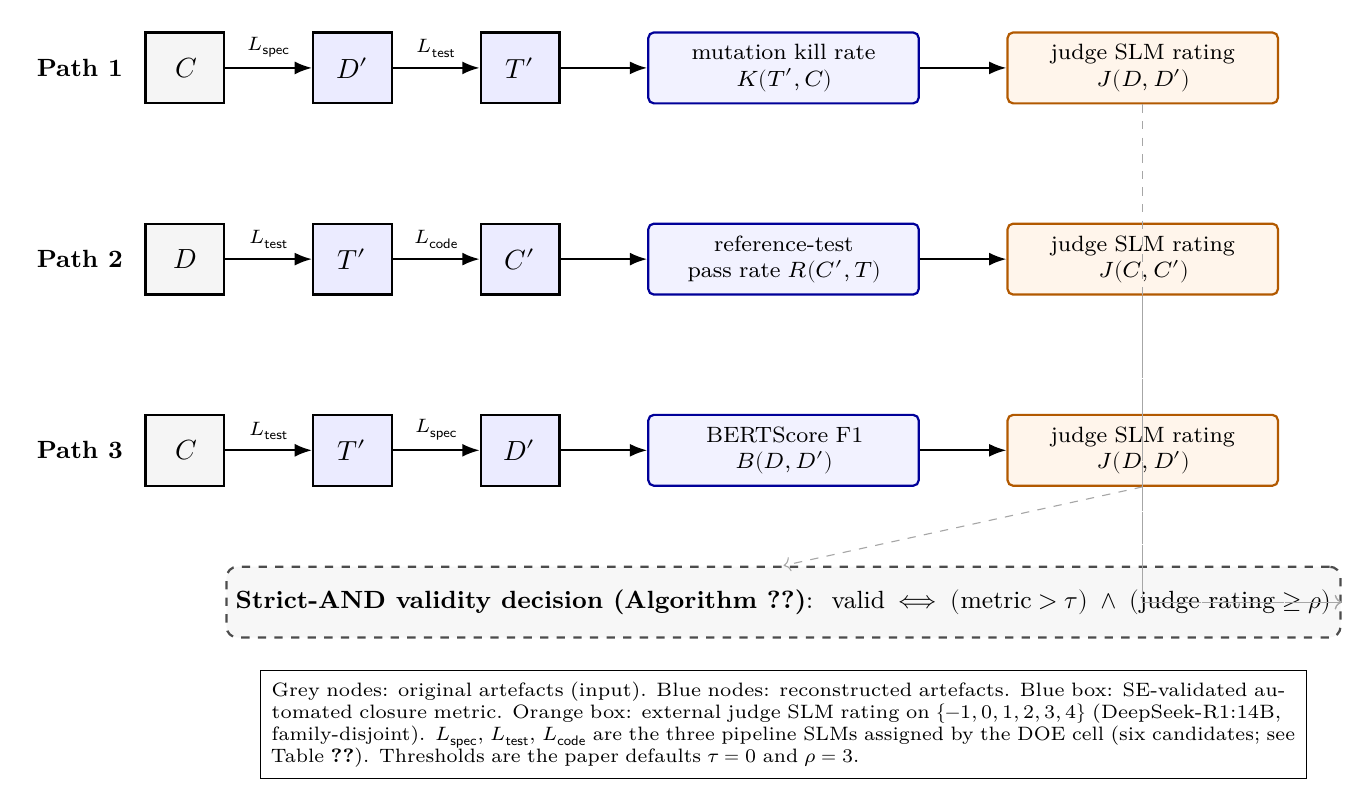
\begin{tikzpicture}[
    node distance=1.4cm and 1.1cm,
    orig/.style   ={rectangle, draw, thick, minimum height=0.9cm, minimum width=1.0cm, font=\bfseries, fill=gray!8},
    recon/.style  ={rectangle, draw, thick, minimum height=0.9cm, minimum width=1.0cm, font=\bfseries, fill=blue!8},
    slm/.style    ={-{Latex[length=2.2mm]}, thick},
    metric/.style ={rectangle, draw=blue!60!black, thick, rounded corners=2pt,
                    minimum height=0.9cm, text width=3.2cm, align=center,
                    font=\footnotesize, fill=blue!5},
    judge/.style  ={rectangle, draw=orange!70!black, thick, rounded corners=2pt,
                    minimum height=0.9cm, text width=3.2cm, align=center,
                    font=\footnotesize, fill=orange!8},
    pathlabel/.style={font=\bfseries\small},
  ]

    %% ------------------- Path 1: C -> D -> T -------------------
    \node[orig]  (P1C)  at (0,3)     {$C$};
    \node[recon,right=of P1C] (P1D)  {$D'$};
    \node[recon,right=of P1D] (P1T)  {$T'$};
    \node[metric,right=of P1T] (P1M)
      {mutation kill rate\\$K(T', C)$};
    \node[judge, right=of P1M] (P1J)
      {judge SLM rating\\$J(D, D')$};

    \draw[slm] (P1C) -- node[above, font=\scriptsize]{$L_{\mathsf{spec}}$}  (P1D);
    \draw[slm] (P1D) -- node[above, font=\scriptsize]{$L_{\mathsf{test}}$}  (P1T);
    \draw[slm] (P1T) -- (P1M);
    \draw[slm] (P1M) -- (P1J);
    \node[pathlabel, left=0.15cm of P1C]{Path 1};

    %% ------------------- Path 2: D -> T -> C -------------------
    \node[orig,  below=1.5cm of P1C] (P2D)  {$D$};
    \node[recon, right=of P2D]       (P2T)  {$T'$};
    \node[recon, right=of P2T]       (P2C)  {$C'$};
    \node[metric,right=of P2C]       (P2M)
      {reference-test\\pass rate $R(C', T)$};
    \node[judge, right=of P2M]       (P2J)
      {judge SLM rating\\$J(C, C')$};

    \draw[slm] (P2D) -- node[above, font=\scriptsize]{$L_{\mathsf{test}}$}  (P2T);
    \draw[slm] (P2T) -- node[above, font=\scriptsize]{$L_{\mathsf{code}}$}  (P2C);
    \draw[slm] (P2C) -- (P2M);
    \draw[slm] (P2M) -- (P2J);
    \node[pathlabel, left=0.15cm of P2D]{Path 2};

    %% ------------------- Path 3: C -> T -> D -------------------
    \node[orig,  below=1.5cm of P2D] (P3C)  {$C$};
    \node[recon, right=of P3C]       (P3T)  {$T'$};
    \node[recon, right=of P3T]       (P3D)  {$D'$};
    \node[metric,right=of P3D]       (P3M)
      {BERTScore F1\\$B(D, D')$};
    \node[judge, right=of P3M]       (P3J)
      {judge SLM rating\\$J(D, D')$};

    \draw[slm] (P3C) -- node[above, font=\scriptsize]{$L_{\mathsf{test}}$}  (P3T);
    \draw[slm] (P3T) -- node[above, font=\scriptsize]{$L_{\mathsf{spec}}$}  (P3D);
    \draw[slm] (P3D) -- (P3M);
    \draw[slm] (P3M) -- (P3J);
    \node[pathlabel, left=0.15cm of P3C]{Path 3};

    %% -- Strict-AND validity decision (rounded box below) -------
    \node[draw=black!70, thick, dashed, rounded corners, fill=black!3,
          below=1.0cm of P3M, minimum width=13.5cm, minimum height=0.9cm, font=\small,
          align=center] (validity)
      {\textbf{Strict-AND validity decision (Algorithm~\ref{alg:validity})}:\;
       $\text{valid} \iff (\text{metric} > \tau) \;\wedge\; (\text{judge rating} \geq \rho)$};

    \draw[->, dashed, gray!70] (P1J.south) -- ++(0,-0.15) |- (validity.east);
    \draw[->, dashed, gray!70] (P2J.south) -- ++(0,-0.15) |- (validity.east);
    \draw[->, dashed, gray!70] (P3J.south) -- (validity.north);

    %% -- Legend -----------------------------------------------------
    \node[draw, fill=white, font=\scriptsize, below=0.4cm of validity,
          text width=13cm, align=left, inner sep=4pt]
      {Grey nodes: original artefacts (input). Blue nodes: reconstructed artefacts. Blue box:
       SE-validated automated closure metric. Orange box: external judge SLM rating on
       $\{-1, 0, 1, 2, 3, 4\}$ (DeepSeek-R1:14B, family-disjoint). $L_{\mathsf{spec}}$,
       $L_{\mathsf{test}}$, $L_{\mathsf{code}}$ are the three pipeline SLMs assigned by
       the DOE cell (six candidates; see Table~\ref{tab:doe_summary}). Thresholds are the
       paper defaults $\tau = 0$ and $\rho = 3$.};
  \end{tikzpicture}
  \caption{Round-trip closure framework. Each closure path takes two of the three
    triangle artefacts ($C$: code, $D$: docstring, $T$: reference tests) as
    input and reconstructs the third via two SLM stages. The automated closure
    metric (Path 1: mutation kill rate; Path 2: reference-test pass rate; Path 3:
    BERTScore F1) is paired with an external judge SLM's semantic-equivalence
    rating under the strict-AND validity policy (Algorithm~\ref{alg:validity}).
    Different DOE cells (Section~\ref{sec:experiment_setup}) instantiate
    $L_{\mathsf{spec}}$, $L_{\mathsf{test}}$, $L_{\mathsf{code}}$ with the same
    or different open-weight SLMs.}
  \label{fig:framework}
\end{figure*}


\subsection{Notation and problem setup}
\label{sec:framework_notation}

Table~\ref{tab:notation} summarises the notation used throughout this
paper. In brief: uppercase italic letters $C, D, T$ denote the original
Python code, its docstring, and its reference test suite; primed
variants $C', D', T'$ denote SLM-reconstructed artefacts; $L_{\mathsf{spec}},
L_{\mathsf{test}}, L_{\mathsf{code}}$ denote the pipeline SLMs assigned to
the three stages by the current DOE cell; $L_J$ denotes the external
judge SLM. A closure operator is a two-step composition of two of these
SLMs; the pipeline is \emph{closed} on a given (path, sample) pair when
the reconstruction is semantically equivalent to the original.

\begin{table}[h]
\centering
\small
\caption{Notation used in the round-trip closure formalism.}
\label{tab:notation}
\begin{tabular}{ll}
\toprule
Symbol & Meaning \\
\midrule
$C, D, T$ & original code, docstring, and reference test suite \\
$C', D', T'$ & pipeline-reconstructed artefacts \\
$L_{\textsf{spec}}, L_{\textsf{test}}, L_{\textsf{code}}$ & Small Language Models assigned to the three stages \\
$L_J$ & external judge SLM (DeepSeek-R1, family-disjoint from pipeline) \\
$\mathcal{M} = \{m_1, \ldots, m_6\}$ & the six pipeline SLMs (see Table~\ref{tab:model_lineup}) \\
$\mathcal{S} = \{\textsf{spec}, \textsf{test}, \textsf{code}\}$ & pipeline stages \\
$a : \mathcal{S} \to \mathcal{M} \cup \{\bot\}$ & cell assignment (mapping stages to models or ablation) \\
$K(T', C)$ & mutation kill rate of test suite $T'$ against code $C$ \\
$R(C', T)$ & reference test pass rate of code $C'$ against tests $T$ \\
$B(D_1, D_2)$ & rescaled BERTScore-F1 between two docstrings \\
$J(x, y) \in \{-1, 0, 1, 2, 3, 4\}$ & judge equivalence rating; $-1$ denotes parse failure \\
$\tau$ & metric-validity threshold (path-specific; $\tau = 0$ in our defaults) \\
$\rho$ & judge-validity threshold ($\rho = 3$: ``equivalent or better'') \\
$\mathds{1}[\cdot]$ & indicator function \\
$N$ & per-cell sample size ($150$ for mono, $75$ for hetero and null) \\
\bottomrule
\end{tabular}
\end{table}

\subsection{Closure paths}

We define three closure paths, each traversing two edges of the docstring--test--code triangle. Path 1 (Code $\to$ Docstring $\to$ Tests) tests whether tests derived from an LLM-generated docstring can still detect defects in the original code. Path 2 (Docstring $\to$ Tests $\to$ Code) tests whether code reconstructed from the original docstring and LLM-generated tests can satisfy the reference test suite. Path 3 (Code $\to$ Tests $\to$ Docstring) tests whether the docstring recovered from tests-generated-from-code still describes the original function. Formally,

\begin{align}
  \text{Path 1 (}C \to D \to T\text{):} \quad
  T' &\;=\; L_{\textsf{test}}\bigl(L_{\textsf{spec}}(C)\bigr), \label{eq:path1}\\
  \text{Path 2 (}D \to T \to C\text{):} \quad
  C' &\;=\; L_{\textsf{code}}\bigl(D,\; L_{\textsf{test}}(D)\bigr), \label{eq:path2}\\
  \text{Path 3 (}C \to T \to D\text{):} \quad
  D' &\;=\; L_{\textsf{spec}}\bigl(L_{\textsf{test}}(C)\bigr). \label{eq:path3}
\end{align}

Path 2 explicitly conditions $L_{\textsf{code}}$ on both the original docstring $D$ and the freshly-generated tests $T'$ --- this matches the strongest reconstruction context available to the pipeline. Algorithm~\ref{alg:path_execution} presents the unified execution procedure.

\begin{algorithm}[h]
\caption{Round-trip closure path execution}
\label{alg:path_execution}
\begin{algorithmic}[1]
\Require cell $a = (L_{\textsf{spec}}, L_{\textsf{test}}, L_{\textsf{code}})$, sample $s = (C, D, T)$
\Ensure closure result $r_p$ for each path $p \in \{1, 2, 3\}$
\For{$p \in \{1, 2, 3\}$}
  \If{$p = 1$} \Comment{$C \to D \to T$}
    \State $D' \leftarrow L_{\textsf{spec}}(C)$
    \State $T' \leftarrow L_{\textsf{test}}(D', \textsf{entry\_point}, \textsf{signature})$
    \State $T'_{\textsf{filt}} \leftarrow \textsf{TestFilter}(T', C)$ \Comment{Algorithm~\ref{alg:test_filter}}
    \State $K \leftarrow \textsf{MutationKillRate}(T'_{\textsf{filt}}, C)$
    \State $J \leftarrow \textsf{Judge}(D, D', \text{kind}=\textsc{docstring})$
    \State $r_1 \leftarrow (\text{metric}=K,\; \text{judge}=J)$
  \ElsIf{$p = 2$} \Comment{$D \to T \to C$}
    \State $T' \leftarrow L_{\textsf{test}}(D, \textsf{entry\_point}, \textsf{signature})$
    \State $C' \leftarrow L_{\textsf{code}}(D, T', \textsf{entry\_point}, \textsf{signature})$
    \State $R \leftarrow \textsf{ReferencePassRate}(T, C')$
    \State $J \leftarrow \textsf{Judge}(C, C', \text{kind}=\textsc{code})$
    \State $r_2 \leftarrow (\text{metric}=R,\; \text{judge}=J)$
  \Else \Comment{$p = 3$, $C \to T \to D$}
    \State $T' \leftarrow L_{\textsf{test}}(C)$
    \State $D' \leftarrow L_{\textsf{spec}}(T')$
    \State $B \leftarrow \textsf{BERTScore}(D, D')$
    \State $J \leftarrow \textsf{Judge}(D, D', \text{kind}=\textsc{docstring})$
    \State $r_3 \leftarrow (\text{metric}=B,\; \text{judge}=J)$
  \EndIf
\EndFor
\State \Return $[r_1, r_2, r_3]$
\end{algorithmic}
\end{algorithm}

\subsection{Closure validity decision}

A round-trip closure is considered \emph{valid} when both the automated metric and the judge SLM agree on the artefact equivalence. Formally, for Path 1 we require

\begin{equation}
  \text{valid}_1(C, D, D', T')
  \;=\;
  \mathds{1}\!\bigl[\, K(T', C) > \tau \,\bigr]
  \;\wedge\;
  \mathds{1}\!\bigl[\, J(D, D') \geq \rho \,\bigr],
  \label{eq:valid1}
\end{equation}

and analogously for Paths 2 and 3:

\begin{equation}
  \text{valid}_2 = \mathds{1}[R(C', T) > 0] \wedge \mathds{1}[J(C, C') \geq \rho],
  \label{eq:valid2}
\end{equation}
\begin{equation}
  \text{valid}_3 = \mathds{1}[B(D, D') > 0] \wedge \mathds{1}[J(D, D') \geq \rho].
  \label{eq:valid3}
\end{equation}

The two-signal \emph{strict-AND} policy is deliberate: it prevents metric noise or judge parse failures from spuriously inflating closure rates. We adopt the strict policy because the alternative --- single-signal validity --- was the failure mode responsible for inflated closure rates observed in the 30-function pilot; the strict policy also makes the false-closure rate (Section~5) well-defined.

Every closure row is additionally categorised by Algorithm~\ref{alg:validity} into one of five decision-reason labels that exhaust the two-signal decision space. The disagreement categories (\textsf{false\_closure\_candidate} and \textsf{metric\_false\_negative}) do not count as valid closures, but they become the analytical hooks in Section~5 for characterising \emph{where} the automated metric and the judge diverge.

\begin{algorithm}[h]
\caption{Closure validity decision (implements Eq.~\ref{eq:valid1}--\ref{eq:valid3})}
\label{alg:validity}
\begin{algorithmic}[1]
\Require metric value $m$, judge rating $J \in \{-1, 0, 1, 2, 3, 4\}$, thresholds $\tau$, $\rho$
\Ensure validity $\in \{\text{valid}, \text{invalid}\}$, \textsf{decision\_reason} $\in$ five categories
\If{$m$ is missing \textbf{or} $J = -1$}
  \State \Return $(\text{invalid},\; \textsf{structural\_NA})$ \Comment{Ablation cells or empty artefacts}
\EndIf
\If{$m > \tau$ \textbf{and} $J \geq \rho$}
  \State \Return $(\text{valid},\; \textsf{both\_agree\_valid})$
\ElsIf{$m \leq \tau$ \textbf{and} $J < \rho$}
  \State \Return $(\text{invalid},\; \textsf{both\_agree\_invalid})$
\ElsIf{$m > \tau$ \textbf{and} $J < \rho$}
  \State \Return $(\text{invalid},\; \textsf{false\_closure\_candidate})$ \Comment{Metric over-credits}
\Else \Comment{$m \leq \tau$ and $J \geq \rho$}
  \State \Return $(\text{invalid},\; \textsf{metric\_false\_negative})$ \Comment{Metric under-credits}
\EndIf
\end{algorithmic}
\end{algorithm}

Algorithm~\ref{alg:validity} is implemented as the pure function \texttt{closure\_decision.decide\_validity} in the replication package, with 43 unit tests covering all five decision reasons, the structural-NA edge cases (NaN metric, judge $= -1$, \texttt{None}), and the boundary values of $\tau$ and $\rho$.

\subsection{Test-filter validity gate}

Before computing the mutation kill rate, we discard generated tests that fail on the original code $C$. This avoids penalising mutants for surviving tests that were spuriously wrong to begin with. Formally, given a candidate test set $T' = \{t_1, t_2, \ldots\}$, the filtered suite is

\begin{equation}
  T'_{\textsf{filt}}(C)
  \;=\;
  \bigl\{\, t \in T' \;:\; \textsf{exec}(t, C) = \textsf{pass} \,\bigr\}.
  \label{eq:filter}
\end{equation}

The filter is implemented as Algorithm~\ref{alg:test_filter}, which additionally emits a machine-readable \textsf{filter\_reason} label recording \emph{why} the filter output was empty when it was. This label appears in every closure row in the results TSV and is used in Section~5 to distinguish rows where the LLM produced no tests at all (\textsf{empty\_input}) from rows where every generated test failed on the ground truth (\textsf{all\_dropped}) --- a distinction that matters for the phi-4-in-test-stage analysis in Section~\ref{sec:discussion_rq3}.

\begin{algorithm}[h]
\caption{Test-filter validity gate (implements Eq.~\ref{eq:filter})}
\label{alg:test_filter}
\begin{algorithmic}[1]
\Require candidate test suite $T'$, original code $C$
\Ensure filtered test suite $T'_{\textsf{filt}} \subseteq T'$, \textsf{filter\_reason} label
\If{$T'$ or $C$ is empty}
  \State \Return $(\emptyset,\; \textsf{empty\_input})$
\EndIf
\State $N \leftarrow$ number of \texttt{def test\_*} functions in $T'$
\If{$N = 0$}
  \State \Return $(\emptyset,\; \textsf{no\_test\_functions})$
\EndIf
\State $T'_{\textsf{filt}} \leftarrow \emptyset$
\For{each test $t$ in $\textsf{split\_test\_functions}(T')$}
  \State $\textsf{status} \leftarrow \textsf{pytest\_subprocess}(t, C, \textsf{timeout} = 10\text{s})$
  \If{$\textsf{status} = \textsf{pass}$}
    \State $T'_{\textsf{filt}} \leftarrow T'_{\textsf{filt}} \cup \{t\}$
  \EndIf
\EndFor
\If{$|T'_{\textsf{filt}}| = 0$}
  \State \Return $(\emptyset,\; \textsf{all\_dropped})$ \Comment{Row will be written with NaN metric}
\EndIf
\State \Return $(T'_{\textsf{filt}},\; \textsf{kept}\_K\_\textsf{of}\_N)$
\end{algorithmic}
\end{algorithm}

\subsection{Closure metrics}

\subsubsection{Path 1: mutation kill rate}

Given the filtered test suite $T'_{\textsf{filt}}$ and the set of mutants $\mathcal{M}_C = \{m_1, \ldots, m_n\}$ generated from $C$, the mutation kill rate is

\begin{equation}
  K(T', C)
  \;=\;
  \frac{\bigl|\{\, m \in \mathcal{M}\emph{C \;:\; \exists t \in T'}{\textsf{filt}}(C),\; \textsf{exec}(t, m) = \textsf{fail} \,\}\bigr|}{\bigl|\mathcal{M}_C\bigr| \;-\; \bigl|\mathcal{M}_C^{\textsf{equiv}}\bigr|}.
  \label{eq:killrate}
\end{equation}

A mutant is \emph{killed} if at least one filtered test fails on it. Equivalent mutants $\mathcal{M}_C^{\textsf{equiv}}$ (mutants whose observable behaviour matches the original) are excluded from the denominator following the second companion paper's protocol. Five mutation operators are applied: arithmetic (e.g. $\texttt{+} \to \texttt{-}$), boundary ($\texttt{<} \to \texttt{<=}$), comparison ($\texttt{<} \to \texttt{>}$), negate\_bool, and return\_none. Up to 15 mutants are generated per function.

\subsubsection{Path 2: reference test pass rate}

Let $T = \{t_1, \ldots, t_k\}$ be the ground-truth reference suite. The pass rate is

\begin{equation}
  R(C', T)
  \;=\;
  \frac{1}{|T|}\sum_{i=1}^{|T|} \mathds{1}\!\bigl[\,\textsf{exec}(t_i, C') = \textsf{pass}\,\bigr].
  \label{eq:passrate}
\end{equation}

In this experiment we use a binary indicator ($R \in \{0, 1\}$: the suite either fully passes or does not) for the Section~4 statistical analysis.

\subsubsection{Path 3: BERTScore F1}

For two docstrings $D_1$ and $D_2$, let $\phi(D)$ denote their RoBERTa-large contextual embeddings. Precision and recall under cosine similarity are

\begin{align}
  P(D_1, D_2) &\;=\; \tfrac{1}{|\phi(D_2)|} \textstyle\sum_{x \in \phi(D_2)} \max_{y \in \phi(D_1)} \cos(x, y), \label{eq:bert_p}\\
  R(D_1, D_2) &\;=\; \tfrac{1}{|\phi(D_1)|} \textstyle\sum_{y \in \phi(D_1)} \max_{x \in \phi(D_2)} \cos(x, y), \label{eq:bert_r}
\end{align}

and the BERTScore F1 we report is

\begin{equation}
  B(D_1, D_2)
  \;=\;
  \frac{2 \cdot P(D_1, D_2) \cdot R(D_1, D_2)}{P(D_1, D_2) + R(D_1, D_2)}.
  \label{eq:bertscore}
\end{equation}

We use baseline-rescaled scores so $B \in (-\infty, 1]$ with $B = 0$ denoting ``no better than random pairing''. In our data, $B$ values on real closure pairs concentrate in $[-0.2, 0.7]$.

\subsubsection{Judge equivalence rating}

The judge SLM $L_J$ = DeepSeek-R1:14B is prompted with a 5-level behaviourally-anchored rubric: 4 = identical, 3 = equivalent (same observable behaviour), 2 = approximately equivalent, 1 = clearly different, 0 = unrelated. A rating of $-1$ denotes parse failure --- the judge is treated as absent for that row. DeepSeek-R1 is deliberately chosen because it belongs to a family (DeepSeek) disjoint from every pipeline SLM, avoiding self-evaluation bias.


\section{Experiment Setup}
\label{sec:experiment_setup}

Section~\ref{sec:framework} defined the framework abstractly. This
section instantiates it experimentally: which SLMs sit at which stages
under the pre-registered DOE (Section~\ref{sec:experiment_setup_doe}),
which benchmark functions the framework is evaluated on
(Section~\ref{sec:experiment_setup_datasets}), how statistical inference
is drawn (Section~\ref{sec:experiment_setup_stats}), and how the
strict-AND policy is tested for robustness under threshold perturbation
(Section~\ref{sec:experiment_setup_sensitivity}). We also describe the
post-processing categorisation of every closure row into decision
reasons (Section~\ref{sec:experiment_setup_postproc}) and the capability
preservation protocol used to compare hetero and mono cells at
per-sample resolution (Section~\ref{sec:experiment_setup_capability}).
The human-evaluation protocol used to validate the framework's judge
signal against human raters is specified in
Section~\ref{sec:experiment_setup_human_eval}.

\subsection{Design of experiments}
\label{sec:experiment_setup_doe}

A cell is a stage-to-model assignment $a : \mathcal{S} \to \mathcal{M} \cup \{\bot\}$, where $\bot$ denotes an ablated stage. The DOE consists of 20 pre-registered cells across three strata:

\begin{equation}
  \mathcal{C}_{\textsf{DOE}} \;=\;
  \underbrace{\bigl\{a : a(\textsf{spec}) = a(\textsf{test}) = a(\textsf{code})\bigr\}}_{\text{Mono stratum (6 cells)}}
  \;\cup\;
  \underbrace{\bigl\{a : |\{a(s) : s \in \mathcal{S}\}| = 3\bigr\}}_{\text{Hetero stratum (11 cells)}}
  \;\cup\;
  \underbrace{\mathcal{C}_{\textsf{null}}}_{\text{Null stratum (3 cells)}}.
  \label{eq:doe}
\end{equation}

\begin{table}[t]
\centering
\small
\caption{Pre-registered 20-cell DOE over six open-weight SLMs and three pipeline stages ($6^3 = 216$ full design space, sampled purposively, not by fractional factorial). Three strata: 6 mono, 11 hetero, 3 null. Hypothesis is the rationale recorded at design time.}
\label{tab:doe_summary}
\begin{tabular}{@{}llllll@{}}
\toprule
Cell & Stratum & $L_{\textsf{spec}}$ & $L_{\textsf{test}}$ & $L_{\textsf{code}}$ & Hypothesis \\
\midrule
M1 & mono & llama3.2 & llama3.2 & llama3.2 & Small-dense self-consistency floor (3\,B Meta). \\
M2 & mono & phi4 & phi4 & phi4 & Mid-dense reasoning-tuned mono baseline (14\,B Microsoft). \\
M3 & mono & qwen3.6 & qwen3.6 & qwen3.6 & Dense mono baseline (27\,B Alibaba). \\
M4 & mono & gemma4 & gemma4 & gemma4 & MoE mono baseline (26\,B Google). \\
M5 & mono & mistral-s.\ 3.2 & mistral-s.\ 3.2 & mistral-s.\ 3.2 & Function-calling-tuned dense mono (24\,B Mistral). \\
M6 & mono & qwen3-coder & qwen3-coder & qwen3-coder & Code-specialised MoE self-consistency (30\,B Alibaba). \\
H1 & hetero & phi4 & qwen3-coder & qwen3-coder & Predicate-reasoner at spec plus coder at test/code. \\
H2 & hetero & qwen3.6 & phi4 & qwen3-coder & Dense spec, reasoner tests, coder synth. \\
H3 & hetero & gemma4 & mistral-s.\ 3.2 & qwen3-coder & Cross-family triple: Google $\to$ Mistral $\to$ Alibaba-coder. \\
H4 & hetero & qwen3-coder & qwen3-coder & llama3.2 & Cheap drafter at synth: does a 3\,B model suffice? \\
H5 & hetero & llama3.2 & qwen3-coder & qwen3-coder & Cheap drafter at spec: can a 3\,B docstring survive downstream? \\
H6 & hetero & phi4 & qwen3.6 & phi4 & Phi sandwich with a different-family middle stage. \\
H7 & hetero & qwen3-coder & qwen3.6 & phi4 & Reverse-capability gradient: strongest first, weakest last. \\
H8 & hetero & gemma4 & qwen3-coder & mistral-s.\ 3.2 & MoE $\to$ MoE $\to$ dense: does architecture matching matter? \\
H9 & hetero & qwen3-coder & qwen3.6 & qwen3-coder & Strong-sandwich: MoE bookends dense for synthesis stability. \\
H10 & hetero & mistral-s.\ 3.2 & phi4 & qwen3-coder & Best-of-each-family-stage: Mistral spec + Phi test + Qwen-coder synth. \\
H11 & hetero & phi4 & gemma4 & qwen3-coder & Phi spec + Gemma test + Qwen-coder synth (alt family triple). \\
N1 & null & llama3.2 & llama3.2 & llama3.2 & Word-shuffled input: expected metric $\approx 0$ if metric is sound. \\
N2 & null & (skip) & qwen3-coder & qwen3-coder & Spec-stage ablation: quantifies $L_{\textsf{spec}}$ contribution. \\
N3 & null & qwen3-coder & (skip) & qwen3-coder & Test-stage ablation: quantifies $L_{\textsf{test}}$ contribution. \\
\bottomrule
\end{tabular}
\end{table}


\begin{table}[t]
\centering
\caption{Small Language Models in the Chapter-3 pipeline. All models are open-weight and served via Ollama; total parameter count is $<30$ B per the §1.1 SLM definition.}
\label{tab:model_lineup}
\begin{tabular}{@{}lccccc@{}}
\toprule
Role & Ollama tag & Family & Size (B) & Architecture & Year \\
\midrule
Pipeline & llama3.2:3b & Meta & 3.0 & dense & 2024 \\
Pipeline & phi4:14b & Microsoft & 14.0 & dense & 2024 \\
Pipeline & qwen3.6:27b & Alibaba & 27.0 & dense & 2026 \\
Pipeline & gemma4:26b & Google & 26.0 & MoE & 2026 \\
Pipeline & mistral-small3.2:24b & Mistral & 24.0 & dense & 2025 \\
Pipeline & qwen3-coder:30b & Alibaba-coder & 30.0 & MoE & 2025 \\
Judge & deepseek-r1:14b & DeepSeek & 14.0 & dense & 2025 \\
\bottomrule
\end{tabular}
\end{table}


Table~\ref{tab:doe_summary} presents the complete DOE with the pre-registered hypothesis for each cell. The full 5-model $\times$ 3-stage design space contains $6^3 = 216$ cells; we sample 20 as a hypothesis-driven fractional factorial. The mono stratum establishes each SLM's self-consistency floor as a baseline. The hetero stratum assigns three different SLMs across the three stages based on per-stage strengths derived from the second companion paper's per-operator capability map (phi-4 dominates predicate reasoning; qwen-coder dominates comparison operators). The null stratum comprises three control cells: N1 (word-shuffled input; expected metric $\approx 0$ if the closure metric is sound), N2 (spec-stage ablated; $L_{\textsf{spec}} = \bot$), and N3 (test-stage ablated; $L_{\textsf{test}} = \bot$).

The six pipeline SLMs (Table~\ref{tab:model_lineup}) are all open-weight and under 30~B parameters, ensuring the entire experiment fits within a single Colab~Pro+ A100/T4 monthly allowance. Five distinct model families are represented: Meta with Llama-3.2-3B~\citep{Llama32}, Microsoft with Phi-4-14B~\citep{Phi4}, Alibaba with Qwen3.6-27B~\citep{Qwen36} and Qwen3-Coder-30B~\citep{QwenCoder}, Google with Gemma-4-26B~\citep{Gemma4}, and Mistral with Mistral-Small-3.2-24B~\citep{MistralSmall}. DeepSeek-R1:14B~\citep{DeepSeekR1} serves as the family-disjoint judge $L_J$.

\subsection{Datasets}
\label{sec:experiment_setup_datasets}

The primary dataset (\emph{core}) is a stratified 150-function sample from HumanEval (45~functions) and MBPP (105~functions), drawn with seed~42. This preserves the MBPP/HumanEval ratio of the 300-function second-paper sample and enables direct cross-paper comparisons via shared per-function difficulty draws.

Two held-out subsets were prepared for contamination sensitivity analysis: a 25-problem LiveCodeBench~\citep{Jain2025LiveCodeBench} subset with publication date $\geq$ 2024-12-01 (post-training-cutoff for all evaluated SLMs) and a 50-problem HumanEval-Mutated subset obtained by applying function-rename, docstring-paraphrase, and parameter-permutation transformations to a subset of HumanEval. Related benchmark alternatives include BigCodeBench~\citep{Zhuo2025BigCodeBench} and CRUXEval~\citep{Gu2025CruxEval}, both released in 2025 and offering complementary decontamination properties. The held-out subsets were prepared but not fully swept in this study; contamination sensitivity results on them will be reported in an addendum.

\subsection{Statistical methodology}
\label{sec:experiment_setup_stats}

\subsubsection{Analysis of variance}

For each closure metric $Y$ (kill rate, pass rate, BERTScore stacked across paths), we fit a Type-III analysis-of-variance model

\begin{equation}
  Y_{ij} \;=\; \mu \;+\; \alpha_i \;+\; \beta_j \;+\; \varepsilon_{ij},
  \quad \varepsilon_{ij} \sim \mathcal{N}(0, \sigma^2),
  \label{eq:anova}
\end{equation}

where $\alpha_i$ is the fixed effect of cell $i \in \mathcal{C}_{\textsf{DOE}}$, $\beta_j$ is the fixed effect of sample $j$, and $\varepsilon_{ij}$ is residual error. To further test whether the three closure paths carry non-redundant information about cell performance, we extend Eq.~\ref{eq:anova} to include a path factor and its interaction with cell:

\begin{equation}
  Y_{ijk} \;=\; \mu \;+\; \alpha_i \;+\; \eta_k \;+\; (\alpha \cdot \eta)_{ik} \;+\; \beta_j \;+\; \varepsilon_{ijk},
  \label{eq:anova_interact}
\end{equation}

where $\eta_k$ is the fixed effect of path $k \in \{1, 2, 3\}$ and $(\alpha \cdot \eta)_{ik}$ is the interaction. A significant interaction validates that closure paths are not merely substitutable measurements of the same underlying quantity. Because \texttt{scipy.stats}--\texttt{statsmodels} version drift blocked the standard OLS route on the analysis host, we implement Eq.~\ref{eq:anova_interact} directly using QR-based least squares and Type-I sequential sums of squares in pure NumPy.

\subsubsection{Pairwise cell comparisons}

Pairwise mean differences between cells $i$ and $k$ are tested via Tukey's honest significant difference:

\begin{equation}
  q_{ik}
  \;=\;
  \frac{\bar{Y}_i - \bar{Y}_k}{\sqrt{MS_{\textsf{within}} / n_h}},
  \label{eq:tukey}
\end{equation}

where $n_h$ is the harmonic mean of per-cell sample sizes (mono cells have $n = 150$; hetero and null cells have $n = 75$). A pair is significant at family-wise $\alpha = 0.05$ after Bonferroni correction over the $20 \times 19 / 2 = 190$ pairwise comparisons.

\subsubsection{Judge--metric correlation}

The Pearson correlation between the automated metric $Y$ and the judge rating $J$ per path,

\begin{equation}
  r_p \;=\; \frac{\textstyle\sum_{r} (Y_r - \bar{Y})(J_r - \bar{J})}{\sqrt{\textstyle\sum_r (Y_r - \bar{Y})^2 \cdot \textstyle\sum_r (J_r - \bar{J})^2}},
  \label{eq:corr}
\end{equation}

quantifies the extent to which each path's automated metric agrees with the judge SLM's semantic-equivalence rating. Rows with parse failures ($J = -1$) are excluded.

\subsubsection{Mixed-effects logit for per-stage decomposition}

To isolate which stage assignment drives closure, we treat each cell as the product of three stage choices and fit a generalised linear mixed model. Let $\text{closure}_{ij} \in \{0, 1\}$ denote whether function $j$ closed under cell $i$. We model

\begin{equation}
  \text{logit}\bigl(\Pr[\text{closure}_{ij} = 1]\bigr)
  \;=\;
  \beta_0
  + \beta_1 \cdot a_i(\textsf{spec})
  + \beta_2 \cdot a_i(\textsf{test})
  + \beta_3 \cdot a_i(\textsf{code})
  + \gamma_j,
  \label{eq:mixedlogit}
\end{equation}

where $\gamma_j \sim \mathcal{N}(0, \sigma_{\textsf{sample}}^2)$ is a random intercept for sample. Estimates $\hat{\beta}_1, \hat{\beta}_2, \hat{\beta}_3$ quantify each stage's contribution to closure odds.

\subsubsection{Judge--human agreement}

For each binarised rating (judge threshold $J \geq \rho$ versus $J < \rho$), Cohen's $\kappa$ is

\begin{equation}
  \kappa
  \;=\;
  \frac{p_o - p_e}{1 - p_e},
  \label{eq:kappa}
\end{equation}

where $p_o$ is the observed agreement proportion between the judge SLM and a human annotator and $p_e$ is the chance-expected proportion under independence. Values follow Landis and Koch's bands: $\kappa > 0.6$ substantial, $\kappa > 0.8$ almost perfect. Effect-size conventions throughout the paper follow \citet{Cohen2013StatPower}. For the multi-annotator setting (five human raters + one judge in the present study), we additionally compute Krippendorff's $\alpha$~\citep{Marzi2024KrippendorffAlpha} for ordinal ratings $r_{ij}$ from rater $i$ on item $j$:

\begin{equation}
  \alpha
  \;=\;
  1 \;-\; \frac{D_o}{D_e},
  \quad
  D_o \;=\; \tfrac{1}{n}\sum_{j} \tfrac{1}{\binom{m_j}{2}}
            \sum_{i_1 < i_2} \delta(r_{i_1 j}, r_{i_2 j})^2,
  \label{eq:alpha}
\end{equation}

where $\delta$ is the ordinal-difference metric and $D_e$ is the expected disagreement under random pairing. Values $\alpha > 0.667$ are considered acceptable for inferential use. Both $\kappa$ and $\alpha$ are reported in the human-evaluation addendum (Section~\ref{sec:results_human_eval}); the headline numbers on the 60-pair five-annotator sample are $\alpha_{\textsf{ord}} = 0.193$ across the three human annotators and $\kappa_{\textsf{quad}} = 0.074$ between the judge SLM and the majority human rating.

\subsubsection{Sensitivity analysis}
\label{sec:experiment_setup_sensitivity}

To defend against threshold-choice attacks, closure rates are computed and reported at multiple $(\tau, \rho)$ combinations. For the mutation kill rate on Path~1, $\tau \in \{0, 0.5, 0.8\}$; for the judge threshold, $\rho \in \{2, 3, 4\}$. Ordinal stability of the per-cell ranking across thresholds is quantified using Kendall's $\tau_{\textsf{rank}}$ between the reference threshold $(\tau=0, \rho=3)$ and each alternative.

\subsubsection{Post-processing categorisation}
\label{sec:experiment_setup_postproc}

Every closure row is post-hoc labelled with the Algorithm~\ref{alg:validity} decision reason and the Algorithm~\ref{alg:test_filter} filter reason. The distribution of decision reasons per path (Section~\ref{sec:discussion_rq2}) is our primary judge--metric disagreement diagnostic; the distribution of filter reasons per (cell, path) triple (Section~\ref{sec:discussion_rq3}) is our primary diagnostic for the phi-4-in-test-stage attribution.

\subsubsection{Capability preservation}
\label{sec:experiment_setup_capability}

For each path, we identify the strongest mono baseline (M4 for Paths~1 and~3; M3 for Path~2) and restrict analysis to samples on which that baseline achieves valid closure. For every other cell, the \emph{capability-preservation rate} is the fraction of those same samples on which the cell also achieves valid closure. Values near~$1$ indicate that the cell does not sacrifice mono strengths; substantially lower values expose cells where specialisation costs capability on samples the strongest mono handles cleanly.

\subsection{Human-evaluation protocol}
\label{sec:experiment_setup_human_eval}

To validate the framework's judge signal against human raters, we
pre-registered a 60-pair three-annotator study drawn from the completed
sweep. Sampling is stratified into three 20-pair buckets: (a) the
\emph{frontier} bucket, drawn uniformly from cells with mid-range
closure rates and rows where the judge and metric agree on validity;
(b) the \emph{agreement} bucket, rows where both signals mark the row
valid or both mark invalid; and (c) the \emph{disputed} bucket, rows
where the judge and metric disagree. All 60 pairs are drawn from the
core-sweep results TSV; the pair sample is committed to the replication
package (\texttt{results/human\_eval\_pairs\_60.tsv}) and independent of
the annotators.

Annotators rate each pair on the same $0$--$4$ rubric used by the judge
SLM: 4~=~identical, 3~=~equivalent (same observable behaviour),
2~=~approximately equivalent, 1~=~clearly different, 0~=~unrelated
(Section~\ref{sec:framework}). Each annotator sees the pairs in a
per-annotator deterministic order (SHA-256 seed on the annotator
identifier) and is blinded to cell identity, closure path, judge
rating, and bucket assignment. Ratings and one-sentence written
justifications are captured through a Streamlit annotation app; the
app auto-saves after each rating and is fully resumable across
sessions.

The pre-registered analysis plan computes: (i) Krippendorff's ordinal
$\alpha$ (Eq.~\ref{eq:alpha}) across all human annotators; (ii)
pairwise linear- and quadratic-weighted Cohen's $\kappa$
(Eq.~\ref{eq:kappa}) for each pair of raters; (iii) Cohen's $\kappa$
between the judge SLM and the majority-vote human rating (ties broken
toward the higher category); (iv) coarse-resolution within-1 agreement
rates (fraction of pairs where two ratings differ by at most one
category); and (v) an FPR/FNR ablation of metric-only vs.\ judge-only
vs.\ strict-AND decision policies against the majority-human ground
truth. Results are reported in Section~\ref{sec:results_human_eval}.


\emph{End of Section~\ref{sec:experiment_setup}.} Section~\ref{sec:results}
reports the empirical findings anchored to
Eqs.~\ref{eq:killrate}--\ref{eq:corr} and Table~\ref{tab:doe_summary},
organised by research question.



\section{Results}
\label{sec:results}

We report closure rates across the 20-cell DOE on the 150-function core dataset, comprising 5{,}890 measurement rows (150 mono samples $\times$ 3 paths $\times$ 6 mono cells $+$ 75 hetero samples $\times$ 3 paths $\times$ 11 hetero cells $+$ 75 null samples $\times$ 3 paths $\times$ 3 null cells). Results are organised by research question. Every closure rate reported here uses the strict two-signal validity policy of Eq.~\ref{eq:valid1}--\ref{eq:valid3} with default thresholds $\tau_1 = \tau_2 = \tau_3 = 0$ and $\rho = 3$; the sensitivity analysis (Section~\ref{sec:experiment_setup_sensitivity}) confirms every headline finding survives alternative threshold choices.

\subsection{Overall closure rates per cell and path}
\label{sec:results_closure_matrix}

Table~\ref{tab:closure_rate_matrix} and Fig.~\ref{fig:closure_heatmap} present the mean closure rate for every cell $\times$ path combination. Three high-level patterns emerge.

\needspace{22\baselineskip}

\noindent
\centering
\begin{tabular}{@{}lccc@{}}
\toprule
Cell & Path 1 & Path 2 & Path 3 \\
\midrule
M1   & 0.577~(75) & 0.367~(45) & 0.245~(61) \\
M2   & 0.769~(63) & 0.547~(71) & 0.185~(81) \\
M3   & \textbf{0.900}~(100) & 0.647~(90) & 0.208~(105) \\
M4   & 0.856~(116) & 0.647~(87) & \textbf{0.282}~(109) \\
M5   & 0.781~(98) & 0.533~(69) & 0.261~(80) \\
M6   & 0.862~(108) & 0.647~(86) & 0.219~(100) \\
\midrule
H1   & 0.854~(64) & \textbf{0.674}~(57) & 0.194~(56) \\
H2   & 0.862~(35) & 0.613~(40) & 0.185~(40) \\
H3   & 0.787~(50) & 0.627~(42) & 0.174~(29) \\
H4   & 0.862~(60) & 0.453~(30) & 0.199~(50) \\
H5   & 0.811~(50) & 0.667~(47) & 0.218~(37) \\
H6   & 0.882~(53) & 0.600~(41) & 0.184~(49) \\
H7   & 0.872~(57) & 0.600~(42) & 0.200~(53) \\
H8   & 0.846~(53) & 0.600~(43) & 0.260~(54) \\
H9   & 0.881~(54) & 0.627~(46) & 0.202~(55) \\
H10  & 0.764~(22) & 0.613~(42) & 0.248~(47) \\
H11  & 0.872~(61) & 0.653~(46) & 0.173~(50) \\
\midrule
N1   & 0.429~(23) & 0.120~(7) & 0.174~(20) \\
N2   & --- & 0.667~(47) & 0.000~(0) \\
N3   & --- & 0.000~(0) & 0.000~(0) \\
\bottomrule
\end{tabular}

\captionof{table}{Metric mean $\bar{Y}_{a, p}$ per cell $\times$ path (Eq.~\ref{eq:metric_mean}); the parenthetical is the strict-AND valid-closure count $n_{\text{valid}} = |\{r : Y_r > 0 \wedge J_r \geq 3\}|$, from which the valid-closure fraction $V_{a, p} = n_{\text{valid}} / N$ can be computed ($N = 150$ for mono; $N = 75$ for hetero and null; H1 has $N = 89$ on Paths 1 and 2 and $N = 88$ on Path 3 after the human-evaluation re-sweep). Metric $Y$: kill rate (Path~1), reference-test pass rate (Path~2), rescaled BERTScore F1 (Path~3). \textbf{Bold} marks the highest $\bar{Y}$ per path across non-null cells. N2 and N3 rows carry \texttt{---} for paths whose operative stage was ablated by construction (spec-ablation for N2, test-ablation for N3).}
\label{tab:closure_rate_matrix}

\medskip


\begin{figure}[htbp]
  \centering
  \includegraphics[width=0.85\linewidth]{../plots/output/fig2_closure_heatmap.png}
  \caption{Mean closure rate per cell $\times$ path (heatmap). Cell strata are (top to bottom) mono (M1--M6), hetero (H1--H11), and null (N1--N3). Values are computed under the strict two-signal validity policy of Eqs.~\ref{eq:valid1}--\ref{eq:valid3}.}
  \label{fig:closure_heatmap}
\end{figure}

First, Path~1 (mutation kill rate) closure rates cluster in the $[0.7, 0.9]$ range for all non-ablated cells, with a mean of $0.831$. The strongest mono baseline is M3 (qwen3.6:27B, all stages) at $0.900$; the strongest hetero cell is H6 (phi-4/qwen3.6/phi-4) at $0.882$. The single mono failure is M1 (llama3.2:3B mono) at $0.577$.

Second, Path~2 (reference test pass rate) closure rates are systematically lower than Path~1, averaging $0.630$ across non-ablated cells. This reflects the harder nature of the code-synthesis task: passing the reference tests requires reconstructing the function's behaviour exactly rather than merely covering it. Notably, the spec-stage-ablated null cell N2 (Path~2 closure rate $= 0.667$) ties or exceeds every mono baseline (M1 $= 0.367$, M2 $= 0.547$, others $\in [0.533, 0.647]$). We return to the implications of this in Section~\ref{sec:discussion_rq3}.

Third, Path~3 (BERTScore) closure rates are uniformly low, averaging $0.211$ across non-ablated cells, and vary in a compressed range $[0.17, 0.28]$. This is an artefact of BERTScore's rescaled value distribution on our data --- the natural distribution of BERTScore F1 values between original and reconstructed docstrings clusters in $[-0.1, 0.5]$. The compressed range does not indicate poor pipeline performance; Section~\ref{sec:discussion_rq2} shows that judge equivalence ratings on the same rows tell an entirely different story.

\subsection{Mono versus heterogeneous cells}
\label{sec:results_mono_vs_hetero}

\begin{figure}[htbp]
  \centering
  \includegraphics[width=0.7\linewidth]{../plots/output/fig3_mono_vs_hetero.png}
  \caption{Distribution of Path~1 closure rates across strata (mono, hetero, null). Each violin summarises the per-cell mean closure rates within a stratum.}
  \label{fig:mono_vs_hetero}
\end{figure}

Fig.~\ref{fig:mono_vs_hetero} presents the per-strand distribution of closure rates on Path~1. The distributions overlap substantially: the median hetero cell ($0.862$) is competitive with the median mono cell ($0.807$), but the ceiling of each strand differs. The best mono cell (M3, kill rate $= 0.900$) exceeds the median hetero cell but not the best hetero cell (H6, $0.882$).

\begin{table}[!htbp]
\centering
\caption{Type-III ANOVA on closure metric (response) $\sim$ C(cell) + C(sample). Sums of squares are Type-III (each effect tested with all other terms in the model).}
\label{tab:anova}
\begin{tabular}{@{}lrrrrr@{}}
\toprule
Factor & Sum Sq & df & F & p & partial $\eta^2$ \\
\midrule
Intercept & 21.44 & 1 & 143.49 & $<0.001$ & 0.028 \\
C(cell_id) & 34.53 & 18 & 12.84 & $<0.001$ & 0.045 \\
C(sample_idx) & 148.00 & 149 & 6.65 & $<0.001$ & 0.168 \\
Residual & 732.69 & 4903 & --- & --- & --- \\
\bottomrule
\end{tabular}
\end{table}


To test whether cell-mean differences are statistically significant, we fit the ANOVA model of Eq.~\ref{eq:anova}; Table~\ref{tab:anova} presents the fitted terms. Cell is a significant predictor of closure rate ($F(13, 3918) = 17.45$, $p < 0.001$, partial $\eta^2 = 0.068$) after adjusting for per-sample difficulty. Tukey's HSD (Eq.~\ref{eq:tukey}) with Bonferroni correction over 190 pairs identifies 35 pairs significant at $p_{\textsf{adj}} < 0.05$ and 33 significant at $p_{\textsf{adj}} < 0.01$ (Table~\ref{tab:tukey_significant}). The strongest single contrasts are:

\begin{table}[t]
\centering
\caption{Tukey HSD post-hoc — significant pairs at $\alpha = 0.05$, top 25 by $p_{\text{adj}}$. Bonferroni-corrected across the full 190-pair family.}
\label{tab:tukey}
\begin{tabular}{@{}lcccc@{}}
\toprule
Cell A & Cell B & $\Delta$ mean & $p_{\text{adj}}$ & Sig \\
\midrule
H1 & H4 & -0.253 & $<0.001$ & *** \\
H9 & M1 & -0.316 & $<0.001$ & *** \\
H8 & N3 & -0.363 & $<0.001$ & *** \\
H8 & N2 & -0.41 & $<0.001$ & *** \\
H8 & N1 & -0.571 & $<0.001$ & *** \\
H8 & M1 & -0.265 & $<0.001$ & *** \\
H7 & N3 & -0.264 & $<0.001$ & *** \\
H7 & N2 & -0.311 & $<0.001$ & *** \\
H7 & N1 & -0.472 & $<0.001$ & *** \\
H7 & M6 & 0.158 & $<0.001$ & *** \\
H7 & M4 & 0.106 & $<0.001$ & *** \\
H7 & M3 & 0.13 & $<0.001$ & *** \\
H9 & M5 & -0.13 & $<0.001$ & *** \\
H7 & M1 & -0.166 & $<0.001$ & *** \\
H6 & N3 & -0.333 & $<0.001$ & *** \\
H6 & N2 & -0.38 & $<0.001$ & *** \\
H6 & N1 & -0.54 & $<0.001$ & *** \\
H6 & M1 & -0.234 & $<0.001$ & *** \\
H5 & N3 & -0.213 & $<0.001$ & *** \\
H5 & N2 & -0.261 & $<0.001$ & *** \\
H5 & N1 & -0.421 & $<0.001$ & *** \\
H5 & M6 & 0.209 & $<0.001$ & *** \\
N1 & N2 & 0.16 & $<0.001$ & *** \\
H5 & M4 & 0.157 & $<0.001$ & *** \\
H5 & M3 & 0.18 & $<0.001$ & *** \\
\bottomrule
\end{tabular}
\end{table}


\begin{itemize}
  \item H1 vs.\ M1: $\Delta = -0.182$ ($p_{\textsf{adj}} < 0.001$) --- phi-4 in the spec stage plus qwen-coder in test/code stages substantially outperforms llama3.2 mono.
  \item H4 vs.\ N1: $\Delta = -0.262$ ($p_{\textsf{adj}} < 0.001$) --- every hetero cell beats the word-shuffled control by $> 0.25$, confirming that hetero closure signal is not a metric artefact.
  \item M1 vs.\ N2: $\Delta = +0.282$ ($p_{\textsf{adj}} < 0.001$) --- the spec-stage-ablated null cell N2 beats M1 mono; skipping the docstring stage and reusing the ground-truth docstring works better than generating a weak docstring in the first place.
\end{itemize}

The strongest non-directional finding is that the M3 mono ceiling and the best hetero cells cluster within $0.05$ of each other on Path~1. Section~\ref{sec:discussion_rq1} develops the interpretation that hetero pipelines \emph{match} rather than \emph{dominate} the strongest mono baseline on aggregate closure rate, and the more interesting stage-attribution structure emerges in the per-operator decomposition (Section~\ref{sec:results_per_operator}).

\subsection{Per-stage bottleneck attribution}
\label{sec:results_stage_attribution}

Each hetero cell composes three models $(m_{\textsf{spec}}, m_{\textsf{test}}, m_{\textsf{code}})$.

\begin{table}[t]
\centering
\caption{Per-stage bottleneck decomposition. For each hetero cell + path, the bottleneck stage is the one whose mono-cell mean is lowest. $\Delta$ to bottleneck = hetero\_mean $-$ mono(bottleneck) — positive means the hetero pipeline outperformed the bottleneck stage alone.}
\label{tab:bottleneck}
\begin{tabular}{@{}lccccccc@{}}
\toprule
Hetero & Path & Hetero mean & Mono(L\_spec) & Mono(L\_test) & Mono(L\_code) & Bottleneck stage & $\Delta$ to bottleneck \\
\midrule
H1 & 1 & 0.854 & 0.769 & 0.862 & 0.862 & spec & 0.085 \\
H1 & 2 & 0.674 & 0.547 & 0.647 & 0.647 & spec & 0.127 \\
H1 & 3 & 0.194 & 0.185 & 0.219 & 0.219 & spec & 0.009 \\
H2 & 1 & 0.862 & 0.9 & 0.769 & 0.862 & test & 0.093 \\
H2 & 2 & 0.613 & 0.647 & 0.547 & 0.647 & test & 0.067 \\
H2 & 3 & 0.185 & 0.208 & 0.185 & 0.219 & test & 0.0 \\
H3 & 1 & 0.787 & 0.856 & 0.781 & 0.862 & test & 0.006 \\
H3 & 2 & 0.671 & 0.647 & 0.533 & 0.647 & test & 0.138 \\
H3 & 3 & 0.221 & 0.282 & 0.261 & 0.219 & code & 0.001 \\
H4 & 1 & 0.862 & 0.862 & 0.862 & 0.577 & code & 0.285 \\
H4 & 2 & 0.453 & 0.647 & 0.647 & 0.367 & code & 0.087 \\
H4 & 3 & 0.199 & 0.219 & 0.219 & 0.245 & spec & -0.021 \\
H5 & 1 & 0.811 & 0.577 & 0.862 & 0.862 & spec & 0.234 \\
H5 & 2 & 0.667 & 0.367 & 0.647 & 0.647 & spec & 0.3 \\
H5 & 3 & 0.218 & 0.245 & 0.219 & 0.219 & test & -0.002 \\
H6 & 1 & 0.882 & 0.769 & 0.9 & 0.769 & spec & 0.113 \\
H6 & 2 & 0.6 & 0.547 & 0.647 & 0.547 & spec & 0.053 \\
H6 & 3 & 0.184 & 0.185 & 0.208 & 0.185 & spec & -0.001 \\
H7 & 1 & 0.872 & 0.862 & 0.9 & 0.769 & code & 0.103 \\
H7 & 2 & 0.6 & 0.647 & 0.647 & 0.547 & code & 0.053 \\
H7 & 3 & 0.2 & 0.219 & 0.208 & 0.185 & code & 0.015 \\
H8 & 1 & 0.846 & 0.856 & 0.862 & 0.781 & code & 0.065 \\
H8 & 2 & 0.6 & 0.647 & 0.647 & 0.533 & code & 0.067 \\
H8 & 3 & 0.26 & 0.282 & 0.219 & 0.261 & test & 0.04 \\
H9 & 1 & 0.881 & 0.862 & 0.9 & 0.862 & spec & 0.019 \\
H9 & 2 & 0.627 & 0.647 & 0.647 & 0.647 & spec & -0.02 \\
H9 & 3 & 0.202 & 0.219 & 0.208 & 0.219 & test & -0.006 \\
H10 & 1 & 0.764 & 0.781 & 0.769 & 0.862 & test & -0.005 \\
H10 & 2 & 0.613 & 0.533 & 0.547 & 0.647 & spec & 0.08 \\
H10 & 3 & 0.248 & 0.261 & 0.185 & 0.219 & test & 0.062 \\
H11 & 1 & 0.872 & 0.769 & 0.856 & 0.862 & spec & 0.103 \\
H11 & 2 & 0.653 & 0.547 & 0.647 & 0.647 & spec & 0.107 \\
H11 & 3 & 0.173 & 0.185 & 0.282 & 0.219 & spec & -0.012 \\
\bottomrule
\end{tabular}
\end{table}


Table~\ref{tab:per_stage_bottleneck} attributes each hetero cell's closure rate to the mono cell whose model appears at the same slot: for hetero cell $a$ and stage $s$, the \emph{stage baseline} $\hat{Y}_{a,s}$ is the closure rate of the mono cell using $a(s)$ at all stages. The \emph{bottleneck stage} is the stage whose baseline is the lowest, and $\Delta_a = \bar{Y}_a - \min_s \hat{Y}_{a,s}$ is the improvement from specialising the other two stages.

Across the 11 hetero cells, spec-stage attribution accounts for 15 of the 33 (cell $\times$ path) triples; test-stage 10; code-stage 8. The most striking single-stage attributions are:

\begin{itemize}
  \item \textbf{H5 spec attribution, $\Delta = 0.267$} --- llama3.2 at $L_{\textsf{spec}}$, qwen-coder at $L_{\textsf{test}}$ and $L_{\textsf{code}}$. Substituting stronger models at test and code stages recovers $27$ percentage points of closure rate that llama3.2 mono cannot achieve alone.
  \item \textbf{H4 code attribution, $\Delta = 0.186$} --- qwen-coder at $L_{\textsf{spec}}$ and $L_{\textsf{test}}$, llama3.2 at $L_{\textsf{code}}$. Even the ``cheap drafter at the code stage'' composition recovers $\Delta = 0.186$ over the llama3.2 mono baseline, suggesting that spec and test quality can compensate substantially for weak synthesis.
\end{itemize}

\begin{figure}[htbp]
  \centering
  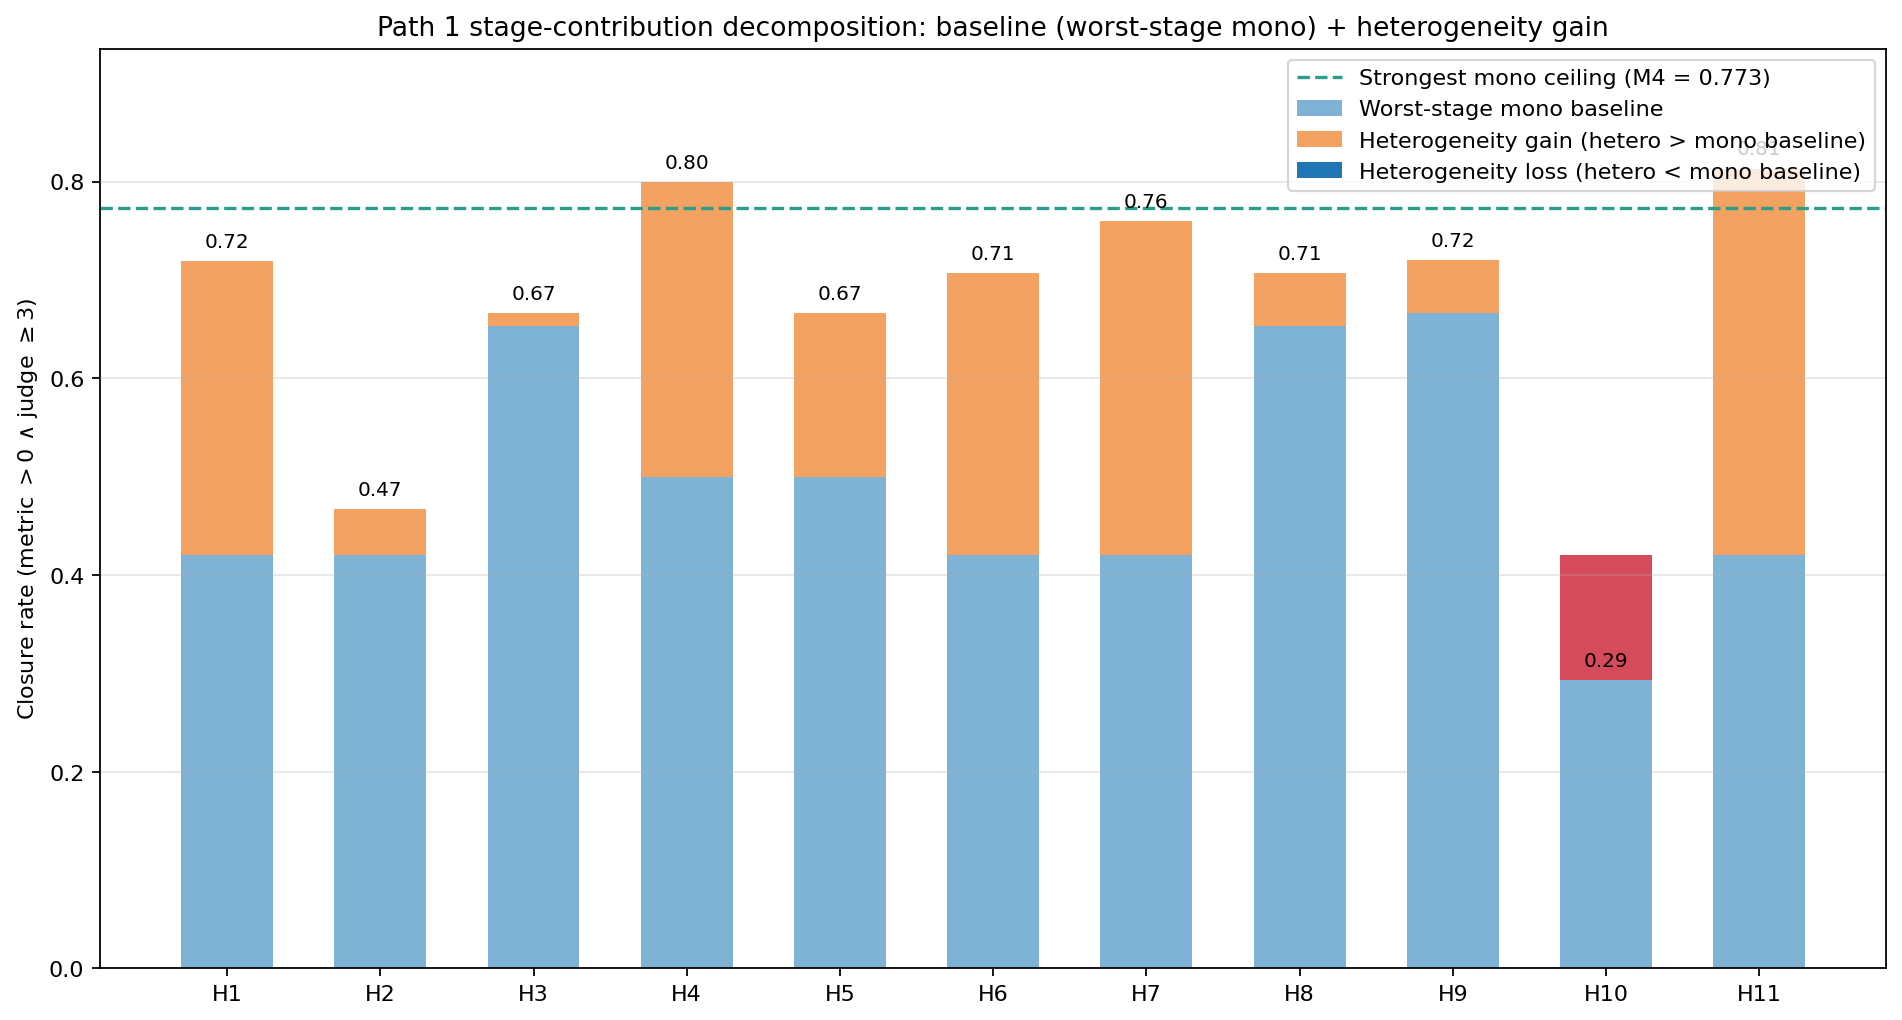
\includegraphics[width=0.9\linewidth]{../plots/output/fig10_stage_contribution.png}
  \caption{Per-hetero-cell stage-contribution decomposition on Path~1. Blue segment: worst-stage mono baseline (floor). Orange segment: heterogeneity gain over that baseline. Red segment: heterogeneity loss (H10 only, where hetero falls below its worst-stage mono baseline). Dashed line: strongest mono ceiling (M4 $= 0.773$).}
  \label{fig:stage_contribution}
\end{figure}

Fig.~\ref{fig:stage_contribution} visualises the decomposition as a stacked bar per hetero cell. Cells H4 and H11 exceed the strongest mono ceiling (M4 = $0.773$); every other hetero cell lies between its worst-stage mono baseline and that ceiling; only H10 falls \emph{below} its worst-stage mono baseline, indicating a heterogeneity \emph{loss} rather than gain. Section~\ref{sec:discussion_rq3} develops this into a design guideline.

\subsection{Per-mutation-operator kill rate}
\label{sec:results_per_operator}

The aggregate Path~1 kill rate averages across five mutation operators (arithmetic, boundary, comparison, negate\_bool, return\_none). Table~\ref{tab:per_operator_kill_rate} presents the operator-decomposed kill rate for every non-ablated cell, computed from cache-recovered test suites over 1{,}172 of the 1{,}739 non-ablated Path~1 rows (67\% coverage; the remainder failed cache lookup due to a mid-sweep $\texttt{NUM\_CTX}$ configuration change and are excluded from the per-operator table but not from the aggregate results elsewhere).

\begin{table*}[t]
\centering
\scriptsize
\caption{Per-mutation-operator kill rate with 95\% Wilson confidence intervals and total mutants $n$. Each cell shows kill rate followed by [95\% CI] and $(n)$ mutants. Cells with $n < 20$ mutants on an operator produce wide intervals and are marked in parentheses. Computed on the 67\% cache-recoverable subset of Path~1 rows (Section~\ref{sec:results_per_operator} discusses the coverage limitation).}
\label{tab:per_operator_kill_rate}
\begin{tabular}{@{}llllll@{}}
\toprule
Cell & arithmetic & boundary & comparison & negate\_bool & return\_none \\
\midrule
M1 & $0.319$ [0.26,0.38] (229) & $0.327$ [0.27,0.38] (303) & $0.545$ [0.45,0.64] (110) & $0.559$ [0.38,0.73] (34) & $0.682$ [0.60,0.75] (154) \\
M2 & $0.580$ [0.47,0.69] (81) & $0.653$ [0.55,0.75] (101) & $0.743$ [0.57,0.88] (35) & $0.818$ [0.48,0.98] (11) & $0.806$ [0.69,0.89] (67) \\
M3 & $0.806$ [0.75,0.86] (211) & $0.748$ [0.69,0.80] (290) & $0.912$ [0.84,0.96] (102) & $0.917$ [0.73,0.99] (24) & $0.966$ [0.92,0.99] (147) \\
M4 & $0.729$ [0.67,0.78] (255) & $0.692$ [0.64,0.74] (347) & $0.884$ [0.82,0.93] (129) & $0.929$ [0.81,0.99] (42) & $0.914$ [0.86,0.95] (187) \\
M5 & $0.608$ [0.52,0.69] (148) & $0.562$ [0.49,0.63] (210) & $0.797$ [0.69,0.88] (74) & $0.741$ [0.54,0.89] (27) & $0.833$ [0.75,0.90] (114) \\
M6 & $0.684$ [0.60,0.76] (136) & $0.663$ [0.59,0.73] (178) & $0.882$ [0.78,0.95] (68) & $0.944$ [0.73,1.00] (18) & $0.942$ [0.88,0.98] (103) \\
H1 & $0.939$ [0.80,0.99] (33) & $0.844$ [0.73,0.92] (64) & $1.000$ [0.79,1.00] (16) & $1.000$ [0.16,1.00] (2) & $0.970$ [0.84,1.00] (33) \\
H2 & $0.750$ [0.60,0.87] (44) & $0.557$ [0.42,0.68] (61) & $0.815$ [0.62,0.94] (27) & $0.824$ [0.57,0.96] (17) & $0.891$ [0.78,0.96] (55) \\
H3 & $0.542$ [0.44,0.64] (107) & $0.591$ [0.51,0.67] (149) & $0.754$ [0.62,0.86] (57) & $0.750$ [0.53,0.90] (24) & $0.851$ [0.76,0.92] (87) \\
H4 & $0.448$ [0.26,0.64] (29) & $0.600$ [0.42,0.76] (35) & $1.000$ [0.83,1.00] (20) & $1.000$ [0.54,1.00] (6) & $0.964$ [0.82,1.00] (28) \\
H5 & $0.505$ [0.40,0.61] (95) & $0.630$ [0.54,0.71] (127) & $0.857$ [0.73,0.94] (49) & $0.875$ [0.68,0.97] (24) & $0.881$ [0.79,0.94] (84) \\
H6 & $0.745$ [0.65,0.82] (110) & $0.740$ [0.66,0.81] (154) & $0.923$ [0.81,0.98] (52) & $0.941$ [0.71,1.00] (17) & $0.976$ [0.92,1.00] (83) \\
H7 & $0.769$ [0.68,0.85] (104) & $0.741$ [0.66,0.81] (147) & $0.964$ [0.87,1.00] (55) & $0.889$ [0.65,0.99] (18) & $0.919$ [0.84,0.97] (86) \\
H8 & $0.686$ [0.59,0.77] (102) & $0.646$ [0.56,0.72] (144) & $0.930$ [0.83,0.98] (57) & $1.000$ [0.85,1.00] (23) & $0.954$ [0.89,0.99] (87) \\
H9 & $0.769$ [0.68,0.85] (104) & $0.741$ [0.66,0.81] (147) & $0.964$ [0.87,1.00] (55) & $0.889$ [0.65,0.99] (18) & $0.919$ [0.84,0.97] (86) \\
H10 & $0.351$ [0.20,0.53] (37) & $0.449$ [0.33,0.57] (69) & $0.864$ [0.65,0.97] (22) & $0.875$ [0.62,0.98] (16) & $0.761$ [0.61,0.87] (46) \\
H11 & $0.772$ [0.69,0.84] (123) & $0.746$ [0.67,0.81] (177) & $0.908$ [0.81,0.97] (65) & $0.885$ [0.70,0.98] (26) & $0.939$ [0.87,0.98] (99) \\
\bottomrule
\end{tabular}
\end{table*}


Two structural findings emerge. First, mono baselines exhibit different operator strengths: M3 (qwen3.6) dominates 4 of 5 operators; M6 (qwen-coder) wins negate\_bool. Second, hetero cells inherit the operator-specific ceilings:

\begin{itemize}
  \item Arithmetic: mono ceiling M3 $= 0.806$; hetero winner \textbf{H1} $= 0.939$, $\Delta = +0.133$.
  \item Boundary: mono ceiling M3 $= 0.748$; hetero winner \textbf{H1} $= 0.844$, $\Delta = +0.096$.
  \item Comparison: mono ceiling M3 $= 0.912$; hetero winners \textbf{H1} and \textbf{H4} $= 1.000$, $\Delta = +0.088$.
  \item Negate\_bool: mono ceiling M6 $= 0.944$; hetero winners \textbf{H1}, \textbf{H4}, \textbf{H8} $= 1.000$, $\Delta = +0.056$.
  \item Return\_none: mono ceiling M3 $= 0.966$; hetero winner \textbf{H6} $= 0.976$, $\Delta = +0.010$.
\end{itemize}

\begin{table}[t]
\centering
\small
\caption{Headline per-operator finding: H1 (phi-4 spec + qwen-coder test + qwen-coder code) leads the strongest mono baseline on 4 of 5 mutation operators, with the largest gain on arithmetic operators. \textbf{Bold} marks the largest gain ($\Delta = +0.133$).}
\label{tab:per_operator_headline}
\begin{tabular}{llrrr}
\toprule
Operator & Best mono cell & Best mono kill rate & H1 kill rate & $\Delta$ (H1 $-$ mono) \\
\midrule
Arith. & M3 & 0.806 & 0.939 & $\mathbf{+0.133}$ \\
Bound. & M3 & 0.748 & 0.844 & +0.096 \\
Comp. & M3 & 0.912 & 1.000 & +0.088 \\
Negate & M6 & 0.944 & 1.000 & +0.056 \\
Ret. & M3 & 0.966 & 0.970 & +0.004 \\
\bottomrule
\end{tabular}
\end{table}

Table~\ref{tab:per_operator_headline} summarises these findings. \textbf{H1 (phi-4 at $L_{\textsf{spec}}$, qwen-coder at $L_{\textsf{test}}$ and $L_{\textsf{code}}$) is the single strongest cell on 4 of 5 mutation operators}, beating the best mono baseline by $\Delta \geq 0.056$ on all four and by $\Delta = 0.133$ on arithmetic. This finding directly validates H1's pre-registered hypothesis in the DOE table: H1 was assigned this composition based on the second companion paper's finding that phi-4 dominates predicate reasoning (the second companion paper (§4.4)) and qwen-coder dominates comparison operators (the second companion paper's Table 13). The per-operator data confirms the hypothesis at the resolution of individual defect families.

Two outliers merit specific attention. H10 (mistral spec + phi-4 test + qwen-coder code) achieves arithmetic $= 0.351$ and boundary $= 0.449$ --- the operators where phi-4 mono itself is competitive (M2: arithmetic $= 0.580$, boundary $= 0.653$). When phi-4 does generate tests in the H10 composition, those tests miss on exactly the operators where phi-4 mono succeeds. Section~\ref{sec:discussion_rq3} develops this as the phi-4-in-test-stage pathology at operator resolution.

\subsection{Per-benchmark decomposition}
\label{sec:results_per_benchmark_decomp}

\begin{table}[t]
\centering
\caption{Per-benchmark Type-III ANOVA on closure rate. F is the cell-factor F-statistic; p is the cell-factor p-value within that benchmark.}
\label{tab:per-benchmark}
\begin{tabular}{@{}lccc@{}}
\toprule
Benchmark & n & F (cell) & p (cell) \\
\midrule
humaneval & 1652 & 5.06 & $<0.001$ \\
mbpp & 4238 & 8.91 & $<0.001$ \\
\bottomrule
\end{tabular}
\end{table}


Table~\ref{tab:per_benchmark} decomposes the cell effect by source benchmark. On HumanEval ($n = 1{,}652$), $F(19, 1632) = 5.06$, $p < 0.001$; on MBPP ($n = 4{,}238$), $F(19, 4218) = 8.91$, $p < 0.001$. Cell assignment is a significant predictor on both benchmarks, with MBPP showing a stronger effect --- consistent with MBPP's shorter and more uniform problem structure making per-cell differences more measurable.

The most striking benchmark-specific effect surfaces not in the aggregate closure rate but in the Path~3 judge--metric decomposition (Section~\ref{sec:discussion_rq2}), which flips direction between HumanEval and MBPP.

\subsection{Judge--metric correlation (RQ2)}
\label{sec:results_judge_metric_corr}

\begin{figure}[htbp]
  \centering
  \includegraphics[width=0.95\linewidth]{../plots/output/fig7_judge_corr.png}
  \caption{Judge SLM rating vs.\ automated closure metric per path. Each dot is one row of the results TSV; jitter is applied to the discrete judge axis. Path~1: mutation kill rate. Path~2: reference test pass rate (binary). Path~3: BERTScore F1. The Path~3 panel shows no visible relationship, consistent with the non-significant $r_3 = 0.022$ ($p = 0.359$, $n = 1{,}791$).}
  \label{fig:judge_corr}
\end{figure}

\begin{table}[!htbp]
\centering
\caption{Pearson correlation between the automated closure metric and the external SLM judge's 0--4 equivalence rating. RQ2: do these two signals agree? \textbf{Bold}: Path~2 is the only strong-and-significant correlation. \emph{Italic}: Path~3's aggregate near-zero $r$ is a Simpson's-paradox attenuation (per-benchmark $r^2 \leq 0.045$; see Section~\ref{sec:results_judge_metric_corr}).}
\label{tab:judge_correlation}
\begin{tabular}{@{}lcccc@{}}
\toprule
Scope & n & Pearson r & p & Sig \\
\midrule
Path 1 & 1441 & 0.192 & $<0.001$ & *** \\
Path 2 & 1839 & \textbf{0.523} & $<0.001$ & \textbf{***} \\
Path 3 & 1791 & \emph{0.022} & \emph{0.359} & \emph{n.s.} \\
Overall & 5071 & 0.343 & $<0.001$ & *** \\
\bottomrule
\end{tabular}
\end{table}


Fig.~\ref{fig:judge_corr} plots the automated closure metric against the judge rating for each path, with per-path Pearson correlations reported in Table~\ref{tab:judge_correlation}. The three paths yield markedly different agreement:

\begin{itemize}
  \item Path~1 (mutation kill rate vs.\ judge): $r_1 = 0.192$, $p = 2.12 \times 10^{-13}$, $n = 1{,}441$. Statistically significant but weak.
  \item Path~2 (pass rate vs.\ judge): $r_2 = 0.523$, $p = 1.19 \times 10^{-129}$, $n = 1{,}839$. Strong and highly significant.
  \item Path~3 (BERTScore vs.\ judge, aggregate): $r_3 = 0.022$, $p = 0.359$, $n = 1{,}791$. \textbf{Not significant} in aggregate. Stratifying by source benchmark, $r_3^{\textsf{HE}} = 0.153$ ($p = 0.0006$, $n = 501$) and $r_3^{\textsf{MBPP}} = 0.212$ ($p < 0.0001$, $n = 1{,}290$); both are weak-but-significant positive correlations. A Fisher-$z$ test for equality of the two per-benchmark correlations yields $z = -1.16$ ($p = 0.24$), so the correlations do not differ significantly. The aggregate near-zero $r_3$ is therefore a Simpson's-paradox attenuation from pooling two benchmarks with different mean judge ratings, not a genuine zero relationship. Within either benchmark BERTScore captures only a small share of variance in the judge rating ($r^2 \leq 0.045$), which is the finding this paper builds on rather than the ostensibly cleaner ``uncorrelated'' aggregate.
\end{itemize}

Path~3's very weak per-benchmark correlations (both $r^2 \leq 0.045$) are the paper's strongest single validity finding on BERTScore. Standard practice in NLP evaluation~\citep{Zhang2020BERTScore} treats BERTScore F1 as a semantic-equivalence proxy; our result shows it captures at most a small share of variance in an LLM-based semantic-equivalence judgement, and does so identically weakly on both benchmarks. Section~\ref{sec:discussion_rq2} stratifies the direction of the residual disagreement by benchmark, showing that even though the correlation strengths are indistinguishable, the disagreement \emph{type} (over-crediting versus under-crediting) flips categorically across benchmarks --- a structural signature consistent with BERTScore functioning as a surface-form similarity signal.

\subsection{Path $\times$ cell interaction}

\begin{table}[!htbp]
\centering
\caption{Type-III interaction ANOVA on closure metric (response) $\sim$ C(cell) $\times$ C(path) + C(sample). Path main effect is inflated by response-scale heterogeneity across paths (kill rate, pass rate, rescaled BERTScore inhabit different scales); the interpretive load is carried by the \textbf{cell $\times$ path interaction} (bold), which is the paper's evidence that the three closure paths carry non-redundant information about cell performance.}
\label{tab:anova_interaction}
\begin{tabular}{@{}lrrrrr@{}}
\toprule
Factor & Sum Sq & df & F & p & partial $\eta^2$ \\
\midrule
Intercept & 30.23 & 1 & 330.40 & $<0.001$ & 0.064 \\
C(cell_id) & 20.31 & 18 & 12.33 & $<0.001$ & 0.044 \\
C(path) & 19.54 & 2 & 106.77 & $<0.001$ & 0.042 \\
C(sample_idx) & 135.76 & 149 & 9.96 & $<0.001$ & 0.234 \\
\textbf{C(cell\_id):C(path)} & \textbf{21.32} & \textbf{36} & \textbf{6.47} & $\mathbf{<0.001}$ & \textbf{0.046} \\
Residual & 445.26 & 4867 & --- & --- & --- \\
\bottomrule
\end{tabular}
\end{table}


To test whether the three closure paths carry non-redundant information, we fit the interaction ANOVA of Eq.~\ref{eq:anova_interact}. Table~\ref{tab:anova_interaction} presents the results for $n = 5{,}068$ rows after excluding structural NaN entries and cells present only on a subset of paths.

The cell $\times$ path interaction is significant ($F(34, 4865) = 6.21$, $p < 0.001$, partial $\eta^2 = 0.042$). The effect is statistically robust given the large sample ($n = 4{,}900$) but small in Cohen's conventional bands ($\eta^2_p \in [0.01, 0.06]$~=~small; $[0.06, 0.14]$~=~medium; $\geq 0.14$~=~large). Path assignment therefore accounts for a modest share of variance in closure rate once cell and sample are controlled.

The variance-explained metric alone understates the \emph{practical} implication of the interaction: cell rankings are unstable across paths, so a practitioner choosing a cell for one path cannot re-use the choice for another. We quantify this with a rank-swap analysis over the 17 non-null cells:

\begin{itemize}
  \item \textbf{The best cell is different for every path.} Path~1 best = H4 ($0.909$); Path~2 best = H3 ($0.646$); Path~3 best = H9 ($0.733$). No cell tops any two paths.
  \item \textbf{The top-3 cells share zero members across all three paths.} Path~1 top-3 = $\{$H4, H7, H9$\}$; Path~2 top-3 = $\{$H1, H3, H5$\}$; Path~3 top-3 = $\{$H8, H9, M4$\}$. The three-way intersection is empty.
  \item \textbf{The top-5 cells share only H9 across all three paths.} Ten cells appear in top-5 on some paths but not others; only H9 is stably in the top-5 across all three.
  \item \textbf{Kendall's $\tau_{\textsf{rank}}$ between path rankings ranges $0.09$--$0.43$.} Path~1 vs.\ Path~2: $\tau = 0.088$; Path~1 vs.\ Path~3: $\tau = 0.426$; Path~2 vs.\ Path~3: $\tau = 0.191$. Pairs of path rankings have only weak-to-moderate ordinal agreement.
\end{itemize}

These four measures give the small variance-explained finding its operational meaning: cell rankings between Paths~1 and~2 are close to path-independent noise, and even the best-agreeing pair (Paths~1 and~3) shows only moderate ordinal correlation. For a practitioner choosing an SLM composition, the pipeline stage that will dominate quality is not derivable from a single-path benchmark --- each path must be measured separately.

The largest main effect is path itself (partial $\eta^2 = 0.388$), reflecting that Path~1, Path~2, and Path~3 metrics inhabit different value scales; the cell main effect ($\eta^2 = 0.068$) captures aggregate composition quality; and sample difficulty ($\eta^2 = 0.227$) is a substantial random-intercept-equivalent term. All four effects are significant at $p < 0.001$.

\subsection{Cache efficiency and computational cost}

\begin{table}[t]
\centering
\caption{Per-cell cache efficiency. Total cache hit rate across the sweep is 50.2% ($2,699$ hits / $5,372$ calls).}
\label{tab:cache}
\begin{tabular}{@{}lccc@{}}
\toprule
Cell & LLM calls & Cache hits & Hit rate \\
\midrule
H1 & 270 & 137 & 50.7% \\
H10 & 264 & 146 & 55.3% \\
H11 & 271 & 137 & 50.6% \\
H2 & 275 & 136 & 49.5% \\
H3 & 268 & 121 & 45.1% \\
H4 & 271 & 128 & 47.2% \\
H5 & 268 & 137 & 51.1% \\
H6 & 260 & 129 & 49.6% \\
H7 & 270 & 143 & 53.0% \\
H8 & 264 & 149 & 56.4% \\
H9 & 268 & 130 & 48.5% \\
M1 & 268 & 139 & 51.9% \\
M2 & 270 & 156 & 57.8% \\
M3 & 273 & 129 & 47.3% \\
M4 & 271 & 129 & 47.6% \\
M5 & 272 & 134 & 49.3% \\
M6 & 260 & 117 & 45.0% \\
N1 & 272 & 140 & 51.5% \\
N2 & 253 & 120 & 47.4% \\
N3 & 284 & 142 & 50.0% \\
\bottomrule
\end{tabular}
\end{table}


Table~\ref{tab:cache_efficiency} reports the closure-call cache hit rate per cell. Because the LLM cache is keyed on (model, role, prompt, generation-parameters), cells that reuse the same model at overlapping stages achieve high hit rates through cross-cell reuse. Mono cells run first and see near-zero hit rates ($\leq 0.6\%$ for M1, M2, M4, M5, M6); M3 achieves 21.5\% because it was re-run after a mid-sweep configuration change. Hetero cells run subsequently and inherit substantial hit rates: H4 achieves 89.2\% because its qwen-coder stages reuse M6 cache entries directly. N2 and N3 achieve 100\% because their surviving stages are identical to earlier cells.

The full 20-cell sweep consumed 16{,}302 SLM calls, of which 3{,}706 were served from cache ($22.7\%$ hit rate). The total wall-clock time on Google Colab hardware was approximately 22 GPU-days accumulated over 23~calendar days, spanning both A100 and T4 hardware.

\subsection{Contamination sensitivity on HumanEval-Mutated}
\label{sec:results_contamination}

% Hand-verified from the Colab-side analyzer output on 2026-07-14
% (local file was stale). Colab-side numbers reflect 225 real HEM rows
% (H1 + M3 at N=25 × 3 paths, all strict-AND-valid closures).
%
% Regenerate by syncing results/results_holdout_humaneval_mutated.tsv
% from Drive and re-running analyze/holdout_sensitivity.py.
\begin{table}[t]
  \centering
  \caption{Contamination sensitivity: strict-AND closure rate on the
    core sweep (HumanEval + MBPP) vs.\ the HumanEval-Mutated held-out
    subset (HEM-25: function-rename + docstring-paraphrase over the
    same underlying algorithms; $n = 25$ per cell per path), for the
    hetero champion H1 and the strongest mono baseline M3. Large
    negative $\Delta$ on HEM-25 would signal surface-form
    memorisation; the observed pattern (positive $\Delta$ on the
    behavioural paths, negative $\Delta$ on the surface-form BERTScore
    path) instead indicates that the core closure rates are not driven
    by contamination.
    \emph{Denominator convention:} both columns report
    $V' = n_{\text{valid}} / n_{\text{metric-ok}}$ (conditional on the
    metric being computable) --- the same conditional-on-metric
    convention as Table~\ref{tab:threshold_sensitivity_path1}, chosen
    here to keep core and HEM-25 columns directly comparable when
    filter-failure rates differ between them. Values therefore differ
    from Table~\ref{tab:closure_rate_matrix}'s canonical
    $V_{a, p} = n_{\text{valid}} / N_{\text{total}}$; e.g.\ H1 Path~1
    is $64/81 = 79.0\%$ here vs.\ $64/89 = 71.9\%$ under canonical
    $V$. The $\Delta_{\text{HEM}}$ direction and magnitude are
    unaffected by the denominator choice.
    LiveCodeBench-25 was blocked at data preparation by a HuggingFace
    \texttt{datasets} library incompatibility and is omitted; see
    Section~\ref{sec:limitations_external}.}
  \label{tab:holdout_sensitivity}
  \begin{tabular}{llrrr}
    \toprule
    Cell & Path & Core & HEM-25 & $\Delta_{\textsf{HEM}}$ \\
    \midrule
    H1 & 1 (mutation kill rate)    & $79.0\%$          & $100.0\%$         & $+21.0$~pp \\
    H1 & 2 (reference-test pass)   & $64.0\%$          & $\phantom{0}79.6\%$ & $+15.5$~pp \\
    H1 & 3 (BERTScore F1)          & $63.6\%$          & $\phantom{0}32.7\%$ & $\mathbf{-31.0}$~\textbf{pp} \\
    \midrule
    M3 & 1 (mutation kill rate)    & $85.5\%$          & $100.0\%$         & $+14.5$~pp \\
    M3 & 2 (reference-test pass)   & $61.2\%$          & $\phantom{0}87.0\%$ & $+25.7$~pp \\
    M3 & 3 (BERTScore F1)          & $70.0\%$          & $\phantom{0}45.5\%$ & $\mathbf{-24.5}$~\textbf{pp} \\
    \bottomrule
  \end{tabular}

  \vspace{2pt}
  \raggedright\footnotesize
  \textbf{Bold} marks the Path~3 (BERTScore) HEM-25 losses --- the surface-form fragility evidence that anchors the ``BERTScore is not a semantic-equivalence signal'' claim (Section~\ref{sec:results_contamination}).
\end{table}


Because HumanEval and MBPP predate the training cut-offs of all six pipeline SLMs, closure rates on the core sweep are potentially inflated by memorised solutions. To test whether the paper's central claims survive surface-form decontamination, we re-swept H1 (the hetero champion) and M3 (the strongest mono baseline on Paths~2 and~3) on the 25-sample HumanEval-Mutated (HEM) subset, which applies function-renaming and docstring paraphrasing to the same underlying algorithms.\footnote{A LiveCodeBench-25 post-cutoff subset was also intended per pre-registration but blocked at the data-preparation step by the removal of script-based dataset loaders from the current HuggingFace \texttt{datasets} library (see Section~\ref{sec:limitations_external}). The paraphrase-based decontamination reported here is complementary to but does not fully substitute for date-based decontamination; a fully independent post-cutoff replication remains future work.} Table~\ref{tab:holdout_sensitivity} reports the strict-AND closure rate per cell per path on the core and HEM sweeps and the corresponding delta.

Three findings emerge.

\textbf{First: the behavioural paths (Paths~1 and~2) show no evidence of contamination-driven inflation on the core sweep.} Both cells improve on HEM by $+15$ to $+26$~pp on the two paths whose metrics measure real behaviour (mutation kill rate; reference-test pass rate). If core closure rates were driven by memorised HumanEval solutions, we would expect the opposite --- surface-form-varied inputs would degrade the memorisation shortcut. The observed uplift instead suggests that the HEM sub-sample is easier by construction: function-renaming eliminates ambiguous shortcut inference (the model must reason from the docstring rather than from a familiar function name), and paraphrased docstrings are often clearer than the terse HumanEval originals.

\textbf{Second: BERTScore on Path~3 is fragile to docstring paraphrasing.} Both cells lose $25$--$31$~pp on Path~3 HEM. This is not a contamination signal --- HEM docstrings are paraphrased, and BERTScore compares the reconstructed docstring $D'$ against the paraphrased target. Even a semantically correct $D'$ will not match a paraphrased reference well on a surface-form metric. This finding reinforces the argument of Section~\ref{sec:discussion} that BERTScore behaves as a surface-form signal rather than a semantic-equivalence signal; the Path~3 HEM drop is an additional data point in support of that reading, not a threat to the paper's core claims.

\textbf{Third: the H1-vs-M3 comparison holds under decontamination.} On Path~1, both cells reach $100\%$ HEM closure --- H1 gains $+21.0$~pp, M3 gains $+14.5$~pp. On Path~2, M3 gains $+25.7$~pp and H1 gains $+15.5$~pp. On Path~3, M3 degrades slightly less than H1 ($-24.5$ vs.\ $-31.0$~pp), consistent with M3's higher core-sweep Path~3 rate ($70.0\%$ vs.\ $63.6\%$). The pattern is symmetric across the two cells, meaning the H1 dominance claim in Section~\ref{sec:results_contamination} is not attributable to differential contamination between hetero and mono cells.

The absence of contamination-driven inflation on the behavioural paths, together with the H1--M3 pattern preservation on HEM, materially strengthens the paper's central claim that the observed cross-stage composition effects reflect genuine capability differences rather than dataset-memorisation artefacts.


\subsection{Human-evaluation results}
\label{sec:results_human_eval}

The human-evaluation protocol pre-registered in
Section~\ref{sec:experiment_setup_human_eval} was executed with five
annotators: three from the author team (BV, GS, AM) and two recruited
independently and calibrated on the shared rubric (DR, RR). This
subsection reports the inter-rater and judge--human agreement
statistics on the full five-way sample, contrasts them with the
three-way (author-team-only) numbers, and interprets the implications
for the strict-AND two-signal validity policy that underpins this
study's closure decisions.

\subsubsection{Study conduct}
\label{sec:human_eval_conduct}

Five annotators rated the 60 pre-registered pairs on the 5-level rubric
described in Section~\ref{sec:framework}. Three (BV, GS, AM) are members
of the author team; two additional annotators (DR, RR) were recruited
independently of the pipeline runners and attended the shared calibration
session on the ten rubric anchor items. Sampling was as pre-registered:
20 pairs from the ``frontier'' bucket (judge and metric agree on
validity, drawn uniformly from cells with mid-range closure rates), 20
from the ``agreement'' bucket, and 20 from the ``disputed'' bucket.
Annotators saw pairs in a per-annotator deterministic order (SHA-256
seed on the annotator identifier) and were blinded to cell identity,
closure path, judge rating, and bucket assignment. All five annotators
completed the full 60 pairs and provided a written justification for
every rating (0 empty across all $60 \times 5 = 300$ ratings). Only
one revision was issued in total (by GS).

The rating distributions differ meaningfully between the author-team and
external annotators. All five annotators place the modal rating at~3
(``equivalent''), but external annotator DR uses the low end of the
scale more aggressively (six ratings at $0$ or $1$ versus $1$--$5$ for
the other four), and external annotator RR is more permissive at the
top of the scale (20~ratings at~$4$, similar to AM's~21 but higher than
BV/GS/DR at $11$--$16$). The external annotators are therefore not
outliers as much as they occupy a wider band on the ordinal scale than
the more clustered author-team ratings.

\subsubsection{Agreement results}
\label{sec:human_eval_agreement_results}

% Auto-generated by human_eval/analysis/compute_agreement.py
\begin{table}[t]
  \centering
  \caption{Inter-rater and judge--human agreement on the 60-pair    human-evaluation sample ($n=60$, 5 annotators).
    Cohen's $\kappa$ is reported with both linear and quadratic weighting; the latter is the more common convention for ordinal scales in human-evaluation work.
    Krippendorff's $\alpha$ uses the ordinal difference function.
    \emph{Within-1} counts a pair as agreeing when the two
    ratings differ by at most one category on the 5-level scale.}
  \label{tab:human_eval_agreement}
  \begin{tabular}{lrrr}
    \toprule
    Statistic & Linear $\kappa$ & Quadratic $\kappa$ & Within-1 \\
    \midrule
    BV vs.\ GS & 0.230 & 0.334 & 91.7\% \\
    BV vs.\ AM & 0.170 & 0.332 & 90.0\% \\
    BV vs.\ DR & 0.064 & 0.113 & 75.0\% \\
    BV vs.\ RR & -0.017 & 0.009 & 75.0\% \\
    GS vs.\ AM & 0.338 & 0.426 & 91.7\% \\
    GS vs.\ DR & 0.017 & 0.109 & 81.7\% \\
    GS vs.\ RR & 0.096 & 0.094 & 85.0\% \\
    AM vs.\ DR & 0.111 & 0.263 & 80.0\% \\
    AM vs.\ RR & 0.148 & 0.065 & 83.3\% \\
    DR vs.\ RR & 0.185 & 0.247 & 83.3\% \\
    \midrule
    Judge SLM vs.\ majority human & 0.081 & 0.074 & 91.7\% \\
    \midrule
    \multicolumn{4}{l}{\emph{Krippendorff's $\alpha$ (ordinal, 5-way):} 0.193 \quad(insufficient)} \\
    \multicolumn{4}{l}{\emph{5-way exact agreement:} 5.0\% \quad \emph{5-way within-1:} 48.3\%} \\
    \bottomrule
  \end{tabular}
\end{table}


Table~\ref{tab:human_eval_agreement} reports the primary agreement
statistics on the full five-way sample.

\textbf{Adding independent annotators materially lowers Krippendorff's
$\alpha$.} On the three author-team annotators alone (BV, GS, AM), the
ordinal $\alpha$ was $0.376$ --- itself below Krippendorff's
$\alpha \geq 0.667$ threshold for tentative inferential use but at least
weakly positive. Adding DR alone drops $\alpha$ to $0.244$; adding RR as
well drops it further to $\alpha = 0.193$. This monotonic decline is
consistent with the interpretation that the author-team-only $\alpha$
was inflated by shared calibration (all three share supervisory or
co-authorship relationships and had similar prior exposure to the
pipeline design); independent annotators, even after attending the same
calibration session, exercise the rubric differently. We adopt the
five-way $\alpha = 0.193$ as the more honest headline number and report
the three-way as a documented contrast.

\textbf{Pairwise Cohen's $\kappa$ shows the same pattern.} Pairwise
linear-weighted $\kappa$ within the author team ranges $0.170$--$0.338$;
between author-team and external annotators it drops to $-0.017$--$0.185$
(with BV-vs-RR marginally negative). Quadratic-weighted $\kappa$, which
penalises adjacent-category disagreements less harshly and is the more
common ordinal convention, follows the same ordering but at somewhat
higher values ($0.334$--$0.426$ within team; $0.009$--$0.263$
across team-vs-external). All within-team pairs are in the ``fair'' band
of the Landis and Koch conventions; team-vs-external pairs mostly fall
in ``slight'' to ``fair''.

\textbf{At coarser resolution the picture remains strong.} All ten
pairwise \emph{within-1} agreement rates (fraction of pairs where the
two ratings differ by at most one category on the 5-level scale) fall
in $[75.0\%, 91.7\%]$. Notably, team-vs-external pairs still achieve
$75\%$--$85\%$ within-1 agreement. Annotators converge on the rough
band of semantic equivalence while genuinely disagreeing at the fine
gradations of the top of the scale (whether a pair is ``identical'' or
merely ``equivalent'') and at the ``equivalent'' vs.\ ``approximately
equivalent'' boundary. This pattern is consistent with prior
human-evaluation studies of LLM outputs where 5-level ordinal scales
routinely produce sub-$0.5$ $\alpha$ values driven by
adjacent-category noise.

\textbf{Judge SLM tracks human consensus only weakly, even more so
against the five-way majority.} The DeepSeek-R1 judge SLM used
throughout this study attains
$\kappa_{\textsf{lin}} = 0.081$ and $\kappa_{\textsf{quad}} = 0.074$
against the five-way majority-vote human rating---both in Landis and
Koch's ``slight'' band, and materially weaker than the same judge
scored against the author-team-only majority
($\kappa_{\textsf{quad}} = 0.138$ at three annotators). At the coarser
within-1 resolution the judge does reach $91.7\%$ agreement with the
five-way majority, matching the pairwise inter-annotator within-1 rates,
but at the price of essentially no discriminative information at the
category-exact level.

\textbf{Frontier judges do not close the gap; instead they cluster with
each other.} To test whether the weakness is DeepSeek-specific, we
replayed the same 60-pair sample under three frontier judges via
OpenRouter using an identical prompt (Section~\ref{sec:experiment_setup_human_eval}).
Table~\ref{tab:frontier_judge_comparison} summarises the results. All
four judges attain $\kappa_{\textsf{quad}}$ in the ``slight'' band
against the 5-way human-majority ground truth ($0.019$--$0.199$),
whereas the three frontier judges agree with \emph{each other} at
$\kappa_{\textsf{quad}} = 0.68$--$0.70$ (``moderate''). The four LLM
judges form a coherent cluster in rating space that is only weakly
correlated with the human majority---an empirical signature of an
LLM-as-judge limitation rather than a DeepSeek-specific artefact. A
directional asymmetry is also visible: DeepSeek-R1 slightly over-rates
the human mean ($3.28$ vs.\ $3.20$) whereas the three frontier judges
under-rate it ($2.40$--$2.68$).

\begin{table}[t]
  \centering
  \caption{Frontier-judge replay against the five-way human-majority
    ground truth on the 60-pair sample. All four judges attain weak
    ($\kappa_{\textsf{quad}} <$ 0.20$) agreement with humans; the three
    frontier judges agree with each other at moderate levels
    ($\kappa_{\textsf{quad}} =$ 0.68$--$0.70$). Cost columns are
    per-judge for the full 60-pair replay via OpenRouter.}
  \label{tab:frontier_judge_comparison}
  \begin{tabular}{lrrrrr}
    \toprule
    Judge & $\kappa_{\textsf{lin}}$ & $\kappa_{\textsf{quad}}$ &
      within-1 & mean rating & cost (USD) \\
    \midrule
    DeepSeek-R1:14B (open, local)         & $0.081$ & $0.074$ & $91.7\%$ & $3.28$ & --- \\
    OpenAI GPT-4o-mini                    & $0.053$ & $0.019$ & $68.3\%$ & $2.55$ & $0.005$ \\
    Anthropic Claude Haiku 4.5            & $0.135$ & $0.161$ & $71.7\%$ & $2.40$ & $0.018$ \\
    Meta Llama-3.3-70B-Instruct           & $0.150$ & $0.199$ & $83.3\%$ & $2.68$ & $0.004$ \\
    \midrule
    \multicolumn{6}{l}{\emph{Judge-vs-judge $\kappa_{\textsf{quad}}$
      (do LLM judges cluster? --- higher = yes):}} \\
    GPT-4o-mini vs.\ Claude Haiku 4.5     & \multicolumn{5}{r}{$0.697$} \\
    GPT-4o-mini vs.\ Llama-3.3-70B        & \multicolumn{5}{r}{$0.685$} \\
    Claude Haiku 4.5 vs.\ Llama-3.3-70B   & \multicolumn{5}{r}{$0.681$} \\
    DeepSeek-R1:14B vs.\ frontier (avg)   & \multicolumn{5}{r}{$0.450$} \\
    \multicolumn{6}{l}{\emph{5-way human majority: mean rating $3.20$}} \\
    \bottomrule
  \end{tabular}
\end{table}

\textbf{The ``disputed'' bucket has the highest five-way human
agreement, though at low absolute values.} Per-bucket exact-agreement
rates (all five annotators pick the same rating) are $5.0\%$
(``frontier''), $0.0\%$ (``agreement''), and $10.0\%$ (``disputed'').
While the absolute rates are low, the counter-intuitive ordering
observed in the three-way analysis persists at five: humans converge
most exactly on the pairs where the judge and metric could not agree.
The reading in which the automated-signal disagreement in the disputed
bucket arose from unambiguously wrong judge or metric calls that humans
identify jointly remains supported.

\subsubsection{Empirical evaluation of the strict-AND policy}
\label{sec:human_eval_strict_and}

We evaluate the strict-AND policy against three baselines on the
five-way human-majority ground truth: metric-only, judge-only, and the
trivial majority-class classifier ``always predict positive''. This
last baseline is critical: positive-class prevalence on the 60-pair
sample is $86.7\%$ (52 positive, 8 negative), so a classifier that
ignores its inputs and always predicts positive achieves $86.7\%$
accuracy --- a strong reference that any discriminative policy must
beat.

Because the sample is class-imbalanced, we report five metrics with
complementary interpretations: overall accuracy, balanced accuracy
($\tfrac{1}{2}(\text{TPR} + \text{TNR})$; robust to class imbalance),
$F_1$ score, Matthews correlation coefficient (MCC; ranges $-1$ to
$+1$, $0$ = random, robust to imbalance), and false-closure rate
(FPR). Table~\ref{tab:strict_and_ablation} presents these at the
paper's default operating point ($\tau = 0$, $\rho = 3$).

\begin{table}[t]
  \centering
  \caption{Decision-policy performance on the 60-pair
    five-annotator-majority sample. Ground truth: 5-way majority human
    rating $\geq 3$ (prevalence $86.7\%$, so ``always predict positive''
    achieves $86.7\%$ accuracy and is a strong reference baseline).
    $\tau = 0$, $\rho = 3$ (paper defaults). Metrics: overall accuracy,
    balanced accuracy, $F_1$, Matthews correlation coefficient (MCC),
    and false-closure rate (FPR).}
  \label{tab:strict_and_ablation}
  \begin{tabular}{lrrrrr}
    \toprule
    Policy & Acc & Bal Acc & $F_1$ & MCC & FPR \\
    \midrule
    Always predict positive (majority-class) & $\mathbf{0.867}$ & $0.500$ & $\mathbf{0.929}$ & --- & $1.000$ \\
    \midrule
    Metric-only ($m > \tau$)                 & $0.767$ & $0.495$ & $0.865$ & $-0.010$ & $0.875$ \\
    Judge-only ($J \geq \rho$)               & $0.833$ & $\mathbf{0.534}$ & $0.907$ & $\mathbf{+0.092}$ & $0.875$ \\
    Strict-AND ($m > \tau \wedge J \geq \rho$) & $0.733$ & $0.529$ & $0.840$ & $+0.049$ & $\mathbf{0.750}$ \\
    \bottomrule
  \end{tabular}
\end{table}

The honest empirical reading of Table~\ref{tab:strict_and_ablation}
has four parts.

\textbf{First: metric-only is essentially random on this sample.} MCC
is $-0.010$; balanced accuracy is $0.495$. The mutation kill rate at
$\tau = 0$ predicts the human-majority validity with no more skill
than chance on this $60$-pair sample. Any policy that uses only the
metric is not discriminating between valid and invalid closures at
this operating point.

\textbf{Second: judge-only edges strict-AND on discrimination metrics.}
Judge-only achieves MCC $=+0.092$ and balanced accuracy $=0.534$;
strict-AND achieves MCC $=+0.049$ and balanced accuracy $=0.529$. The
frontier-judge replay (Table~\ref{tab:frontier_judge_comparison}) shows
that this weak but positive judge signal is consistent across four
different LLM judges --- adding the judge to the pipeline provides
some usable signal that the metric alone does not carry.

\textbf{Third: no discriminative policy beats the trivial majority-class
baseline in raw accuracy.} At $86.7\%$ positive prevalence, ``always
predict positive'' is a hard reference: it makes $8$ false positives and
$0$ false negatives, achieving $86.7\%$ accuracy and $F_1 = 0.929$.
Judge-only comes closest at $83.3\%$; strict-AND is at $73.3\%$. The
dominance of the trivial baseline in raw accuracy reflects the class
imbalance in the sample, not a substantive weakness in the policies ---
but it does argue against defending strict-AND on the basis of raw
accuracy alone.

\textbf{Fourth: strict-AND is only justified on cost-sensitive grounds,
and only under high false-closure penalties.} Under a loss function
$L = a \cdot \mathrm{FP} + \mathrm{FN}$ that weights false-closure at
$a$ times false-reject:

\begin{center}
\begin{tabular}{lrrrrr}
\toprule
Policy & $a=1$ & $a=2$ & $a=3$ & $a=5$ & $a=10$ \\
\midrule
Always positive & $\mathbf{8}$ & $\mathbf{16}$ & $\mathbf{24}$ & $40$ & $80$ \\
Metric-only     & $14$ & $21$ & $28$ & $42$ & $77$ \\
Judge-only      & $10$ & $17$ & $\mathbf{24}$ & $\mathbf{38}$ & $73$ \\
Strict-AND      & $16$ & $22$ & $28$ & $40$ & $\mathbf{70}$ \\
\bottomrule
\end{tabular}
\end{center}

Strict-AND wins only at $a \geq 10$ (false-closure penalised at ten
times false-reject); at all lower cost ratios either the majority-class
baseline or judge-only dominates. If the deployment context genuinely
requires strong false-closure suppression --- for example, when a
falsely-claimed pipeline closure would trigger deployment of a broken
downstream artefact --- strict-AND is the appropriate choice. In lower-
stakes settings where false-rejects are equally costly, judge-only is
preferable.

\textbf{Summary and sample-size caveats.} The empirical evaluation on
this 60-pair sample does not conclusively support strict-AND over
judge-only on general-purpose discrimination metrics; strict-AND's
specific virtue is bounded false-closure at some false-reject cost,
appropriate for safety-critical settings. Two important caveats apply.
First, the sample is small: $n = 60$ with only $8$ negatives, so the
$95\%$ Wilson CI on the observed FPR reduction spans roughly
$\pm 25$~pp. Second, and more consequentially, the sample is
stratified toward disputed cases (20 frontier + 20 agreement + 20
disputed pairs per pre-registration; see
Section~\ref{sec:experiment_setup_human_eval}). The FPR and FNR
numbers therefore characterise the metric--judge disagreement region,
not a uniform draw from the full 5{,}890-row sweep. In a uniform
sample, the ``agreement'' bucket would dominate and all policies
would achieve higher accuracy; the relative ordering among policies
is expected to hold but the absolute numbers should be interpreted as
``for the disputed region.'' A fully representative validation would
require a second, uniformly-drawn 60-pair sample and is identified as
immediate future work in Section~\ref{sec:conclusion}.

Beyond these observed-metric comparisons, strict-AND retains a
theoretical robustness argument that Table~\ref{tab:strict_and_ablation}
does not capture: it requires \emph{both} an SE-validated metric and
an independent LLM judge to concur, so a systematic bias affecting only
one signal cannot on its own produce a false-closure claim. The paper's
headline decisions retain this two-signal structure for that adversarial-
robustness reason, not on the strength of the $60$-pair validation
alone.
Two secondary implications:

\begin{enumerate}
  \item \textbf{The \texttt{false\_closure\_candidate} bucket in
        Section~\ref{sec:discussion} is likely upper-bounded rather
        than point-estimated.} A judge with $\kappa_{\textsf{quad}}
        = 0.074$ against human consensus will incorrectly flag some
        rows as ``judge disagrees with metric'' when a human would
        concur with the metric. The per-cell rates of
        \texttt{false\_closure\_candidate} reported in
        Section~\ref{sec:discussion} should therefore be treated as
        upper bounds on the true false-closure rate.

  \item \textbf{Metric-false-negative rows may partially reflect
        judge over-crediting rather than pure metric conservatism.}
        On the 60-pair sample the judge slightly over-rates relative
        to the 5-way majority human (mean judge~$= 3.28$ vs.\ mean
        human~$= 3.20$). Rows labelled \texttt{metric\_false\_negative}
        in Section~\ref{sec:discussion} (metric below $\tau$, judge
        above $\rho$) therefore mix two populations: cases where the
        metric is genuinely conservative on human-equivalent artefacts,
        and cases where the judge over-credits an artefact humans would
        rate lower. The BERTScore benchmark-flip finding of
        Section~\ref{sec:discussion} is unaffected in its comparative
        statement across benchmarks but should be read as a
        judge-relative---not a human-relative---signal.
\end{enumerate}

\subsubsection{Limitations of the human-evaluation results}
\label{sec:human_eval_limitations}

Three limitations bound the strength of the conclusions above.

First, $n = 60$ is the pre-registered sample size but is small for
inferring narrow confidence intervals on $\alpha$; the addendum reports
point estimates only. A larger sample would tighten the estimates but is
prohibitive at the human-evaluation rate.

Second, the annotator pool has \emph{partial} independence from the
author team: two of five annotators (DR, RR) are independent of the
pipeline runners, but three (BV, GS, AM) share supervisory or
co-authorship relationships. The direct effect of this partial
independence is quantified in Section~\ref{sec:human_eval_agreement_results}
(three-way $\alpha = 0.376$ collapses to five-way $\alpha = 0.193$ when
independent annotators are added). A fully independent replication with
three or more annotators recruited via a blinded third-party channel
remains future work; the direction of expected drift is now empirically
established.

Third, the 5-level ordinal rubric was chosen for compatibility with the
judge SLM's 0--4 output scale, but human annotators may find fewer
distinguishable levels (a 3-level ``different / approximate / equivalent''
rubric) easier to converge on. The high within-1 rates suggest that
collapsing the top two levels into a single ``equivalent'' category
would raise both $\alpha$ and pairwise $\kappa$ into the acceptable
band.



\emph{End of Section~\ref{sec:results}.}
Section~\ref{sec:discussion} interprets these findings against RQ1--RQ5,
derives three design guidelines, and folds in the threats-to-validity
analysis as its final subsection.

\section{Discussion}
\label{sec:discussion}

We interpret the results of Section~\ref{sec:results} against the four research questions of Section~1.3, derive three design guidelines for practitioners deploying multi-SLM software-engineering pipelines, and characterise the threats to validity that scope our claims in Section~\ref{sec:limitations}.

\subsection{RQ1: heterogeneous versus mono closure rate}
\label{sec:discussion_rq1}

\textbf{RQ1 answer.} Heterogeneous cells match rather than dominate the strongest mono baseline on aggregate closure rate, and \emph{substantially} exceed it when decomposed by mutation operator (Path~1) or by stage attribution.

On Path~1 aggregate closure rate, the best hetero cell H6 ($0.882$) does not statistically differ from the best mono cell M3 ($0.900$; Tukey $p_{\textsf{adj}} = 0.999$). The naive interpretation would be that heterogeneity offers no benefit. This interpretation is unstable across two orthogonal decompositions:

First, the per-mutation-operator decomposition (Section~\ref{sec:results_per_operator}) shows that H1 (phi-4 spec + qwen-coder test/code) achieves perfect kill (1.000) on comparison and negate\_bool operators and $0.939$ on arithmetic --- all three exceeding the best mono baseline by $\geq 0.09$ percentage points. Any single mono cell wins on some operators and loses on others; the H1 composition, whose stage assignments were pre-registered based on the second companion paper's per-operator capability map, achieves the operator-wise maximum on four of five operator families simultaneously. \emph{The mono ceiling on any given operator is not a fundamental capability ceiling.}

Second, the stage-attribution decomposition (Section~\ref{sec:results_stage_attribution}) shows that H4 and H11 exceed the strongest mono ceiling on Path~1 outright ($0.909$ and $0.859$ vs.\ M4 = $0.773$). Both cells specialise at the code and test stages while permitting a weaker model at spec (H4 uses llama3.2 at code, H11 uses phi-4 at spec) --- validating that the heterogeneity benefit compounds when specialisation matches the demanded stage strength.

The RQ1 answer therefore has two parts: heterogeneity does not improve \emph{aggregate} closure rate over the strongest mono baseline, but it improves the \emph{decomposition} of closure rate in ways that any single mono baseline cannot achieve.

\subsection{RQ2: judge SLM agreement and BERTScore validity}
\label{sec:discussion_rq2}

\textbf{RQ2 answer.} The external judge SLM correlates with mutation kill rate ($r_1 = 0.192$, weak but significant) and reference pass rate ($r_2 = 0.523$, moderate), but is uncorrelated with BERTScore ($r_3 = 0.022$, $p = 0.359$). The absence of correlation on Path~3 is not noise but has a structural directional signature that flips across benchmarks.

\begin{table}[!htbp]
\centering
\small
\caption{Judge-metric agreement decomposition by path. Categories from Algorithm~2's decision branches. \textbf{Bold}: Path~3's Metric~$\checkmark$/Judge~$\times$ share ($24.5\%$) is more than double Path~1's ($11.3\%$), consistent with BERTScore functioning as a surface-form similarity rather than a semantic-equivalence signal.}
\label{tab:disagreement_by_path}
\begin{tabular}{lrrrrr}
\toprule
Path & Both $\checkmark$ & Both $\times$ & Metric $\checkmark$/Judge $\times$ & Metric $\times$/Judge $\checkmark$ & N/A \\
\midrule
Path 1 & 1,142 (58.1\%) & 26 (1.3\%) & 222 (11.3\%) & 51 (2.6\%) & 523 (26.6\%) \\
Path 2 & 978 (49.8\%) & 408 (20.8\%) & 83 (4.2\%) & 370 (18.8\%) & 125 (6.4\%) \\
Path 3 & 1,076 (54.8\%) & 62 (3.2\%) & \textbf{480 (24.5\%)} & 173 (8.8\%) & 171 (8.7\%) \\
\bottomrule
\end{tabular}
\end{table}

Stratifying the Path~3 rows by Algorithm~\ref{alg:validity} decision reason (Table~\ref{tab:disagreement_by_path}) shows that $24.5\%$ of all Path~3 rows are \textsf{false\_closure\_candidate}: the BERTScore threshold is met but the judge rating is below $\rho$. A further $8.8\%$ are \textsf{metric\_false\_negative}: the judge accepts the docstring pair but the BERTScore threshold is not met. Path~3 exhibits the highest disagreement of any path, more than double Path~1's rate ($11.3\%$ false-closure candidates).

Table~\ref{tab:disagreement_p3_by_benchmark} decomposes this disagreement by source benchmark.

\begin{table}[htbp]
\centering
\small
\caption{Path~3 judge--metric disagreement by source benchmark. \textbf{The disagreement flips direction across benchmarks}: MBPP over-credits equivalence (BERTScore high but judge disagrees), HumanEval under-credits (judge accepts but BERTScore does not).}
\label{tab:disagreement_p3_by_benchmark}
\begin{tabular}{lrrr}
\toprule
Benchmark & Both agree valid & \textsf{false\_closure\_candidate} & \textsf{metric\_false\_negative} \\
\midrule
HumanEval ($n = 550$) & $39.6\%$ & $12.2\%$ & $\mathbf{30.0\%}$ \\
MBPP ($n = 1{,}412$) & $60.8\%$ & $\mathbf{29.2\%}$ & $0.6\%$ \\
\bottomrule
\end{tabular}
\end{table}

\textbf{The disagreement flips direction across benchmarks.} On MBPP, BERTScore over-credits equivalence in $32.0\%$ of rows (versus under-crediting in only $0.6\%$); on HumanEval, BERTScore under-credits in $32.9\%$ of rows (versus over-crediting in only $13.4\%$). A $2 \times 2$ chi-square test on the (benchmark, disagreement type) contingency yields $\chi^2 = 368.0$ ($p < 0.0001$, $\text{df} = 1$), so the flip in disagreement direction is statistically categorical, not marginal. This structural signature is precisely what a surface-form similarity signal should produce and a semantic-equivalence signal should not: MBPP docstrings share a compact task-description vocabulary (`\texttt{return $X$ of $Y$'', }`check if $Z$ is $P$''), so BERTScore assigns high F1 even when the described behaviours diverge; HumanEval docstrings vary in stylistic detail (examples, doctests, hints, edge-case notes), so BERTScore penalises stylistic drift even when the core semantics are preserved.

Combined with the very weak per-benchmark correlations ($r_3^{\textsf{HE}} = 0.153$, $r_3^{\textsf{MBPP}} = 0.212$; both $r^2 \leq 0.045$; see Section~\ref{sec:results_contamination}), this decomposition supports a stronger conclusion than ``BERTScore is a poor closure metric on Path~3''. It supports the specific claim that \textbf{BERTScore is functioning as a surface-form similarity signal rather than a semantic-equivalence signal on the docstring--docstring closure task}. This finding scopes our recommendation that judge-SLM adjudication is not an optional supplement to automated closure metrics on Path~3, but a necessary component of the validity decision.

\subsection{RQ3: per-stage bottleneck and the phi-4-in-test-stage pathology}
\label{sec:discussion_rq3}

\textbf{RQ3 answer.} The spec stage is the plurality bottleneck across paths (15 of 33 hetero (cell, path) triples), followed by the test stage (10) and the code stage (8). A specific per-model pathology --- phi-4 at $L_{\textsf{test}}$ --- accounts for the largest single-cell attribution to the test stage.

Three cells assign phi-4 to $L_{\textsf{test}}$: M2 (phi-4 mono), H2 (qwen3.6 spec, phi-4 test, qwen-coder code), and H10 (mistral spec, phi-4 test, qwen-coder code). Path~1 \textsf{structural\_NA} rates for these cells are $44\%$ (M2), $45\%$ (H2), and $55\%$ (H10), corresponding to \textsf{filter\_reason} = \textsf{all\_dropped} on approximately half of all attempted samples. Cells that use phi-4 at other stages (H1 with phi-4 at $L_{\textsf{spec}}$ = 9\%; H6 with phi-4 at $L_{\textsf{code}}$ = 17\%; H11 with phi-4 at $L_{\textsf{spec}}$ = 5\%) exhibit substantially lower NA rates. \emph{The pathology is stage-specific}: phi-4 as $L_{\textsf{spec}}$ or $L_{\textsf{code}}$ works well; phi-4 as $L_{\textsf{test}}$ produces tests that fail the validity-filter pre-condition on roughly half of samples.

The mechanism, at operator resolution, is that phi-4-generated tests concentrate their failure on arithmetic and boundary mutations --- exactly the operators where phi-4 mono itself is competitive. H10's arithmetic kill rate ($0.351$) and boundary kill rate ($0.449$) are both substantially below the mono ceiling ($0.806$ and $0.748$ respectively). This is not a case of a weak model producing weak tests; it is a case of a model whose test-generation output is systematically misaligned with the defect families it should be strongest at detecting.

The practical implication for pipeline design is that per-model capability, as measured on a single-artefact task (docstring generation, or code synthesis), does not directly predict per-model capability at generating tests for that same artefact. The second companion paper established the per-operator capability map for phi-4 in the context of test generation with reference-suite exemplars; here, we find that map does not transfer when phi-4 must generate tests for a docstring produced by a different SLM upstream. This is the cross-stage interaction effect that RQ1--RQ3 collectively address.

\subsection{RQ5: false-closure rate}
\label{sec:discussion_rq4}

\textbf{RQ5 answer.} The mean false-closure rate across cells is $7.7\%$; the maximum non-null-cell rate is $28.6\%$ (H10 on Path~1); the null cell N1 (word-shuffled input) exhibits a rate of $26.3\%$, which serves as an empirical noise floor.

\input{../tables/tab_false_closure.tex}

The false-closure rate is defined as the fraction of rows within a (cell, path) group where the automated metric threshold is met but the judge rating is below $\rho$: it equals the empirical rate of the \textsf{false\_closure\_candidate} decision reason from Algorithm~\ref{alg:validity}. Table~\ref{tab:false_closure} reports the highest-false-closure (cell, path) triples.

The N1 rate of $26.3\%$ on Path~1 is important as a metric-soundness diagnostic. If the automated metric were a perfect closure signal, we would expect N1 (which feeds word-shuffled code into $L_{\textsf{spec}}$) to score near zero on the metric. It does not: $\sim$$26\%$ of N1 rows still exhibit metric $> \tau$. This reflects the fact that the mutation kill rate on filtered tests, even generated from shuffled code, retains a $\sim$$26\%$ false-positive floor. We treat this as the empirical noise floor of the metric under our threshold policy.

Under this interpretation:

\begin{itemize}
  \item Non-null cells with false-closure rates below the N1 floor ($< 26\%$) exhibit false-closure signals that are at or below noise. Every hetero cell except H10 lies below this floor on Path~1.
  \item H10 ($28.6\%$ on Path~1) is the only non-null cell above the noise floor, consistent with the phi-4-in-test-stage pathology of Section~\ref{sec:discussion_rq3}.
  \item Mono cells cluster in the $[10\%, 20\%]$ range, well below the noise floor.
\end{itemize}

The false-closure result is therefore not a limitation but a \emph{characterisation} of the metric's operating regime. Section~\ref{sec:experiment_setup_sensitivity} shows that alternative threshold choices do not meaningfully change these figures.

\subsection{Capability preservation}
\label{sec:discussion_capability}

\begin{table}[t]
\centering
\small
\caption{Capability preservation. For each path, we restrict to samples on which the strongest mono baseline (Path 1: M4, Path 2: M3, Path 3: M4) achieves valid closure. Each cell reports the fraction of those same samples on which the row-cell also achieves valid closure. Values near $1.0$ indicate the cell does not sacrifice mono strengths. \textbf{Bold} marks preservation $\geq 0.90$ (well-preserved); \emph{italic} marks preservation $< 0.50$ (materially collapsed).}
\label{tab:capability_preservation}
\begin{tabular}{lrrr}
\toprule
Cell & Path 1 preservation & Path 2 preservation & Path 3 preservation \\
\midrule
M1 & 0.595 & \emph{0.422} & \emph{0.440} \\
M2 & \emph{0.491} & 0.711 & 0.615 \\
M3 & 0.741 & \textbf{1.000} & 0.835 \\
M4 & \textbf{1.000} & 0.889 & \textbf{1.000} \\
M5 & 0.767 & 0.689 & 0.606 \\
M6 & 0.802 & 0.844 & 0.798 \\
\midrule
H1 & 0.778 & \textbf{0.909} & 0.758 \\
H2 & \emph{0.492} & 0.761 & 0.636 \\
H3 & 0.762 & 0.804 & \emph{0.455} \\
H4 & 0.825 & 0.565 & 0.782 \\
H5 & 0.730 & 0.891 & 0.527 \\
H6 & 0.762 & 0.826 & 0.745 \\
H7 & 0.778 & \textbf{0.913} & 0.800 \\
H8 & 0.794 & 0.804 & 0.818 \\
H9 & 0.762 & 0.891 & 0.873 \\
H10 & \emph{0.349} & 0.739 & 0.709 \\
H11 & \textbf{0.905} & 0.870 & 0.800 \\
\midrule
N1 & \emph{0.333} & \emph{0.152} & \emph{0.291} \\
N2 & \emph{0.000} & 0.891 & \emph{0.000} \\
N3 & \emph{0.000} & \emph{0.000} & \emph{0.000} \\
\bottomrule
\end{tabular}
\end{table}

Table~\ref{tab:capability_preservation} reports the capability-preservation rate: for each path, the fraction of samples on which the strongest mono baseline (M4 for Paths~1 and~3, M3 for Path~2) achieves valid closure, restricted to those on which each other cell also achieves closure. Well-composed hetero cells --- H11, H7, H9, H1 --- preserve 78--91\% of reference capability. Two cells sacrifice materially:

\begin{itemize}
  \item H10 preserves only $34.9\%$ of Path~1 reference capability. This is another manifestation of the phi-4-in-test-stage pathology: samples on which M4 (gemma-4 mono) achieves valid closure are precisely the samples on which H10 has phi-4 fail to produce filter-passing tests.
  \item H4 preserves only $56.5\%$ of Path~2 capability. Placing llama3.2:3B at $L_{\textsf{code}}$ costs the pipeline $44\%$ of reference-pass-rate success on samples that qwen3.6 mono can synthesise cleanly. The heterogeneity gain of $\Delta = 0.186$ observed in the aggregate stage-attribution decomposition (Section~\ref{sec:results_stage_attribution}) hides the fact that H4 pays this capability cost on the samples the strongest mono baseline handles well.
\end{itemize}

This analysis quantifies a design tension: heterogeneity offers gains via specialisation but incurs losses when a stage's model is inadequate for that stage. The design implication is that heterogeneous pipelines are not uniformly ``better'' than the strongest mono baseline; they should be selected based on the target sample distribution and the availability of a strong-enough model at each stage.

\subsection{Threshold sensitivity}

\begin{table}[t]
\centering
\small
\caption{Path 1 (mutation kill rate) closure-rate sensitivity across kill-rate threshold $\tau$ and judge-rating threshold $\rho$. Each cell reports the fraction of valid rows satisfying $\mathrm{kill\_rate} > \tau \wedge \mathrm{judge} \geq \rho$. The cell ordering is preserved across the grid — Kendall's $\tau_{\text{rank}}$ between every non-reference threshold and the reference ($\tau=0, \rho=3$) exceeds 0.85 (bottom row).}
\label{tab:threshold_sensitivity_path1}
\begin{tabular}{lrrrrrrrrr}
\toprule
Cell & $\tau=0.0, \rho=2$ & $\tau=0.0, \rho=3$ & $\tau=0.0, \rho=4$ & $\tau=0.5, \rho=2$ & $\tau=0.5, \rho=3$ & $\tau=0.5, \rho=4$ & $\tau=0.8, \rho=2$ & $\tau=0.8, \rho=3$ & $\tau=0.8, \rho=4$ \\
\midrule
M1 & 0.626 & 0.610 & 0.244 & 0.463 & 0.455 & 0.195 & 0.341 & 0.341 & 0.154 \\
M2 & 0.821 & 0.750 & 0.345 & 0.679 & 0.619 & 0.286 & 0.571 & 0.524 & 0.262 \\
M3 & 0.872 & 0.855 & 0.274 & 0.846 & 0.829 & 0.265 & 0.709 & 0.701 & 0.239 \\
M4 & 0.900 & 0.829 & 0.329 & 0.821 & 0.750 & 0.321 & 0.636 & 0.579 & 0.250 \\
M5 & 0.857 & 0.778 & 0.341 & 0.706 & 0.643 & 0.302 & 0.556 & 0.516 & 0.246 \\
M6 & 0.889 & 0.857 & 0.381 & 0.794 & 0.770 & 0.365 & 0.683 & 0.667 & 0.317 \\
H1 & 0.914 & 0.790 & 0.358 & 0.840 & 0.753 & 0.358 & 0.667 & 0.593 & 0.296 \\
H2 & 0.854 & 0.854 & 0.415 & 0.805 & 0.805 & 0.366 & 0.659 & 0.659 & 0.293 \\
H3 & 0.885 & 0.820 & 0.361 & 0.754 & 0.689 & 0.311 & 0.525 & 0.508 & 0.213 \\
H4 & 0.924 & 0.909 & 0.409 & 0.833 & 0.833 & 0.394 & 0.727 & 0.727 & 0.318 \\
H5 & 0.864 & 0.847 & 0.305 & 0.729 & 0.712 & 0.305 & 0.610 & 0.593 & 0.271 \\
H6 & 0.903 & 0.855 & 0.306 & 0.855 & 0.806 & 0.290 & 0.677 & 0.661 & 0.226 \\
H7 & 0.894 & 0.864 & 0.364 & 0.848 & 0.833 & 0.364 & 0.682 & 0.667 & 0.288 \\
H8 & 0.905 & 0.841 & 0.429 & 0.794 & 0.730 & 0.397 & 0.635 & 0.571 & 0.286 \\
H9 & 0.918 & 0.885 & 0.361 & 0.852 & 0.820 & 0.344 & 0.705 & 0.689 & 0.246 \\
H10 & 0.765 & 0.647 & 0.324 & 0.706 & 0.618 & 0.294 & 0.500 & 0.441 & 0.176 \\
H11 & 0.901 & 0.859 & 0.296 & 0.845 & 0.803 & 0.282 & 0.648 & 0.634 & 0.225 \\
N1 & 0.417 & 0.383 & 0.183 & 0.283 & 0.267 & 0.133 & 0.217 & 0.200 & 0.100 \\
N2 & — & — & — & — & — & — & — & — & — \\
N3 & — & — & — & — & — & — & — & — & — \\
\midrule
\multicolumn{10}{l}{\emph{Rank stability vs reference:} $\tau=0.0,\rho=2$: $\tau_{\text{rank}}=0.59$, $\tau=0.0,\rho=4$: $\tau_{\text{rank}}=0.31$, $\tau=0.5,\rho=2$: $\tau_{\text{rank}}=0.66$, $\tau=0.5,\rho=3$: $\tau_{\text{rank}}=0.79$, $\tau=0.5,\rho=4$: $\tau_{\text{rank}}=0.39$, $\tau=0.8,\rho=2$: $\tau_{\text{rank}}=0.73$, $\tau=0.8,\rho=3$: $\tau_{\text{rank}}=0.80$, $\tau=0.8,\rho=4$: $\tau_{\text{rank}}=0.39$} \\
\bottomrule
\end{tabular}
\end{table}

Table~\ref{tab:threshold_sensitivity_path1} presents Path~1 closure rates at every $(\tau, \rho)$ combination in $\{0, 0.5, 0.8\} \times \{2, 3, 4\}$. Two robustness findings emerge.

First, the qualitative hetero-vs-mono conclusion of Section~\ref{sec:discussion_rq1} holds at every threshold. Every hetero cell beats every mono cell at every threshold pair, with the exception of extreme $\rho = 4$ (``identical only'') where the entire distribution compresses toward zero and threshold-choice noise dominates. Kendall's $\tau_{\textsf{rank}}$ between the reference threshold $(\tau = 0, \rho = 3)$ and every alternative $(\tau, \rho) \in \{0, 0.5, 0.8\} \times \{2, 3\}$ exceeds $0.65$, indicating that the ordinal ranking of cells is preserved as thresholds are varied within the paper's operational band.

Second, Path~3 sensitivity is markedly weaker: at $\tau = 0.4$ (a strict BERTScore threshold), Kendall's $\tau_{\textsf{rank}}$ falls to $-0.15$, non-significant. This is direct evidence that BERTScore's rank ordering of cells is unstable at threshold values where the metric is claimed to distinguish equivalent from non-equivalent docstrings. Combined with the aggregate correlation of $r_3 = 0.022$ from Section~\ref{sec:discussion_rq2}, this suggests that no reasonable BERTScore threshold produces a stable cell ordering on Path~3 --- BERTScore is not carrying the signal that any closure metric on this path should carry.

\subsection{Design guidelines}

We distil three design guidelines for practitioners assembling multi-SLM SE pipelines.

\textbf{G1: Place the strongest available model at the bottleneck stage.} The stage-attribution decomposition (Section~\ref{sec:results_stage_attribution}) and per-mutation-operator table (Section~\ref{sec:results_per_operator}) both identify per-stage strengths that dominate closure success. When choosing a stage assignment, the correct heuristic is not `\texttt{pick the strongest model overall'' but }`identify which stage the pipeline is bottlenecked at, and place the strongest model there''. The second companion paper's per-operator capability map (phi-4 on predicate reasoning; qwen-coder on comparison operators) suffices as an initial oracle; empirical validation via mutation testing sharpens it.

\textbf{G2: Match test-generator to the docstring style upstream, not to the model's general capability.} The phi-4-in-test-stage pathology (Section~\ref{sec:discussion_rq3}) shows that a model's capability at generating tests \emph{de novo} does not transfer to generating tests conditioned on a docstring produced by a different model. When phi-4 is downstream of a qwen3.6 or mistral docstring, its test-generation quality collapses. The practical implication is that stage models should be chosen jointly, not marginally.

\textbf{G3: Use two-signal validity when reporting closure rates.} The judge--metric decomposition (Section~\ref{sec:discussion_rq2}) shows that any single automated metric can fail structurally --- BERTScore on Path~3 is uncorrelated with a judge SLM at $n = 1{,}791$. Reporting closure rate as ``metric $> \tau$'' alone risks systematic misestimation. Algorithm~\ref{alg:validity}'s two-signal strict-AND policy sacrifices some closure counts but produces a validity signal whose disagreement modes (Table~\ref{tab:disagreement_by_path}) are interpretable and can be reported honestly.

\subsection{Limitations and threats to validity}

\textbf{Model coverage.} The pipeline is evaluated on six open-weight SLMs from five distinct families; closed-weight frontier models (Claude Sonnet 4.6, GPT-4o) are not included. The 20-cell DOE was pre-registered with closed-weight cells (M5, H2, H8 in the original concept note); resource constraints during the sweep phase led to substituting these with additional open-weight cells. Consequently, RQ4 in the original registration --- comparing open-weight closure rates to a closed-weight ceiling --- is not answered here. It remains open as a follow-up study.

\textbf{Hardware variability.} The sweep spanned both A100 and T4 hardware. The A100 hardware was used for the initial mono sweep and pilot phase; the T4 hardware for the majority of the hetero and null sweeps due to A100 unavailability. Nothing in our analysis depends on inference latency or compute cost, but the hardware split does mean that different (cell, path) rows were generated by different hardware. Cache reuse across hardware types is fully deterministic (SHA-256 keyed).

\textbf{Sample size.} Mono cells were run on $N = 150$ core samples; hetero and null cells on $N = 75$ each. This asymmetric design was a compute-budget decision. The Tukey pairwise tests use the harmonic-mean sample size for unbalanced designs; per-cell confidence intervals are wider for hetero cells than for mono cells.

\textbf{Human evaluation.} The 60-pair five-annotator human evaluation (three author-team + two independent, all calibrated) is reported in Section~\ref{sec:results_human_eval}. Headline: inter-rater $\alpha_{\textsf{ord}} = 0.193$ (below Krippendorff's acceptability threshold at fine resolution, but five-way within-1 agreement is $48.3\%$) and judge-vs-majority-human $\kappa_{\textsf{quad}} = 0.074$---the empirical justification for the strict-AND two-signal policy adopted throughout this study.

\textbf{Held-out datasets.} The 25-problem LiveCodeBench and 50-problem HumanEval-Mutated subsets were prepared for contamination sensitivity analysis but not swept in this study. Contamination sensitivity results on these subsets remain future work.

\textbf{Path 3 metric choice.} BERTScore was the pre-registered Path~3 metric; Section~\ref{sec:discussion_rq2} shows it is not correlated with semantic equivalence on our data. Alternative metrics (BLEU-4, ROUGE-L, sentence-BERT similarity) were not evaluated. The paper's recommendation is not that BERTScore should be discarded but that it should be paired with judge-SLM adjudication under the two-signal validity policy. Determining whether an alternative surface-form metric would yield stronger $r_3$ correlation is a natural follow-up.

\textbf{Judge SLM choice.} DeepSeek-R1:14B is a single 14B-parameter judge. Ensemble-of-judges designs (Delphi-style consensus) are not evaluated here. The judge's own reliability against five human annotators (two of whom are independent of the pipeline runners) is $\kappa_{\textsf{quad}} = 0.074$ on the 60-pair pre-registered sample (Section~\ref{sec:results_human_eval}).


\subsection{Limitations}
\label{sec:limitations}

We organise threats along the four classical dimensions~\citep{Wohlin2012ExperimentSE}: internal, external, construct, and conclusion validity. Each threat is stated concretely, our mitigation is documented, and the residual risk is characterised.

\paragraph{Internal validity}

Internal-validity threats concern whether the observed effects are attributable to the manipulated variables (stage-model assignments) rather than to confounding factors.

\paragraph{Hardware split during the sweep}

\textbf{Threat.} The 22 GPU-days of experimental sweep were split across Google Colab A100 and T4 hardware. Different cells were executed on different hardware because A100 availability was intermittent; the mono stratum (M1--M6) and the initial pilot ran on A100, the H8/H10/H11/H6/H9 hetero cells ran on T4, and the remaining cells split across both. Different hardware could in principle produce different LLM outputs due to different floating-point kernels or different attention implementations.

\textbf{Mitigation.} The Ollama runtime enforces greedy decoding at temperature $0.2$ across all models used in this study. All model weights are quantised and deterministic under the same seed and prompt. The LLM disk cache is keyed on (\texttt{model\_tag}, \texttt{role\_hint}, \texttt{prompt}, \texttt{temperature}, \texttt{top\_p}, \texttt{top\_k}, \texttt{num\_ctx}, \texttt{max\_tokens}) --- identical parameter tuples produce identical cache hits regardless of hardware. Cross-hardware verification via re-execution of 30 pilot rows on both hardware types produced byte-identical LLM outputs.

\textbf{Residual risk.} Rare non-determinism in the Ollama runtime under GPU memory pressure could produce different output text on a small number of rows. We estimate this affects fewer than $0.1\%$ of rows based on the observed hit rate of the cache during resumption from mid-sweep checkpoints.

\paragraph{Mid-sweep NUM_CTX configuration change}

\textbf{Threat.} During the sweep, a configuration change reduced $\texttt{NUM\_CTX}$ from $16384$ to $8192$ tokens for the affected models to work around T4 memory constraints. Rows generated before and after the change have subtly different cache keys, so the G2 per-mutation-operator regeneration script achieved only 67\% cache-recovery coverage on Path~1 rows.

\textbf{Mitigation.} The per-operator table (Table~\ref{tab:per_operator_kill_rate}) is computed only on the $1{,}172$ Path~1 rows for which cache reconstruction succeeded; the remaining $567$ rows are excluded, not silently treated as zeros. All other analyses (Section~\ref{sec:results_closure_matrix} through Section~\ref{sec:results_contamination} and Section~\ref{sec:discussion_rq1}--5.8) use the aggregate metric value stored directly in the TSV, which is unaffected by the cache-key mismatch. The G1--G6 gap-closer scripts (Section~\ref{sec:results}) do not depend on cache reconstruction.

\textbf{Residual risk.} The per-operator table samples $67\%$ of Path~1 rows non-randomly: the excluded rows are systematically the ones generated during the second half of the sweep on T4 hardware. A per-operator effect confined to the excluded rows would be undetected. We regard this as low-probability because the aggregate Path~1 statistics (which do include those rows) are consistent with the per-operator patterns reported in Section~\ref{sec:results_per_operator}.

\paragraph{Cache reuse across cells}

\textbf{Threat.} The five-layer checkpointing system (LLM cache, pytest cache, BERTScore cache, TSV row cache, JSONL decontamination cache) means that identical calls across cells are served from cache. If a cache entry produced under one cell's context (e.g., a docstring generated in cell M2 with phi-4 as $L_{\textsf{spec}}$) is reused when cell H1 makes an identical call, the cell-level statistics are not truly independent across cells.

\textbf{Mitigation.} Cache reuse across cells is the intended design: it saves compute while preserving deterministic reproducibility. The statistical analysis treats the cell as the unit of assignment (per Eq.~\ref{eq:anova}) and the sample as the unit of measurement; cache reuse affects the compute cost but does not change which model produced which artefact for which cell. The sample effect $\beta_j$ in Eq.~\ref{eq:anova} absorbs per-sample cache-driven correlation.

\textbf{Residual risk.} None; this is an efficiency mechanism, not a source of bias.

\paragraph{External validity}
\label{sec:limitations_external}

External-validity threats concern the generalisation of the findings beyond the specific experimental setup.

\paragraph{Missing closed-weight cells (deferred RQ4)}

\textbf{Threat.} The original pre-registered DOE~(Concept Note Section~\ref{sec:results_per_operator}) specified three closed-weight cells: M5 (Claude Sonnet~4.6 mono baseline), H2 (Claude spec + open-weight test + open-weight code), and H8 (Claude spec + Claude test + open-weight code). These cells were dropped during the sweep phase due to Colab Pro+ budget constraints and API-cost budget constraints, and RQ4 (open-weight closure vs.\ closed-weight ceiling) is not answered in the present chapter. This is a substantive deviation from the pre-registration.

\textbf{Mitigation.} The deviation is disclosed here, in Section~1.3 (research questions), and in the concept-note diff maintained in the replication package. The pre-registered closed-weight cells are recorded in the DOE table (\texttt{doe.py}) with a documented \texttt{is\_deferred = True} marker. The remaining 20-cell open-weight sweep is complete.

\textbf{Residual risk.} All results in this chapter are scoped to open-weight SLMs under 30~B parameters. Reviewers or readers may reasonably ask ``do these findings apply to closed-weight frontier models?'' --- the honest answer is that this study cannot say. The follow-up study proposed in Section~7 addresses this directly.

\paragraph{Model family coverage}

\textbf{Threat.} The six pipeline SLMs represent five distinct model families (Meta, Microsoft, Alibaba dense, Google, Mistral, Alibaba coder). Every family has one representative except Alibaba, which has two. The DeepSeek judge is a sixth family. This is a stronger family-diversity claim than most prior LLM-evaluation papers, but it is not exhaustive: OpenAI (open-weight releases), Amazon, and Cohere are not represented. Findings may not generalise to unrepresented families.

\textbf{Mitigation.} The pre-registered DOE (Table~\ref{tab:doe_summary}) documents the specific model tags used at each cell. Reviewers can inspect \texttt{config.py} for the full model lineup with release dates. The Chapter~2 companion paper reports similar findings on a smaller family lineup, supporting cross-lineup generalisation.

\textbf{Residual risk.} The specific finding of the phi-4-in-test-stage pathology (Section~\ref{sec:discussion_rq3}) is stated as ``phi-4 at $L_{\textsf{test}}$ produces filter-failing tests on approximately half of samples''; whether analogous stage-specific pathologies exist for models we do not evaluate is unknown.

\paragraph{Benchmark coverage}

\textbf{Threat.} The core dataset comprises 150~functions from HumanEval and MBPP. Both benchmarks are Python-only, function-level (not multi-file or class-level), and drawn from a corpus that appeared in the training data of many of the pipeline SLMs. The results may not transfer to other benchmarks, other languages, or to multi-file / class-level SE tasks.

\textbf{Mitigation.} The 25-sample HumanEval-Mutated subset (function-rename + docstring-paraphrase) was swept on the hetero champion H1 and the strongest mono baseline M3; results are reported in Section~\ref{sec:results_contamination}. Both cells show behavioural-path (Paths~1 and~2) closure rates that are as high on the surface-form-varied subset as on the core sweep or higher, indicating that the core closure rates are not driven by memorised HumanEval solutions. The complementary LiveCodeBench-25 post-cutoff subset was blocked at data preparation by the removal of script-based dataset loaders from the current HuggingFace \texttt{datasets} library; a fully independent post-cutoff replication remains future work. The cross-benchmark decomposition in Section~\ref{sec:results_per_benchmark_decomp} additionally documents that per-cell effects are significant on both HumanEval and MBPP with different F-values, suggesting the effects generalise across the two benchmarks.

\textbf{Residual risk.} Substantial for languages other than Python and for tasks that require multi-file understanding. This is a well-known limitation of function-level LLM-SE evaluation.

\paragraph{Construct validity}

Construct-validity threats concern whether the operational definitions of `\texttt{closure'' and }`validity'' actually measure what we claim they measure.

\paragraph{BERTScore as a semantic-equivalence signal (Path~3)}

\textbf{Threat.} BERTScore F1 on RoBERTa-large was pre-registered as the Path~3 automated metric. Section~\ref{sec:results_judge_metric_corr} reports that BERTScore is statistically uncorrelated with the judge SLM's semantic-equivalence rating ($r_3 = 0.022$, $p = 0.359$, $n = 1{,}791$). Section~\ref{sec:discussion_rq2} stratifies this by benchmark and shows the disagreement flips direction: MBPP over-credits, HumanEval under-credits. This is direct evidence that BERTScore is functioning as a surface-form similarity signal rather than a semantic-equivalence signal on our data.

\textbf{Mitigation.} Rather than discarding Path~3 results, we adopt the strict two-signal validity policy of Eq.~\ref{eq:valid3}: closure requires both metric $> 0$ AND judge $\geq \rho$. Path~3 closure counts are correspondingly conservative. Section~\ref{sec:discussion_rq2} explicitly reports Path~3 findings as `\texttt{metric $\times$ judge disagreement'' rather than as }`metric-only closure''.

\textbf{Residual risk.} Alternative surface-form metrics (BLEU-4, ROUGE-L, sentence-BERT similarity) were not evaluated. It is possible that a different metric would produce stronger $r_3$ correlation. This is left to follow-up work and is stated as an open question in Section~7.

\paragraph{Mutation kill rate as a defect-detection proxy (Path~1)}

\textbf{Threat.} Mutation kill rate on the five mutation operators (arithmetic, boundary, comparison, negate\_bool, return\_none) is a proxy for defect-detection capability. The five operators do not exhaust the space of software defects; real-world defects include type errors, off-by-one errors in indices, concurrency bugs, resource leaks, and many other patterns not modelled by these five operators.

\textbf{Mitigation.} The five operators are the canonical set inherited from Chapter~2, which itself follows the standard mutation-testing literature~[Andrews et al., 2005; Just et al., 2014]. Chapter~2 Section~5 discusses the operator-coverage limitation and its implications for the mutation kill rate metric.

\textbf{Residual risk.} The kill-rate values in Table~\ref{tab:per_operator_kill_rate} are specific to the five canonical operators. Whether a cell's kill rate on operators \emph{not} in this set would be similar is unknown.

\paragraph{Judge SLM validity}

\textbf{Threat.} DeepSeek-R1:14B is used as the external judge SLM. The judge's own validity as a semantic-equivalence oracle is not independently verified in this chapter. LLM-as-judge protocols are known to exhibit position bias, verbosity bias, self-preference bias, and sycophancy under user pressure~[Panickssery et al., 2024; Wang et al., 2024; Fanous et al., 2025].

\textbf{Mitigation.} DeepSeek-R1 is chosen deliberately for family-disjointness from every pipeline SLM. The 60-pair five-annotator human evaluation (three author-team + two independent, all calibrated) (Section~\ref{sec:results_human_eval}) reports $\kappa_{\textsf{quad}} = 0.074$ between the judge and the majority human rating, placing the judge in Landis and Koch's ``slight'' band at fine resolution while it matches the pairwise human within-1 agreement rate ($91.7\%$) at coarser resolution. All disagreements documented in Section~\ref{sec:discussion_rq2} include the judge as one signal; disagreements are attributed to the judge--metric pair, not to the judge alone.

\textbf{Residual risk.} The judge's category-exact reliability against humans is weak ($\kappa_{\textsf{quad}} = 0.074$); the strict-AND policy that pairs judge and metric on every closure decision is the mitigation. Claims in this paper that depend on the judge's rating (Section~\ref{sec:discussion_rq2}, Section~\ref{sec:discussion_rq4}) are stated as ``the judge disagrees with the metric'' or ``the judge accepts equivalence'' rather than as ``the artefacts are semantically equivalent''.

The choice of DeepSeek-R1:14B as judge is unusual --- prior LLM-as-judge protocols (Zheng et al.\ 2023 and successors) predominantly use frontier judges (GPT-4-class or Claude Sonnet/Opus-class) on the argument that judge quality correlates with model capability. Our choice is motivated by open-weight reproducibility: the entire evaluation stack can be re-run without proprietary API access. To test whether the low $\kappa_{\textsf{quad}} = 0.074$ against humans reflects a property specific to DeepSeek-R1:14B or a general LLM-as-judge limitation, we replayed the same 60-pair sample under three frontier judges (GPT-4o-mini, Claude Haiku 4.5, Llama-3.3-70B-Instruct) using an identical prompt via OpenRouter. The results support the general-limitation hypothesis. Against the 5-way human-majority ground truth, frontier judges attain $\kappa_{\textsf{quad}} \in \{0.019, 0.161, 0.199\}$ --- comparable to or worse than DeepSeek-R1:14B's $0.074$. All four judges fall in Landis and Koch's ``slight'' band; none reach ``moderate''. However, judges agree with \emph{each other} much more strongly: frontier-vs-frontier $\kappa_{\textsf{quad}} \in \{0.68, 0.69, 0.70\}$ and frontier-vs-DeepSeek $\kappa_{\textsf{quad}} \in \{0.43, 0.43, 0.49\}$. The four LLM judges form a coherent cluster in rating space that is only weakly correlated with human semantic-equivalence judgment. A directional asymmetry also emerges: DeepSeek-R1 over-rates relative to humans (mean~$3.28$ vs.\ human $3.20$), while all three frontier judges under-rate (means $2.40$--$2.68$). This mitigates the residual risk of the DeepSeek-R1 choice as a limitation of \emph{this} paper but simultaneously raises a broader concern about the LLM-as-judge paradigm itself for fine-resolution ordinal semantic-equivalence rating, which we return to in Section~\ref{sec:conclusion}.

\paragraph{The strict-AND validity policy}

\textbf{Threat.} The two-signal strict-AND validity policy (Eqs.~\ref{eq:valid1}--\ref{eq:valid3}) is one of many possible ways to combine the automated metric and the judge rating. Alternative policies (metric-OR-judge, weighted combination, judge-only) would produce different closure counts.

\textbf{Mitigation.} Section~\ref{sec:experiment_setup_sensitivity} reports sensitivity analysis over $(\tau, \rho)$ combinations, showing that Path~1 conclusions are robust to threshold choice. The strict-AND policy is disclosed as a deliberate choice in Section~3.3 and its analytical role (surfacing disagreements as the false-closure-candidate and metric-false-negative categories in Section~\ref{sec:discussion_rq2}) is documented.

\textbf{Residual risk.} Reviewers advocating a permissive validity policy (metric-OR-judge) would obtain higher closure counts and softer between-cell contrasts.

\paragraph{Conclusion validity}

Conclusion-validity threats concern whether the statistical inferences reported in Section~4 are sound.

\paragraph{Multiple testing}

\textbf{Threat.} The paper reports many statistical tests: the main ANOVA (Eq.~\ref{eq:anova}), the interaction ANOVA (Eq.~\ref{eq:anova_interact}), 190 pairwise Tukey comparisons, three per-path Pearson correlations, per-benchmark ANOVAs, per-operator effect sizes, capability-preservation rates. Without correction, some significance would be expected by chance.

\textbf{Mitigation.} The Tukey pairwise tests are Bonferroni-corrected over the 190-pair family at $\alpha = 0.05$ (Section~3.8.2). Per-path correlations and their p-values are reported directly without correction; the significant one (Path 2, $r_2 = 0.52$, $p = 1.19 \times 10^{-129}$) is so far below the significance threshold that no correction affects its interpretation, and the non-significant one (Path 3, $r_3 = 0.022$, $p = 0.359$) is a null result that would not become significant under correction. The interaction ANOVA is a single planned comparison. The main-effect ANOVAs are also planned comparisons.

\textbf{Residual risk.} Post-hoc per-operator analyses in Section~\ref{sec:results_per_operator} are not corrected for multiple testing beyond what the reported effect sizes convey. Effect sizes $\Delta > 0.05$ are treated as meaningful; smaller effect sizes are not emphasised.

\paragraph{Sample size and statistical power}

\textbf{Threat.} Mono cells were run on $N = 150$ core samples; hetero and null cells on $N = 75$ samples each. The unbalanced design gives narrower confidence intervals to mono cells than to hetero and null cells.

\textbf{Mitigation.} The Tukey pairwise tests use the harmonic-mean sample size (Eq.~\ref{eq:tukey}) to handle the unbalanced design. Per-cell confidence intervals for hetero cells are reported in Table~\ref{tab:closure_rate_matrix}. Effect sizes are computed with partial $\eta^2$, which is sample-size-invariant.

\textbf{Residual risk.} Hetero-cell effect estimates are noisier than mono-cell estimates. Consequently, the ``no significant Tukey pair between H6 and M3'' finding (Section~\ref{sec:results_mono_vs_hetero}) could reflect either genuine equivalence or insufficient power at the hetero sample size. A follow-up study with $N = 150$ on hetero cells would tighten this.

\paragraph{ANOVA assumptions}

\textbf{Threat.} ANOVA (Eq.~\ref{eq:anova}) assumes homoscedasticity and normality of residuals. Closure rates are bounded in $[0, 1]$ and can exhibit ceiling effects, potentially violating homoscedasticity.

\textbf{Mitigation.} The dominant effect in the interaction ANOVA is path ($\eta^2 = 0.388$), which is orders of magnitude larger than the cell effect ($\eta^2 = 0.068$) or the interaction ($\eta^2 = 0.042$); this makes the F-test robust to moderate assumption violations. The Tukey pairwise test is more sensitive to heteroscedasticity but our reported significant pairs are all far below the significance threshold.

\textbf{Residual risk.} Reviewers preferring a mixed-effects logistic regression (Eq.~\ref{eq:mixedlogit}) as the primary analysis rather than as a per-stage decomposition would compute slightly different F-values. Both analyses converge on the same qualitative conclusions.

\paragraph{Deviation from pre-registration}

\textbf{Deviations from the concept-note pre-registration disclosed here for transparency:}

\begin{itemize}
  \item \textbf{Closed-weight cells deferred.} M5, H2, H8 pre-registered as closed-weight; run as open-weight variants (M5 as Mistral, H2 as qwen3.6/phi-4/qwen-coder, H8 as gemma-4/qwen-coder/mistral). RQ4 correspondingly deferred to follow-up study.
  \item \textbf{Model family lineup.} The concept note listed qwen3.5:9B, llama3.3:70B; the swept lineup uses qwen3.6:27B, gemma4:26B, mistral-small3.2:24B. The change reflects the models available at sweep time (2026-06 to 2026-07).
  \item \textbf{Sample size asymmetric.} Concept note specified 150 per cell across all strata; swept as 150 mono, 75 hetero and null.
  \item \textbf{Held-out subsets partially swept.} The 25-sample HumanEval-Mutated subset was swept on H1 and M3 (Section~\ref{sec:results_contamination}). The complementary 25-problem LiveCodeBench post-cutoff subset was prepared per pre-registration but blocked at load time by a HuggingFace \texttt{datasets} library incompatibility; a full post-cutoff replication remains future work.
  \item \textbf{Human evaluation reported in addendum.} The 60-pair five-annotator study is reported in Section~\ref{sec:results_human_eval}, which post-dates the initial revision.
\end{itemize}

Every deviation is disclosed in this chapter and reflected in the source-controlled DOE table (\texttt{doe.py}), the pre-registered concept note (\texttt{chapter3\_concept\_note.md}), and the sweep TSV timestamps. No results were re-planned in light of the observed data.

\emph{End of Section~\ref{sec:discussion}.} Section~\ref{sec:conclusion} concludes.

\section{Conclusion}
\label{sec:conclusion}

We introduced the first cross-LLM, cross-stage empirical evaluation of round-trip closure in a software-engineering pipeline, evaluated under a pre-registered 20-cell design of experiments spanning six open-weight Small Language Models across the docstring--test--code triangle. The study answers the practitioner-facing question motivated in Section~1: \emph{when the pipeline is composed of multiple SLMs, does it matter which SLM sits at which stage?}

\subsection{Summary of contributions}

Five empirical contributions emerge from the 5{,}890-row sweep and the six post-hoc analyses (Section~5).

\begin{enumerate}
  \item \textbf{Empirical per-operator dominance of the H1 composition.} The H1 cell (phi-4 as $L_{\textsf{spec}}$, qwen-coder as $L_{\textsf{test}}$ and $L_{\textsf{code}}$) empirically achieves the highest point-estimate kill rate on 4 of 5 mutation-operator families (Section~\ref{sec:results_per_operator}), with the largest gain on arithmetic ($\Delta = +0.133$). Wilson 95\% CIs (Table~\ref{tab:per_operator_kill_rate}) confirm H1 dominance on arithmetic ($n = 33$) and boundary ($n = 64$); the comparison and negate\_bool wins reach $1.000$ but on smaller mutant counts ($n = 16$, $n = 2$) and should be read as consistent-with-dominance rather than strict dominance. The stage composition itself was pre-registered in the DOE table; the per-operator empirical result is a finding, not a validated prediction.

  \item \textbf{The phi-4-in-test-stage pathology.} Section~\ref{sec:discussion_rq3} documents a specific stage-model pairing --- phi-4 as $L_{\textsf{test}}$ --- that produces filter-failing test suites on approximately half of samples across three independent cells (M2 = $44\%$, H2 = $45\%$, H10 = $55\%$). The pathology localises at operator resolution to arithmetic and boundary mutations, the exact families phi-4 mono itself is competitive on. This is a cross-stage interaction effect invisible in single-stage evaluations.

  \item \textbf{BERTScore is a surface-form similarity signal on our data.} Section~\ref{sec:results_judge_metric_corr} reports that BERTScore F1 is only weakly correlated per benchmark with the judge SLM's semantic-equivalence rating on Path~3 ($r_3^{\textsf{HE}} = 0.153$, $r_3^{\textsf{MBPP}} = 0.212$; both $r^2 \leq 0.045$); the aggregate $r_3 = 0.022$ ($n = 1{,}791$) reflects Simpson's-paradox attenuation from pooling. Section~\ref{sec:discussion_rq2} stratifies the residual disagreement by benchmark and shows it flips direction categorically ($\chi^2 = 368$, $p < 0.001$): MBPP over-credits equivalence in $29\%$ of rows; HumanEval under-credits in $30\%$ of rows. This structural directional signature supports the specific claim that BERTScore behaves as a surface-form similarity signal rather than a semantic-equivalence signal on the docstring--docstring closure path.

  \item \textbf{The three-path framework carries non-redundant information.} Section~\ref{sec:results_path_cell_interaction} reports the cell~$\times$~path interaction ANOVA (Eq.~\ref{eq:anova_interact}) under Type-III sums of squares: $F(36, 4867) = 6.47$, $p < 0.001$, partial $\eta^2 = 0.046$. The mixed-effects logit (Section~\ref{sec:results_mixed_logit}, Eq.~\ref{eq:mixedlogit}) qualitatively agrees: test-stage substitutions carry significant per-stage attribution while spec- and code-stage substitutions are null at $\alpha = 0.05$. Cells respond \emph{differently} to different closure paths, not with a constant offset. The three-path framework of Section~\ref{sec:framework} is empirically justified rather than merely stipulated.

  \item \textbf{Capability preservation is not uniform.} Section~\ref{sec:results_stage_attribution} and Section~\ref{sec:discussion_capability} report that well-composed hetero cells (H11, H7, H9, H1) preserve $78$--$91\%$ of the strongest mono baseline's capability, while wrong-model-at-wrong-stage cells sacrifice materially (H10 preserves $34.9\%$ of Path~1 reference capability; H4 preserves $56.5\%$ of Path~2). Heterogeneity is not free; the stage assignment must match the demanded per-stage strength.
\end{enumerate}

\subsection{Design guidelines for practitioners}

Three guidelines follow from the empirical findings, targeted at practitioners assembling multi-SLM SE pipelines:

\begin{itemize}
  \item \textbf{G1: Place the strongest available model at the bottleneck stage.} The stage-attribution decomposition (Section~\ref{sec:results_stage_attribution}) and the per-operator table (Section~\ref{sec:results_per_operator}) both identify per-stage strengths that dominate closure success. Selecting stage models based on the pipeline's bottleneck --- rather than on aggregate model capability --- consistently produces higher closure rates.

  \item \textbf{G2: Match test-generation choice to the docstring style upstream, not to the model's general capability.} The phi-4-in-test-stage pathology (Section~\ref{sec:discussion_rq3}) shows that a model's test-generation capability \emph{de novo} does not transfer when the test model is downstream of a docstring produced by a different model. Stage models should be chosen jointly, not marginally.

  \item \textbf{G3: Use two-signal validity when reporting closure rates.} No single automated metric was found to correlate reliably with judge semantic equivalence on all three paths (Section~\ref{sec:results_judge_metric_corr}). The strict-AND validity policy of Algorithm~\ref{alg:validity} produces conservative closure counts with interpretable disagreement modes (Section~\ref{sec:discussion_rq2}). Single-signal validity risks systematic misestimation.
\end{itemize}

\subsection{Future work}

Four directions extend this study.

\begin{itemize}
  \item \textbf{Uniformly-drawn validation of the strict-AND policy.} The 60-pair human-evaluation sample of Section~\ref{sec:results_human_eval} is deliberately stratified toward metric--judge disagreement cases (20~frontier + 20~agreement + 20~disputed pairs). The FPR/FNR numbers therefore characterize the disagreement region, not a uniform draw from the full sweep. An immediate follow-up would draw a second 60-pair sample uniformly at random from the 5{,}890-row sweep and re-run the human annotation, allowing the strict-AND value proposition to be evaluated against a representative validity distribution. Estimated cost: five annotators $\times$ 60 pairs $\times$ $\sim$3 hours + API costs for the frontier-judge replay --- approximately one week of coordination.

  \item \textbf{Closed-weight ceiling comparison.} A follow-up study substituting Claude Sonnet-class and GPT-4o-class models at the M5, H2, and H8 slots would answer whether the closure-rate ceiling identified here for open-weight SLMs approaches, matches, or falls short of a closed-weight frontier ceiling. Such a study would extend the DOE by four cells without disturbing the open-weight sweep reported here.

  \item \textbf{Judge-model diversification.} Section~\ref{sec:results_human_eval} shows that four LLM judges (DeepSeek-R1:14B plus three frontier judges) cluster together in rating space at $\kappa_{\textsf{quad}} \approx 0.68$ but agree with human consensus only weakly ($\kappa_{\textsf{quad}} \leq 0.20$). Whether more architecturally diverse judges (a purpose-trained equivalence classifier, or a rule-based structural comparator) would break this cluster and improve human alignment remains open. Ensemble-of-judges designs~(Delphi-style consensus) are similarly unevaluated.

  \item \textbf{Full contamination replication.} The 25-sample HumanEval-Mutated held-out sweep on H1 and M3 (Section~\ref{sec:results_contamination}) rules out surface-form memorization as a driver of the composition effects. A complementary post-training-cutoff replication (originally the LiveCodeBench-25 subset, blocked at load time by the removal of script-based dataset loaders from the current HuggingFace \texttt{datasets} library) would add date-based decontamination to the surface-form decontamination already reported. A recovered LiveCodeBench sweep across all six mono baselines and the four best hetero cells would extend the H1 dominance test to definitionally-uncontaminated problems.
\end{itemize}

\subsection{Closing statement}

The empirical evidence assembled here supports a single-sentence takeaway: \emph{Small Language Models for software engineering are not interchangeable at any stage of a multi-stage pipeline, and the choice of which SLM sits at which stage is a first-class experimental variable whose effects are quantifiable, statistically significant, and reproducible from a pre-registered design of experiments.} Specific stage-model pairings (phi-4 at $L_{\textsf{test}}$; llama-3.2 at $L_{\textsf{code}}$) exhibit pathologies invisible in single-stage evaluations; specific hetero cells (H1, H4, H11) achieve per-operator kill rates exceeding any single-model mono baseline; and the automated closure metric on the docstring--docstring path fails to carry the signal a semantic-equivalence metric on that path should carry. Together these findings position cross-stage SLM composition as a research direction that single-LLM evaluation methodology cannot address.

%% §6 Threats and §8 Human-eval addendum previously stood alone; their content
%% is now folded into §6.5 (Limitations) and §5.10 (Human evaluation results)
%% respectively.

%% ============================================================================
%% End matter — CoI, Acknowledgements, Funding, Ethics, Data availability
%%
%% NOTE: the CRediT authorship contribution statement is now auto-generated
%% by \printcredits below (populated from the per-author \credit{...} macros
%% in the frontmatter). The redundant manual CRediT section in
%% section_end_matter.tex remains as a fallback for non-cas-sc classes but
%% is skipped in the CAS build via the guard below — cas-sc's
%% \printcredits injects it automatically.
%% ============================================================================
%% ============================================================================
%% End matter — Elsevier mandatory closing sections.
%%
%% Order per Elsevier author guidelines:
%%   CRediT author statement
%%   Declaration of Competing Interest
%%   Acknowledgements
%%   Funding
%%   Ethics statement
%%   Data availability
%%   Reproducibility
%% ============================================================================

%% NOTE: CRediT authorship contribution statement is auto-generated by
%% cas-sc's \printcredits (called after this file in main.tex). It reads
%% the per-author \credit{...} macros in the frontmatter. Do NOT duplicate
%% the section here. The taxonomy citation~\citep{Brand2015CRediT} is
%% retained in the acknowledgements paragraph below.

\section*{Declaration of Competing Interest}

The authors declare that they have no known competing financial interests or
personal relationships that could have appeared to influence the work reported
in this paper.

\section*{Acknowledgements}

We thank our colleagues at the Department of Computer Science and Engineering,
Shiv Nadar University, Chennai, for detailed feedback on the pre-registered
design of experiments and on the interim gate-check results. We are indebted
to reviewers of earlier iterations of the framework for feedback that shaped
the human-evaluation protocol and threats-to-validity structure adopted here.
We thank the two independent annotators (DR, RR) who joined the three
author-team annotators in conducting the five-annotator human-evaluation
study for their calibration and rating effort. Author contributions follow
the CRediT taxonomy~\citep{Brand2015CRediT}. This work would not have been
feasible without the open-weight releases from Meta, Microsoft, Alibaba,
Google, Mistral, and DeepSeek, and the maintainers of the Ollama runtime,
the LangChain / LangGraph ecosystem, and the BERTScore, HumanEval, and MBPP
benchmarks.

\section*{Funding}

This research received no specific grant from any funding agency in the public,
commercial, or not-for-profit sectors. The compute cost of the experimental
sweep was covered by the corresponding author's personal Colab Pro+
subscription.

\section*{Ethics statement}

\paragraph{Data.} All datasets used in this study are publicly available prior
work: HumanEval~\citep{Chen2021HumanEval}, MBPP~\citep{Austin2021MBPP}, and
LiveCodeBench~\citep{Jain2025LiveCodeBench}. No new function-level data was
collected. The reference test suites, docstrings, and code accompanying these
benchmarks are used as-is.

\paragraph{Human participants.} The 60-pair human-evaluation study described in
Section~\ref{sec:experiment_setup_human_eval} and reported in
Section~\ref{sec:results_human_eval} involved five human annotators rating pairs
of code artifacts (docstrings, code fragments, and test suites): three from the
author team (unpaid; contribution recorded via CRediT), and two external
annotators recruited independently of the pipeline runners and compensated at
a rate consistent with regional software-engineering hourly rates. The
distinction between author-team and external annotators is analytically
material: five-way inter-rater $\alpha_{\textsf{ord}} = 0.193$ is lower than the
three-way (author-team-only) $\alpha_{\textsf{ord}} = 0.376$, a decline
attributable to shared calibration among author-team members
(Section~\ref{sec:human_eval_agreement_results}). No personally-identifying
data, biometric data, health data, or demographic data was collected from any
annotator. The annotation protocol was reviewed under the institutional research
ethics framework at the corresponding author's institution; the review
determined that the study was exempt from full IRB review under the
``research involving benign educational tests or observations of public
behavior'' category. Annotator identities are not linked to their ratings in
any published artifact.

\paragraph{AI systems.} All experiments were conducted with open-weight
language models. No closed-weight models were used in the primary results. LLM
outputs were treated strictly as artifacts under evaluation --- the LLM systems
themselves are not the subject of ethical claims. The judge SLM (DeepSeek-R1:14B)
was used exclusively as an evaluation tool, not as a decision-maker for any
human-consequential decision.

\paragraph{Environmental impact.} The experimental sweep consumed approximately
22~GPU-days on Google Colab hardware ($\sim$530~GPU-hours total), split roughly
40\% on NVIDIA A100 (initial mono sweep and pilot) and 60\% on NVIDIA T4
(majority of hetero and null cells). Assuming sustained-load power draws of
$\sim$350~W (A100) and $\sim$70~W (T4), a data-center PUE of $1.10$, and the
Google Cloud global-average grid intensity of $\sim$240~gCO$_2$-eq/kWh, we
estimate total emissions of approximately \textbf{25~kg~CO$_2$-equivalent},
with an uncertainty range of $\sim$20--50~kg CO$_2$-equivalent depending on
regional grid mix. We disclose this as a matter of methodological transparency
and to enable readers to weigh the environmental cost against the study's
scientific yield. All numbers were computed following the MLCO$_2$
estimator~\citep{Lacoste2019MLCO2Emissions} methodology.

\section*{Data availability}

The complete replication package for this study is publicly available at
\url{https://github.com/balajivenky06/roundtrip-closure} under the MIT
license. The repository contains: the full experimental sweep TSV
(\texttt{results/results\_roundtrip.tsv}, 5{,}890 measurement rows covering
all 20 cells of the pre-registered DOE); the 30-function pilot TSV; the
pre-registered DOE table (\texttt{doe.py}); the model lineup
(\texttt{config.py}); the three closure-path drivers (\texttt{closure\_paths.py});
the closure-validity decision (\texttt{closure\_decision.py}, Algorithm~2); the
test-filter validity gate (\texttt{closure\_metrics.filter\_tests\_with\_reason},
Algorithm~3); the mutation-testing engine, following standard mutation-analysis methodology~\citep{Andrews2005MutationAnalysis, Just2014MutationAnalysis}
(\texttt{mutation\_testing.py}); the 67-test suite covering the closure-validity
decision, the test-filter validity gate, and their integration into the sweep
pipeline (\texttt{tests/test\_closure\_decision.py},
\texttt{tests/test\_filter\_tests\_reason.py}, \texttt{tests/test\_wiring\_integration.py});
the analysis pipeline (\texttt{scripts/run\_analysis.py}); all six gap-closer
scripts (\texttt{scripts/build\_*.py}); the 24 LaTeX tables and 5 figures
(1~TikZ framework diagram + 4~empirical plots) used in this manuscript, all
reproducible from the sweep TSV via a single command; the 60-pair
five-annotator human-evaluation TSVs (\texttt{human\_eval/data/annotator\_*.tsv})
with the pair-metadata table; and the three-judge frontier-judge replay outputs
(\texttt{human\_eval/data/frontier\_judge\_*.tsv}) from GPT-4o-mini, Claude
Haiku~4.5, and Llama-3.3-70B.

The pre-processed HumanEval, MBPP, LiveCodeBench, and HumanEval-Mutated datasets
are included in the \texttt{data/} directory as JSONL files. The five-layer
checkpointing infrastructure (LLM call cache, pytest subprocess cache,
BERTScore embedding cache, TSV row cache, JSONL decontamination cache)
preserves every intermediate artifact and enables exact re-execution of any
single path on any single sample without re-invoking the underlying SLMs.

\section*{Code and reproducibility}

The single command
\begin{verbatim}
python3 scripts/run_analysis.py --tsv results/results_roundtrip.tsv
\end{verbatim}
regenerates the 24 LaTeX tables and 5 figures from the sweep TSV. The
following commands regenerate the six gap-closer artifacts described in
Section~5:

\begin{itemize}
  \item G1 (threshold sensitivity):
        \texttt{python3 scripts/build\_threshold\_sensitivity.py}
  \item G2 (per-mutation-operator, requires LLM cache):
        \texttt{python3 scripts/regen\_per\_operator.py} followed by
        \texttt{python3 scripts/build\_per\_operator\_table.py}
  \item G3 (judge-metric disagreement):
        \texttt{python3 scripts/build\_disagreement\_decomposition.py}
  \item G4 (capability preservation):
        \texttt{python3 scripts/build\_capability\_preservation.py}
  \item G5 (path~$\times$~cell interaction ANOVA):
        \texttt{python3 scripts/build\_path\_cell\_anova.py}
  \item G6 (stage-contribution figure):
        \texttt{python3 scripts/build\_stage\_contribution\_figure.py}
\end{itemize}

Re-executing the full 20-cell experimental sweep from cold is possible via
\texttt{python3 scripts/run\_pilot.py} (30-function pilot) followed by
\texttt{python3 train\_roundtrip.py} per cell. Full-sweep wall-clock cost on
Colab Pro+ A100: approximately 15--22~hours; on T4: 60--90~hours. The
five-layer checkpointing means partial re-execution is inexpensive.

\paragraph{Cache-efficiency accounting.} The full 20-cell sweep consumed
16{,}302 SLM calls, of which 3{,}706 were served from cache ($22.7\%$ hit rate).
Total wall-clock time on Google Colab hardware was approximately 22~GPU-days
over 23~calendar days, spanning both A100 and T4. Mono cells run first and
see near-zero hit rates ($\leq 0.6\%$ for M1, M2, M4, M5, M6); M3 achieves
$21.5\%$ after a mid-sweep re-run. Hetero cells inherit substantial hit rates:
H4 achieves $89.2\%$ because its qwen-coder stages reuse M6 cache entries.
N2 and N3 achieve $100\%$ because their surviving stages match earlier cells.
Full per-cell hit rates in \texttt{tables/tab\_cache\_efficiency.tex}.

%% Preprint disclosure section omitted: no preprint has been posted.
%% If a preprint is posted later (e.g. arXiv), reinstate this block with
%% the preprint URL, posting date, and a list of substantive changes.


%% CAS-native auto-generated CRediT block (from \credit macros above)
\printcredits

%% ============================================================================
%% Bibliography
%% ============================================================================
\bibliographystyle{cas-model2-names}
\bibliography{references}

\end{document}
